\documentclass[12pt,a4paper]{article}

\usepackage{amsmath}
\usepackage[utf8]{inputenc}
\usepackage{amsmath}
\usepackage{amsfonts}
\usepackage{amssymb}
\usepackage{calrsfs}
\usepackage[left=2cm,right=2cm,top=2cm,bottom=2cm]{geometry}
\usepackage[mathscr]{euscript}
\usepackage{bm}

%%%%%%%%%%%attach pdf%%%%%%%%%%%%
%\usepackage[final]{pdfpages}
%%%%%%%%%%%%%%%%%%%%%%%%%%%%%%%%%

%%%%Latin Modern Font%%%%%%%%%%%%%%%%%%%%%
\usepackage{lmodern}

\newcommand{\latinmodern}[1]{{\fontfamily{lmss}\selectfont
\textbf{#1}
}}
%%%%%%%%%%%%%%%%%%%%%%%%%%%%%%%%%%%%%%%%%%

%%%%%For writing large opertors%%%%%%%%%%%
%\usepackage{stmaryrd}
%%%%%%%%%%%%%%%%%%%%%%%%%%%%%%%%%%%%%%%%%%

%%%%%%%%%%for writing large parallel%%%%%%
\usepackage{mathtools}
\DeclarePairedDelimiter\bignorm{\lVert}{\rVert}
%%%%%%%%%%%%%%%%%%%%%%%%%%%%%%%%%%%%%%%%%%

%%%for drawing commutative diagrams.%%%%%%
\usepackage{tikz-cd}  
%%%%%%%%%%%%%%%%%%%%%%%%%%%%%%%%%%%%%%%%%%

%%%%%%%%%%for changing margin
\def\changemargin#1#2{\list{}{\rightmargin#2\leftmargin#1}\item[]}
\let\endchangemargin=\endlist 

\newenvironment{proof}
{\begin{changemargin}{1cm}{0.5cm} 
	}%your text here
	{\end{changemargin}
}

\newenvironment{subproof}
{\begin{changemargin}{0.5cm}{0.5cm} 
	}%your text here
	{\end{changemargin}
}

\renewenvironment{i}
{\begin{itemize} 
	}%your text here
	{\end{itemize}
}

\renewenvironment{a}
{\begin{align*}
 }
 {\end{align*}
}

\newenvironment{p}
{\begin{proof} 
	}%your text here
	{\end{proof}
}

%%%%%%%%%%%%%%%%%%%%%%%%%%%%%

%%%%%%%%%%%%%%double rules%%%%%%%%%%%%%%%%%%%
\usepackage{lipsum}% Just for this example

\newcommand{\doublerule}[1][.4pt]{%
  \noindent
  \makebox[0pt][l]{\rule[.7ex]{\linewidth}{#1}}%
  \rule[.3ex]{\linewidth}{#1}}
%%%%%%%%%%%%%%%%%%%%%%%%%%%%%%%%%%%%%%%%%%%%%%

\begin{document}

\title{Introduction to Optimal Transport}
\author{Lectured by Matthew Thorpe}
\date{Lent 2019}

\maketitle

\newcommand{\statement}[1]{\latinmodern{\textbf{#1)}}}

\newcommand{\thm}{\statement{Theorem}}
\newcommand{\thmnum}[1]{\statement{Theorem #1}}
\newcommand{\defi}{\statement{Definition}}
\newcommand{\definum}[1]{\statement{Definition #1}}
\newcommand{\lem}{\statement{Lemma}}
\newcommand{\lemnum}[1]{\statement{Lemma #1}}
\newcommand{\prop}{\statement{Proposition}}
\newcommand{\propnum}[1]{\statement{Proposition #1}}
\newcommand{\corr}{\statement{Corollary}}
\newcommand{\corrnum}[1]{\statement{Corollary #1}}
\newcommand{\pf}{\textbf{proof) }}

\newcommand{\norms}[2]{\bignorm[\big]{#1}_{#2}}
\newcommand{\snorms}[2]{\bignorm[\small]{#1}_{#2}}
\newcommand{\charac}{\bm{1}}
\newcommand{\wa}[1]{ d_{ \mathrel{\scalebox{0.5}[0.5]{$W$}}^{#1}}}

\newcommand{\lap}{\triangle} %%Laplacian
\newcommand{\s}{\vspace{10pt}}
\newcommand{\bull}{$\bullet$}
\newcommand{\sta}{$\star$}
\newcommand{\reals}{\mathbb{R}}

\newcommand{\eop}{\hfill  \textsl{(End of proof)} $\square$} %end of proof
\newcommand{\eos}{\hfill  \textsl{(End of statement)} $\square$} %end of proof

\newcommand{\call}[1]{\quad \cdots\cdots\cdots\,\,(#1)}

\newcommand{\intN}{\mathbb{Z}_N}
\newcommand{\nat}{\mathbb{N}}
\newcommand{\abs}[1]{\big| #1 \big|}
\newcommand{\avg}{\mathbb{E}}
\newcommand{\prob}{\mathbb{P}}
\newcommand{\borel}{\mathscr{B}}
\newcommand{\EE}{\mathscr{E}}
\newcommand{\pa}{\partial}
\newcommand{\PP}{\mathscr{P}}

\renewcommand{\vec}{\underline}
\renewcommand{\bar}{\overline}

\def\doubleunderline#1{\underline{\underline{#1}}}

\newcommand{\newday}{\doublerule[0.5pt]}
\newcommand{\digression}{**********************************************************************************************}

\setlength\parindent{0pt}

\textbf{Introduction to Optimal Transport}

MWF / 12pm MR14 / and one extra lecture on 15th March / lecture on Monday 21st January is cancelled.

4 example classes(TBA), 4 example sheets.

Details and notes are available at www.damtp.ac.uk/people/mt748
\s

Idea of the course :

1. Fundamental theorems, 2. Sepcial cases, 3. Wasserstien spaces, 4. Gradient flows, 5. Numerical methods.
\s

References :

[1] Villani, 2003, ``Topics in Optimal Transportation", would be the main reference

[2] Santambrogio, 2015, ``Optimal Transport for Applied Mathematicians", would be the 2nd reference.

[3] Villani, 2008, ``Optimal Transport : Old and New"

[4] Ambrosio, Gigli, Savar\'{e}, 2008, ``Gradient Flows in Metric Spaces".

[5] Peyr\'{e}, Cuturi, 2018, ``Computational Optimal Transport"

[6] Doneri, Savar\'{e}, 2010, ``Lecture Notes on Gradient Flows"

[7] S. Kolouri, S. Park, M. Thorpe, D. Slepčev and G. K. Rohde, ``Optimal Mass Transport: Signal Processing and Machine-Learning Applications"
\s

Chapters : 1. Background on Measure theory, 2. Foundation of Optimal Transport(Monge-Kantorovich formulation, existence of solution of the formulation), 3. Special Cases(e.g. 1D, discrete systems), 4. Kantorovich Duality(Optimal transport as a linear program, existence of solution of the dual problem, Kantorovich-Rubinstein Theorem), 5. Semi-discrete optimal transport, 6. Existence and characterisation of trasport maps(Knott-Smith optimality, Bremier's Theorem), 7. Wasserstein distances, 8. Gradient Flow in Wasserstein Spaces, 9. Numerical Approaches (although no programming is involved)

\newday

(18th January, Friday)

\section{Background on Measure Theory}

\defi \textbf{$\sigma$-algebra} $\Sigma$ on a space $X$ is a collection of subsets of $X$ such that (1) $X\in \Sigma$, (2) closed under complements, (3) closed under countable unions.

\quad A \textbf{measure} $\mu$ is a function from $\Sigma$ from $\Sigma$ to $\reals \cup \{+ \infty\}$ satisfying (1) non-negativity, (2) null-empty sets, (3) countable additivity for disjoint sets.

\quad A \textbf{probability mesure} $\mu$ is a measure such that $\mu(X)=1$. We denote the set of probability measures on $X$ by $\mathscr{P}(X)$.

\quad The \textbf{Borel $\sigma$-algebra} on topological space $X$ is the smallest $\sigma$-algebra that contains all open sets in $X$. We denote the borel measures by $\mu : \borel(X) \rightarrow [0, +\infty]$. (In this course, we will always assume that a measure is a Borel measure).

\quad Space $X$ will be \textbf{Polish space} if it is a complete, separable metric space.
\s

\definum{1.1.} Let $X$ be a metric space, and $C_b^0(X)$ be the countinuous bounded function on $X$. Let $\{\mu_n\} \subset \mathscr{P}(X)$ and $\mu\in \mathscr{P}(X)$. We say $\mu \xrightarrow{*} \mu$ (\textbf{weak-* converges}) if
\begin{align*}
\int_X f(x) d\mu_n(x) \xrightarrow{n\rightarrow \infty} \int_X f(x) d\mu(x) \quad \forall f\in C_b^0(X)
\end{align*}
\s

\thmnum{1.2.} \emph{(Portmanteau theorem)} Let $X$ be a metric space, $\{\mu_n\}_{n=1}^{\infty} \subset \mathscr{P}(X)$, $\mu \in \mathscr{P}(X)$. Then TFAE :
\begin{i}
\item $\lim_{n\rightarrow \infty} \int_X f(x) d\mu_n =\int_X f(x) d\mu \quad \forall f\in C_b^0(X)$.
\item $\lim_{n\rightarrow \infty} \int_X f(x) d\mu_n =\int_X f(x) d\mu$ for all $f$ Lipschitz and bounded.
\item $\limsup \int f(x) d\mu_n \leq \int_X f(x) d\mu(x)$ for all $f$ upper semi-continuous and bounded above.
\item $\liminf \int f(x) d\mu \geq \int f(x) d\mu$ for all $f$ lower semi-continuous and bounded below.
\item $\limsup \mu_n(C) \leq \mu(C)$ for all closed sets $C$.
\item $\liminf \mu_n(O) \geq \mu(O)$ for all open sets $O$.
\item $\lim \mu_n(A) \geq \mu(A)$ for all continuity sets $A$ of $\mu$, \textit{i.e.} $\mu(\pa A) =0$.
\end{i}
\s

\defi $\mathscr{K} \subset \mathscr{P}(X)$ is \textbf{tight} if $\forall \epsilon >0$, $\exists K_{\epsilon} \subset X$ compact such that $\mu(X \backslash K_{\epsilon}) <\epsilon$ for all $\mu \in \mathscr{K}$.

\quad Note, if $\mathscr{K} = \{\mu\}$ and $\mu$ is \emph{inner regular}, then $\mathscr{K}$ is tight. 
\s

\thmnum{1.3} \emph{(Prokhorov's Theorem)} Let $X$ be a \emph{Polsih space}. Then a set $\mathscr{K} \subset \mathscr{P}(X)$ is tight \textit{iff} the closure of $\mathscr{K}$ is sequentially compact in weak* topology.
\s

\definum{1.4} Let $\mu\in \mathscr{P}(X)$ and $T: X\rightarrow Y$ be measurable. Then the \textbf{pushforward} of $\mu$ by $T$, $T_{\#} \mu = \nu$, is defined by
\begin{align*}
\nu(B) = \mu(T^{-1}(B)) \quad \forall B \text{ measurable}
\end{align*}
If $T$ is invertible, then $\nu(T(A))= mu(A)$ for all $A$ measurable.
\s

\propnum{1.5} Let $\mu \in \PP(X)$, $T: X\rightarrow Y$, $S:Y\rightarrow Z$ and $f\in L^1(Y)$. Then
\begin{i}
\item[1.] \emph{(Change of variables)} $\int_Y f(y)d(T_{\#} \mu) (y) = \int_X f(T(x))d\mu(x) \call{2.2}$
\item[2.] \emph{(Composition of measures)} $(S\circ T)_{\#}\mu = S_{\#}(T_{\#}\mu)$. 
\end{i}
\begin{p}
\pf \begin{i}
\item[1.] Let $f\geq 0$. Then
\begin{align*}
\int_Y f(y) d(T_{\#}\mu)(y) = \sup \Big\{ \int_Y s(y) d(T_{\#}(\mu))(y)\,\, : \,\, 0\leq s \leq f, s\text{ simple} \Big\}
\end{align*}
If $s(y) = \sum_{i=1}^N a_i \delta_{U_i}(y)$ where $a_i = s(y)$ for all $y\in U_i$, we have
\begin{align*}
\int_Y s(y) d(T_{\#}\mu)(y) = \sum_{i=1}^N a_i T_{\#} \mu (y)
\end{align*}
Let $V_i = T^{-1}(U_i)$ and $r= \sum_{i=1}^N a_i \delta_{V_i}$ then 
\begin{align*}
\sum_{i=1}^N a_i \mu(V_i) = \int_X r(x)d\mu(x)
\end{align*}
For $\forall x\in V_i$, we have $T(x) \in U_i$ and $r(x) = a_i = s(T(x)) \leq f(T(x))$ and therefore
\begin{align*}
\sup_{0\leq s \leq f}\int_Y s(y) d(T_{\#}\mu)(y) = \sup_{0\leq r \leq f\circ T} \int_X r(x) d\mu(x) 
\end{align*}
and hence (2.2) holds for $f\geq 0$.

\quad For general $f \in L^1(Y)$, decompose $f=f_+ - f_-$ then we have the result.
\item[2.] Let $A\subset Z$, then $T^{-1}(S^{-1}(A)) = (S\circ T)^{-1}(A)$ so
\begin{align*}
S_{\#}(T_{\#}\mu) (A) =& T_{\#}\mu(S^{-1}(A)) = \mu(T^{-1}(S^{-1}(A))) \\
=& \mu((S\circ T)^{-1} (A)) = (S\circ T)_{\#} \mu(A)
\end{align*}
\end{i}
\eop
\end{p}
\s

\thmnum{1.6} \emph{(Disintegration of Measures)} Let $\mathbb{X}, Z$ be Polish spaces and $P : \mathbb{X}\rightarrow Z$ Be measurable. Let $\pi : \PP(\mathbb{X})$ and define $\omega= P_{\#} \pi \in \PP(Z)$. Then $\exists \omega$-almost everywhere uniquely defined family of probability measures $\{\pi(\cdot |z)\}_{z\in Z}$ such that $\pi(\cdot |z) \in \PP(P^{-1}(z))$ and
\begin{align*}
\int_{\mathbb{X}} f(x) d\pi(x) = \int_Z \int_{P^{-1}(z)} f(x) d\pi(x|z)d\omega(z), \quad \forall f: \mathbb{X}\rightarrow [0, +\infty] \text{ measurable}
\end{align*}
\textbf{Comments :}
\begin{i}
\item[(1)] $\pi(A|z)$ can be thought of as the conditional probability of $A$ given $z$.
\item[(2)] Usual application is when $\mathbb{X} = X\times Y$ and $\pi \in \Pi(\mu, \nu)$, $P(x,y) = x$, then $\mu = P_{\#}\pi$ and $P^{-1}(x) = \{x\} \times Y$ (with a abuse of notation, $\pi(\cdot |x) \in \PP(Y)$) and we can write
\begin{align*}
\int_{X\times Y} f(x,y) d\pi(x,y) = \int_X \int_{\{x\}\times Y} f(x,y) d\pi(y|x) d\mu(x) \quad \forall f: X\times Y \rightarrow [0, +\infty] \text{ measurable}
\end{align*}
\end{i}
\s

\newday

(23rd January, Wednesday)

\section{Formulation of Optimal Transport}

\subsection{The Monge Formulation} 

\begin{figure}[h]
\begin{center}
    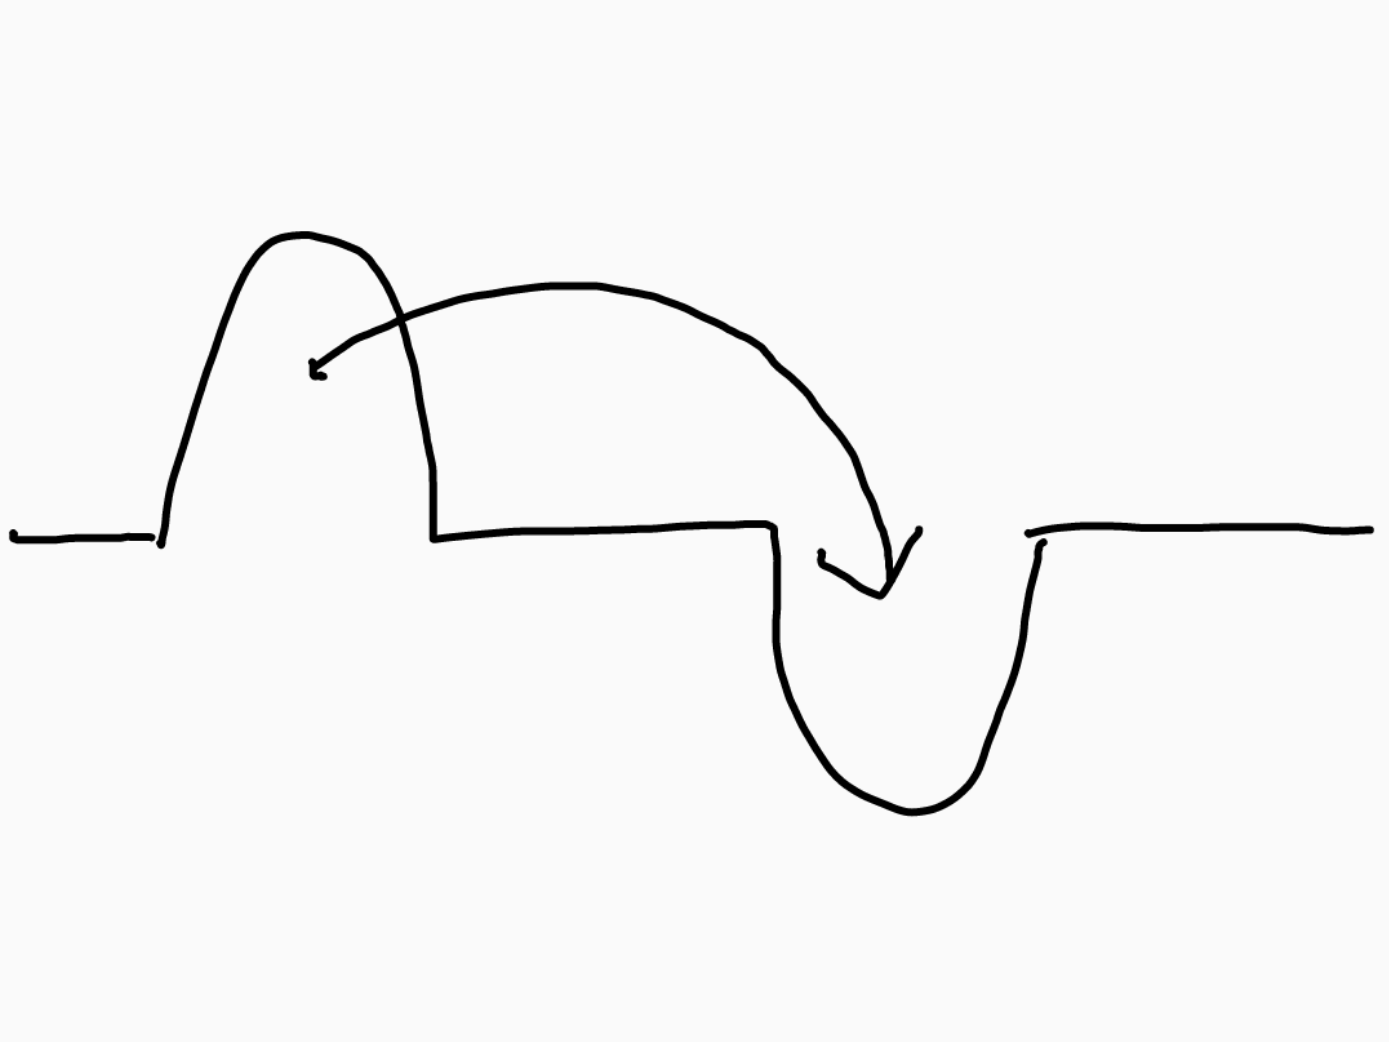
\includegraphics[scale=0.15]{1}
\end{center}
\end{figure}

Let $\mu, \nu$ be measures on $X, Y$ and $C : X\times Y \rightarrow [0, \infty]$ be the cost function.
\s

\definum{2.1} We say that $T: X\rightarrow Y$ \textbf{transports} $\mu \in \mathscr{P}(X)$ to $\nu \in \PP(Y)$(and we call $T$ a \textbf{transport map}) if
\begin{align*}
\nu(B) = \mu(T^{-1}(B)) \quad \forall \nu-\text{measurable } B \call{2.1}
\end{align*}
If $T$ is injective, then this is equivalent to saying that $\nu(T(A)) = \mu(A)$ for all $\mu$-measurable sets $A$.
\s

\begin{figure}[h]
\begin{center}
    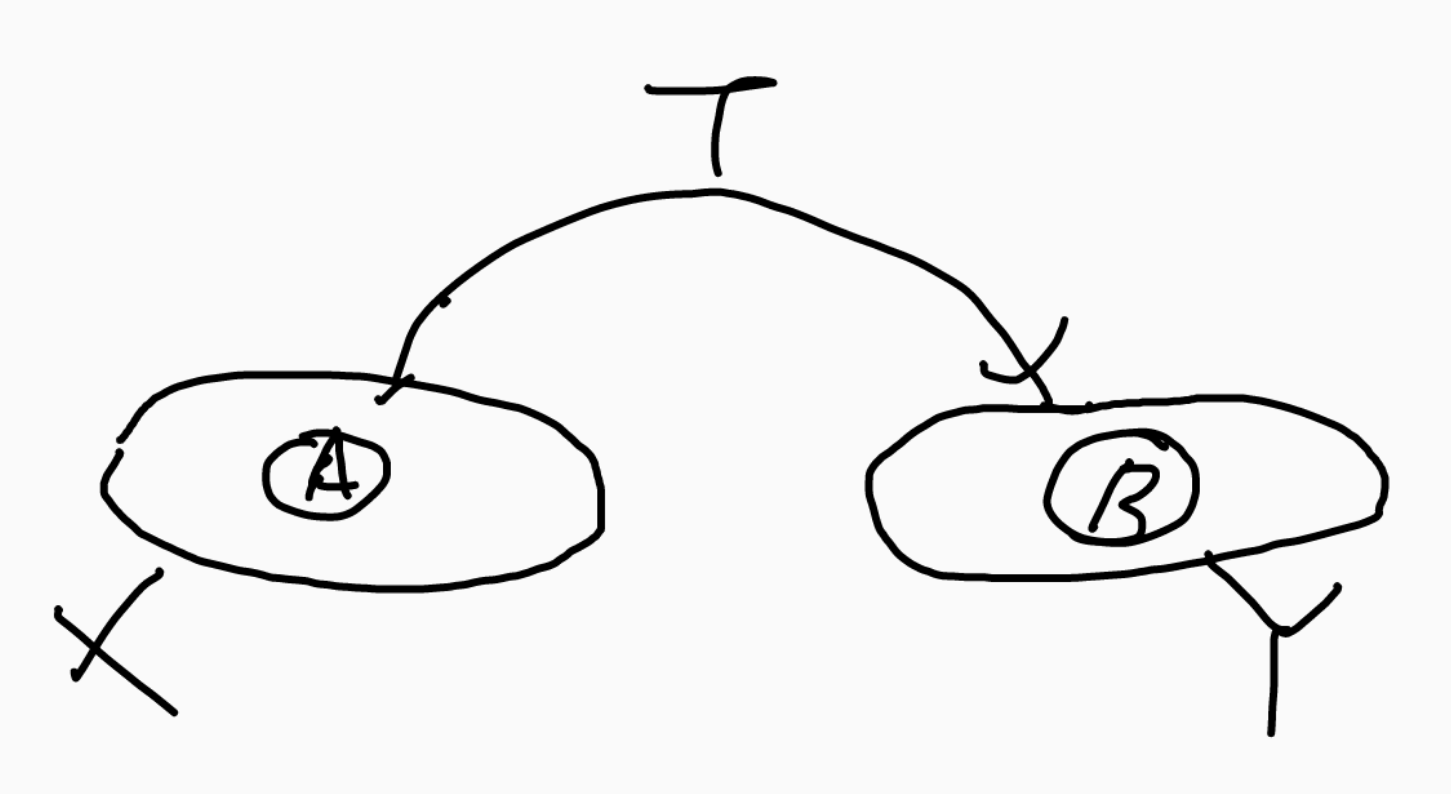
\includegraphics[scale=0.15]{2}
\end{center}
\end{figure}

Let $\mu \in \PP(X)$, $T:X\rightarrow Y$.
\s

\definum{2.2} $\mu \in \PP(X)$, $T: X\rightarrow Y$ be measurable. Then $T_{\#} \mu$ as defined in (2.1) is called the \textbf{pushforward} of $\mu$ by $T$.
\s

\subsubsection*{Existence of Transport Map}
Let $\mu, \nu$ be probability measures as above. Then can we find $T : X\rightarrow Y$ such that $T_{\#} \mu =\nu$?
\s

\textbf{Examples :}
\begin{i}
\item If $\mu = \delta_{x_1}$, $\nu = \frac{1}{2}(\delta_{y_1} + \delta_{y_2})$, we have $\frac{1}{2} = \mu(T^{-1}(y_1)) \in \{0,1\}$, so we do not have such transport map.
\item If in the discrete case with $|X|= |\{x_1, \cdots, x_n\}| = |Y| = |\{y_1, \cdots, y_n\}$, and $\mu = \frac{1}{n}\sum_{i} \delta_{x_i}$, $\nu = \frac{1}{n}\sum_i \delta_{y_i}$, then we always have the transport.(to be seen)
\item If $\mu$ and $\nu$ are absolutely continuous w.r.t. the Lebesgue measures on $X, Y$, then the transport exists.(to be seen)
\end{i} 

\subsubsection*{The Monge's Problem}

\definum{2.4} \emph{(Monge's Optimal Transport Problem)} Let $\mu \in \PP (X)$, $\nu \in \PP(Y)$ be given, then \textbf{Monge's optimal transport problem} asks to find
\begin{align*}
\text{minimize}_T \,\,\mathbb{M}(T) = \int_X C(y, T(x)) d\mu(x) \quad \text{subject to } \nu = T_{\#} \mu
\end{align*}
\s

If we assume that both measures are absolutely continuos w.r.t. the Lebesgue measure with $d\mu(x) = f(x)dx$, $d\nu(y) = g(y)dy$ and $T$ is bijective with $T, T^{-1}$ both differentiable, then (2.1) is equivalent to having $f(x) = g(T(y)) |\text{det}(\nabla T(x))|$. This is highly non-linear. So even in the simplest setting, it is often difficult to solve the Monge's problem.

\subsection{The Kantorovich Formulation}

Consider $\pi \in \PP(X\times Y)$. We want $d\pi(x,y)$ to be the amount of mass transferred from $x$ to $y$. We would have contraints $\pi(A, Y) = \mu(A)$ and $\pi(X, B) = \nu(B)$ for all measurable sets $A\subset X$, $B\subset Y$, \textit{i.e.} the amount of mass tranferred to and from a specific point is fixed. Denote the set of such $\pi$ by $\Pi(\mu,\nu)$

Note, $\Pi(\mu, \nu)$ can never be empty, as the product measures $\mu \otimes \nu$ is in $\Pi(\mu, \nu)$.
\s

\defi \emph{(Kantorovich Optimal Transport Problem)} Given $\mu \in \PP(X)$ and $\nu \in \PP(Y)$, the \textbf{Kantorovich optimal transport problem} asks to find 
\begin{align*}
\text{minimize}_{\pi \in \Pi(\mu, \nu)} \,\, \mathbb{K}(\pi) = \int_{X\times Y} C(x,y) d\pi(x,y)
\end{align*}
\s

Obviously, the Monge's problem and the Kantorovich's problems are not equivalent - the existence of trasport map $T$ is not guaranteed for the Monge's problem in the first place. However, we can establish an inequality relation betwenn $\inf \mathbb{K}{\pi}$ and $\inf \mathbb{M}(T)$.

\quad Let us assume that $\exists T^{\dagger} : X\rightarrow Y$ is optimal in the Monge's problem, and let $d\pi(x,y) = d\mu(x) \delta_{y = T^{\dagger} x}$. Then
\begin{align*}
& \pi(A \times Y) = \int_A \delta_{T^{\dagger}(x) \in Y} d\mu(x) = \mu(A) \\
& \pi(X\times B) = \int_X \delta_{T^{\dagger}(x)\in B} d\mu(x) = \mu((T^{\dagger})^{-1}(B)) = T_{\#}^{\dagger} \mu(B) = \nu(B)
\end{align*}
and
\begin{align*}
\int_{X\times Y}C(x,y) d\pi(x,y) = \int_X \int_Y C(x,y) \delta_{y = T^{\dagger}x} dy d\mu(x) = \int_X C(x,T^{-1}x) d\mu(x)  
\end{align*}
so we have $\inf \mathbb{K}(\pi) \leq \inf \mathbb{M}(T)$.
\s

\newday

(25th January, Friday)
\s

Last time, we have seen two formulations of optimal transport problem :
\begin{align*}
\min_{T : T_{\#}\mu =\nu} \int_X c(x, T(x))d\mu(x) &\quad \text{(Monge)}\,\, ; \\
\min_{\pi \in \Pi(\mu, \nu)} \int_{X\times Y} c(x,y) d\pi(x,y) &\quad \text{(Kantorovich)}
\end{align*}
If we find an optimal plan $\pi^{\dagger} : d\pi^{\dagger}(x,y) = d\mu(x) \delta_{y= T(x)}$, then $T$ is optimal transport map and $\inf \mathbb{M}(T) \leq \inf \mathbb{K}(\pi)$. So combined with the inequality seen earlier, under a sufficient setting, the inequality is in fact an equality.
\s

\subsubsection*{Interpolations}

Monge : $\mu_t := \Big( (1-t)id + tT^{\dagger} \Big)_{\#} \mu$. (compare with $\mu_t = (1-t)\mu + tv$)

Kantorovich : let $\mu =\sum_{i=1}^m \alpha_i \delta_{x_i}$, $\nu =\sum_{j=1}^n \beta_i \delta_{u_j}$, $c_{ij} = c(x_i, y_j)$ then the problem is written as
\begin{align*}
& \min_{\pi} \sum_{i=1}^m \sum_{j=1}^n c_{ij} \pi_{ij} \\
& \text{subject to} \quad \pi_{ij} \geq 0, \,\,\sum_{i=1}^m \pi_{ij} =\beta_j,\,\, \sum_{j=1}^n \pi_{ij} = \alpha_i
\end{align*}
This linear program. The advantae for this setting is that it can also be written as
\begin{align*}
\inf_{\pi \geq 0, c^T \pi = (\mu^T, \nu^T)^T} c\cdot\pi = \sup_{C(\varphi^T, \phi^T)\leq c}(\mu \cdot \varphi + \nu \cdot \phi)
\end{align*}
\emph{[Write in more detail later]}

\subsection{Existence of Transport Plans}

\propnum{2.6}  Let $\mu \in \mathscr{P}(X)$, $\nu \in \mathscr{P}(Y)$, $X, Y$ Polish spaces and $c: X\times Y \rightarrow [0, \infty]$ is lower semi-continuous. Then $\exists \pi^{\dagger} \in \Pi(\mu, \nu)$ such that
\begin{align*}
\mathbb{K}(\pi^{\dagger}) = \min_{\pi \in \Pi(\mu, \nu)}\mathbb{K}(\pi)
\end{align*}
\begin{p}
\pf $\Pi(\mu, \nu)$ is non-empty. Let $\delta >0$ and pick $K\subset X$, $L\subset Y$ compact so that
\begin{align*}
\mu(X\backslash K) \leq \delta, \quad \nu(Y \backslash L) \leq \delta
\end{align*}
Take $(x, y) \in (X,Y) \backslash(K \times L)$. Then either $x\not\in K$ or $y\not\in L$, hence $(x,y) \in X\times (Y\backslash L)$ or $(x,y) \in (X\backslash K) \times Y$. Therefore, $\forall \pi \in \Pi(\mu, \nu)$, we have
\begin{align*}
\pi((X\times Y)\backslash (K\times L)) \leq \pi(X\times (Y\backslash L)) + \pi((X\backslash K) \times Y) \\
= \nu(Y\backslash L) + \mu(X\backslash K) \leq 2\delta
\end{align*}
so we see that $\Pi(\mu, \nu)$ is tight.

\quad We want to see that $\Pi(\mu, \nu)$ is weak-* closed. So consider any weakly-* converging seqeunce $\pi_u \in \Pi(\mu, \nu) \xrightarrow{w-*} \pi \in M(X\times Y)$, \textit{i.e.} $\forall f\in C_b^0(X\times Y)$, $\int_{X\times Y} f(x,y) d\pi_u(x,y) \rightarrow \int_{X\times Y} f(x,y) d\pi(x,y)$. Let $f(x,y) = \tilde{f}(x)$ be continuous and bounded. Then
\begin{align*}
\int_{X\times Y} f(x,y) d\pi_u(x,y) = \int_{X} \tilde{f} (x) d\mu(x) \rightarrow \int_X f (x) d\pi(x,y) = \int_{X} \tilde{f}(x) dP_{\#}^X \pi(x)
\end{align*}
where $P^X(x,y) = x$ is the projection. Hence for all $\tilde{f} \in C_b^0 (X)$, $\int_X \tilde{f}(x)d\mu(x) = \int_X \tilde{f}(x) dP_{\#}^X \pi(y)$ so $P_{\#}^X = \mu$. Similarly, $P_{\#}^Y \pi =\nu$ so we see that $\pi \in \Pi(\mu, \nu)$. Therefore, $\Pi$ is weakly-* closed subset of $\mathscr{M}(X,Y)$.

\quad Let $\pi_n \in \Pi(\mu, \nu)$ be a minimising sequence, \textit{i.e.} $\mathbb{K}(\pi_n) \rightarrow \inf_{\pi \in \Pi}\mathbb{K}(\pi)$. Then by \emph{Prohorov's theorem} and weak-* closedness of $\Pi(\mu, \nu)$, we may find $\pi^{\dagger} \in \Pi(\mu, \nu)$ and a subsequence $\pi_{n_j}$ with $\pi_{n_j} \rightarrow \pi^{\dagger}$. Since $c$ is bounded from below and continuous, we have
\begin{align*}
\int_{X\times Y} c(x,y)d\pi^{\dagger}(x,y) \leq \liminf_{j\rightarrow \infty} \int_{X,Y} c(x,y) d\pi_{n_j}(x,y) = \inf_{\pi \in \Pi(\mu, \nu)}\mathbb{K}(\pi)
\end{align*}
\eop
\end{p}


\section{Special cases}
We  now just consider the special cases in which :
\begin{i}
\item[1.] $\mu, \nu$ on the real line \emph{or},
\item[2.] $\mu, \nu$ on the discrete space
\end{i}

We will generalise the conditions on $\mu$ and $\nu$ later on based on the observations obtained in this chapter.

\subsection{Optimal Transport in 1D}

Let $\mu, \nu\in \mathscr{P}(\reals)$ with culmulative distribution functions(CDF) $F$ and $G$ respectively.  Then $F,G$ are right-continuous, non-decreasing, $F(-\infty) =0$ and $F(+\infty) =1$. Define
\begin{align*}
&F^{-1}(t) : = \inf \{x\in \reals : F(x)>t \}\\
\Rightarrow \quad & F^{-1}(F(x)) \geq x, \quad F(F^{-1}(t))\geq t
\end{align*}
If $F$ is invertible, these inequalities are in fact equalities.
\s

\thmnum{3.1} Let $\mu, \nu \in \mathscr{P}(\reals)$ with culmulative distribution functions $F$ and $G$ resp. Let $c(x,y)= d(x-y)$, for a function $d$ convex and continuous. Let $\pi^{\dagger} \in \mathscr{P}(\reals^2)$ with culmulative distribution function $H(x,y) = \min\{F(x), G(y)\}$. Then $\pi^{\dagger} \in \Pi(\mu, \nu)$, $\pi^{\dagger}$ optimal for the Kantorovich problem with cost function $c(x,y)$. Moreover,
\begin{align*}
\min_{\pi \in \Pi(\mu, \nu)}\mathbb{K}(\pi ) =\int_0^1 d(F^{-1}(t) - G^{-1}(t))dt
\end{align*}
\s

\corrnum{3.2} Let $\mu$ and $\nu$ be as in the theorem.
\begin{i}
\item[(1)] If $c(x,y) = |x-y|$, the optimal transport distance, we have
\begin{align*}
\inf_{\pi \in \Pi(\mu, \nu)} \mathbb{K}(\pi) = \int_{\reals} |F(x) - G(x)| dx
\end{align*}
\item[2)] If $\mu$ does not give mass to atoms, then 
\begin{align*}
\min_{\pi \in \Pi(\mu, \nu)} \mathbb{K}(\pi) = \min_{T: T_{\#}\mu =\nu} \mathbb{M}(T)
\end{align*}
and $T^{\dagger} = G^{-1}\circ F$ is a minimiser to Monge's optimal transport prolem, \textit{i.e.} $T_{\#}^{\dagger} \mu = \nu$ and $\inf_{T: T_{\#} \mu = \nu} \mathbb{M}(T) = \mathbb{M}(T^{\dagger})$.
\end{i}
\s

\newday

(28th January, Monday)
\s

(Example Classes : 7th Feburary, 21st Feburay, 7th March and one next term, Thursdays)
\s

\textbf{Recap :}
\begin{subproof}
\definum{2.2} \emph{(Monge Optimal Transport Problem (MOT))} Given $\mu \in \PP(X), \nu\in \PP(Y)$, minimize $\mathbb{M}(T) =\int_X c(x, T(x)) d\mu(x)$ over all measurable $T:X\rightarrow Y$ such that $T_{\#} \mu = \nu$.

\definum{2.3} \emph{(Kantorovich Optimal Transport Problem (KOT))} Given $\mu\in \PP(X),\nu\in\PP(Y)$, minimize $\mathbb{K}(\pi) = \int_{X\times Y} c(x,y) d\pi(x,y)$ over all $\pi \in \Pi(\pi, \nu)$.
\s

If $T^{\dagger}$ minimizes MOT problem, then define $\pi^{\dagger} = (id \times T^{\dagger})_{\#} \mu \in \Pi(\mu, \nu)$, and so
\begin{align*}
\min_{\pi \in \Pi(\mu, \nu)} \mathbb{K}(\pi) \leq \mathbb{K}(\pi^{\dagger}) = \mathbb{M}(T^{\dagger})
\end{align*}
and so $\min_{\pi} \mathbb{K}(\pi) \leq \inf_T \mathbb{M}(T)$.

\quad This argument also works without assuming the existence of minimiser $T^{\dagger}$ by taking a sequence of $T$'s such that $\mathbb{M}(T)$ converges to the minimum.
\s

\propnum{2.4} Let $\mu \in \PP(X),\nu\in\PP(Y)$, $X,Y$ Polish spaces, $c:X\times Y \rightarrow [0, \infty)$ lower semicontinuous(lsc), then $\exists \pi^{\dagger} \in \Pi(\mu, \nu)$ that minimises KOT.
\begin{p}
\pf Uses direct method from the calculus of variation. That is, the ``compactness of lsc $\Rightarrow$ $\exists$ minimiser".
\end{p}
\end{subproof}
\s

Let $\mu, \nu \in \PP(\reals)$, with culmulative distribution function $F,G$ respectively. We also defined the \textbf{generalized inverse} of a cdf $F$ on $[0,1]$ by
\begin{align*}
F^{-1}(t) = \inf \{x\in \reals : F(x) > t\}
\end{align*}
then $F^{-1}(F(x))\geq x$ and $F(F^{-1}(t)) \geq t$.
\s

\thmnum{3.1} Let $\mu, \nu \in\PP(\reals)$ with cdf $F,G$ respectively. Assume $c(x,y) =d(x,y)$ for some $d$ convex (and continuous).  Let $\pi^{\dagger}$ be the measure on $\reals^2$ with cdf $H(x,y) = \min\{F(x), G(y)\}$. Then $\pi^{\dagger} \in \Pi(\pi, \nu)$ is a minimiser of KOT problem at the OT cost is
\begin{align*}
\min_{\pi \in \Pi(\mu, \nu)} \mathbb{K}(\pi) = \int_0^1 d(F^{-1}(t), G^{-1}(t))dt
\end{align*}
\begin{p}
\textbf{Idea :} $H(x,y)$ has the following interpretation - we can not bring out from space $X$ at $x$ more than we have got ($F(x)$) and can not put in space $Y$ at $y$ than we need ($G(y)$).

\quad We will come back to the actual proof later.
\end{p}
\s

\corrnum{3.2} Under these assumptions of \textbf{Theorem 3.1}, the following hold :
\begin{i}
\item[1.] If $c(x,y) = |x-y|$, then the KOT cost is the $L^1$ distance between cdf's, \textit{i.e.}
\begin{align*}
\min_{\pi \in \Pi(\mu,\nu)}\mathbb{K}(\pi) = \int_{\reals} |F(x) - G(x)| dx
\end{align*}
\item[2.] If $\mu$ does not give mass to small sets (sets of Hausdorff dimension < 1, or has no atoms, or its culmulative distribution function is continuous) then
\begin{align*}
\min_{\pi \in \Pi(\mu, \nu)} \mathbb{F}(\pi) = \min_{T: T_{\#}\mu =\nu} \mathbb{M}(T)
\end{align*}
and furthermore $T^{\dagger} = G^{-1} \circ F$ is a minimiser to the MOT problem.
\end{i}
\begin{p}
\pf \begin{i}
\item[1.] By \textbf{Theorem 3.1}, it is enough to show that
\begin{align*}
\int_0^1 |F^{-1}(t) - G^{-1}(t)| dt = \int_{\reals} |F(x) - G(x)|dx
\end{align*}
Define 
\begin{align*}
A\subset \reals^2 \text{ by }A= \{(x,y) : \min \{F(x), G((x) \} \leq t \leq \max \{F(x), G(x) \}, x\in \reals
\end{align*}

\begin{figure}[h]
\begin{center}
    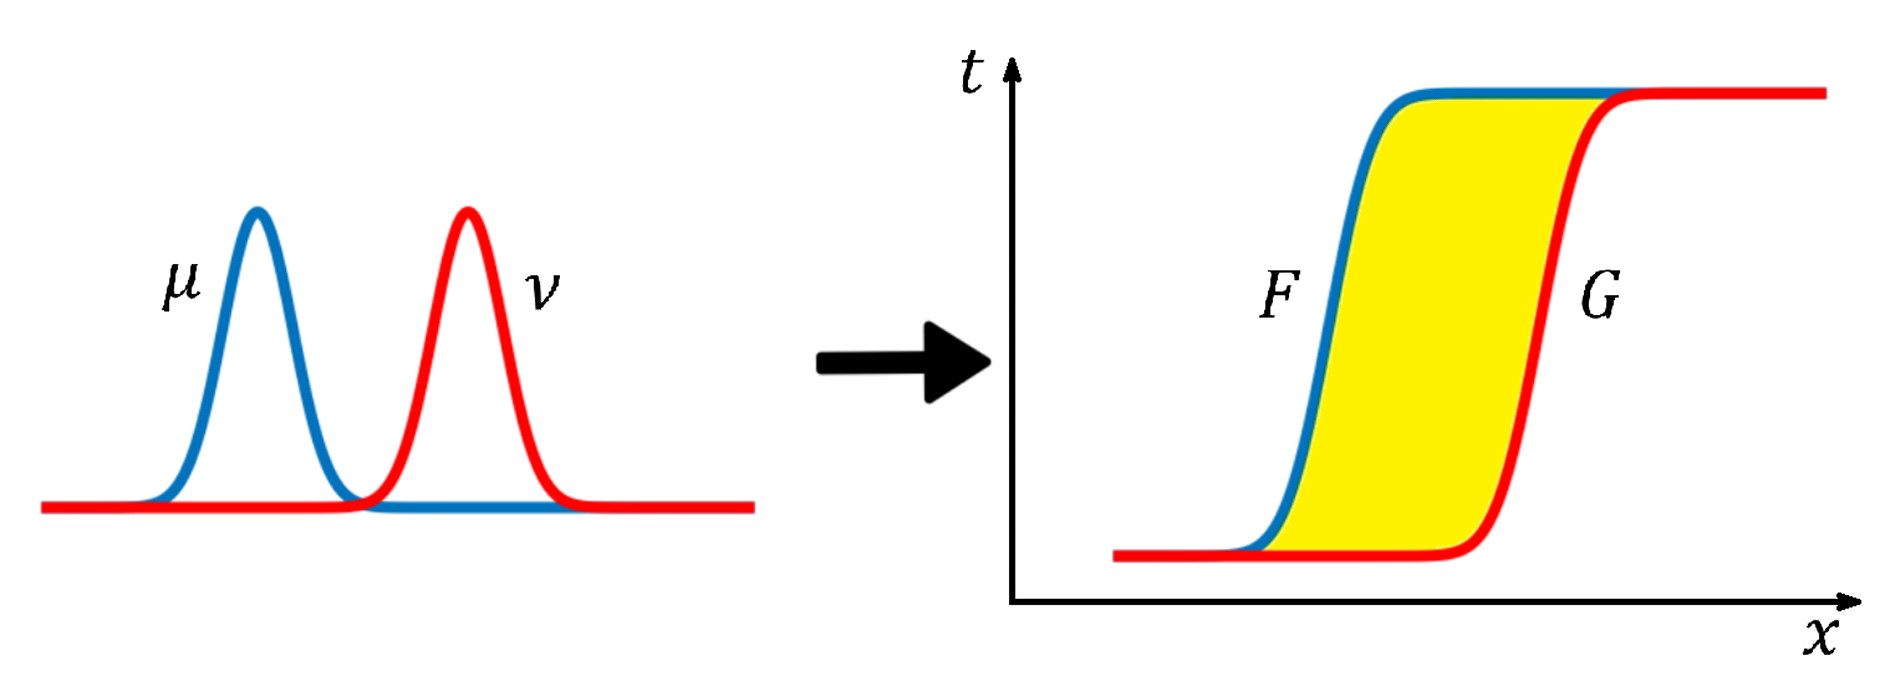
\includegraphics[scale=0.15]{3}
\end{center}
\end{figure}

Note $A = \{(x,y) : \min \{F^{-1}(t), G^{-1}(t)\}\leq x\leq \max \{F^{-1}(t), G^{-1}(t)\}, t\in [0,1] \}$ upto a set of Lebesgue measure 0. By Fubini's theorem,
\begin{align*}
\int_{\reals}\int_{\min \{F(x), G(x)\}}^{\max \{F(x), G(x)\}} 1 dtdx = \int_0^1 \int_{\min \{F^{-1}(t), G^{-1}(t)\}}^{\max \{F^{-1}(t), G^{-1}(t)\}} 1dxdt
\end{align*}
so
\begin{align*}
&\int_{\reals} \max \{F(x), G(x)\} - \min \{F(x), G(x)\} dx \\
=&\int_0^1 \max \{F^{-1}(t), G^{-1}(t)\} - \min \{F^{-1}(t), G^{-1}(t)\} dt \\
\Rightarrow \quad &\int_{\reals} |F(x)- G(x)| dx =\int_0^1 |F^{-1}(t) - G^{-1}(t)|dt
\end{align*}
using $|a-b| = \max (a,b) - \min(a,b)$.
\end{i}
\item[2.] By composition of maps (\textbf{Proposition 2.3}) we have $T_{\#}^{\dagger} = G_{\#}^{-1}(F_{\#}\mu)$. We cliam (i) $G_{\#} \mathscr{L} =\nu$ and (ii) $F_{\#} \mu = \mathscr{L}$ where $\mathscr{L}$ is the Lebesgure measure on $[0,1]$. Assumiing (i) and (ii), we have $T_{\#}^{\dagger} \mu = G_{\#}^{-1} \mathscr{L} =\nu$.

\quad To prove (i),
\begin{align*}
G_{\#}^{-1} \mathscr{L} ((-\infty, y]) &= \mathscr{L} (\{t: G^{-1}(t) \leq y\}) = \mathscr{L} (\{t : G(y)\geq t\}) \\
&= G(y) = \nu ((-\infty, y])
\end{align*}
and therefore $G^{-1}_{\#} \mathscr{L}=\nu$.

\quad For (ii), since $F$ is continuous (as $\mu$ does not give mass to atoms) so $\forall t\in (0,1)$, $F^{-1}([0,t])$ is closed. Hence $\forall t\in (0,1)$, $\exists x_t$ such that
\begin{align*}
F^{-1}([0,t]) =(-\infty, x_t] \quad \text{and }\quad F(x_t) =t
\end{align*}
So $F_{\#}([0,t]) = \mu(x: F(x)\leq t) = \mu(x: x\leq x_t) = F(x_t) =t$. Hence $F_{\#}\mu = \mathscr{L}$.

\quad Now by \textbf{Theorem 3.1},
\begin{align*}
\inf \mathbb{K}(\pi) &= \int_0^1 d(F^{-1}(t)- G^{-1}(t)) dt\\
&= \int_0^1 d(F^{-1}(t) - G^{-1}(t)) d(F_{\#} \mu(t)) \\
&\geq \int_{\reals} d(x- G^{-1}(F(x))) d\mu(x) \quad \text{(by \textbf{Proposition 1.5})} \\
&= \int_{\reals} d(x- T^{\dagger}(x))d\mu(x) \\
&= \mathbb{M}(T^{\dagger}) \geq \inf_{T: T_{\#} =0} \mathbb{M}(T) \geq \inf \mathbb{K}(\pi)
\end{align*}
where the last inequality follows from general relation between $\inf \mathbb{M}$ and $\inf \mathbb{K}$. This implies all inequalities are equalities, so $\min \mathbb{K}(\pi) = \min \mathbb{M}(T) = \mathbb{M}(T^{\dagger})$.

\eop
\end{p}
\s

\newday

(30th January, Wednesday)
\s

Example classes : MR11, 4pm - 5.5pm, (1) 7th Feb, (2) 21st Feb, (3) 7th March, one next term.
\s

\textbf{Recap :} for $\mu, \nu \in \PP(\reals)$, $F(x) = \int_{-\infty}^x d\mu(x)$, $G(y) = \int_{-\infty}^y d\nu(y)$.
\s

We chage our notation, $F^{-1}(t) = \inf \{x\in \reals : F(x)\geq t \}$... so we would have $F(F^{-1}(t)) \leq t$.
\s

\thmnum{3.1} $\mu, \nu \in \PP(\reals)$ with culmulative distribution function $F, G$ respectively. Assume $c(x,y) = d(x-y)$ where $d$ is convex and continuous. Let $\pi^{\dagger}$ be the measure on $\reals^2$ with culmulative distribution function $H(x,y) = \min \{F(x), G(y)\}$. then $\pi^{\dagger} \in \Pi(\mu, \nu)$ and is a minimiser of KOT problem and the optimal cost is
\begin{align*}
\min_{\pi \in \Pi(\mu, \nu)} \mathbb{K}(\pi) = \int_0^1 d(F^{-1}(t) - G^{-1}(t))dt
\end{align*}

\s

The key idea in the proof of \textbf{Theorem 3.1} is monotonicity :
\s

\defi We say \textbf{$\Gamma \subset \reals^2$ is monotone with respect to $d$} if $\forall (x_1, y_1), (x_2, y_2) \in \Gamma$, we have $d(x_1 -y_1) + d(x_2 -y_2) \leq d(x_1-y_2) +d(x_2-y_1)$.

\quad This definition is given for 1D, but it can be generalised to higher dimensions. It is also used in convex analysis, \textit{e.g.} the subdifferential of a convex function satisfies monotonicity property.
\s

\textbf{Intuition :} the support of an optimal transport plan should be monotone. If $\text{supp}(\pi)= \Gamma$, then $(x_1,y_1) , (x_2, y_2) \in \Gamma$ implies that mass is transported from $x_i$ to $y_i$ ($i=1,2$). If $d(x_1-y_1) +d(x_2-y_2) \geq d(x_1-y_2) + d(x_2-y_2)$, \textit{i.e.} cheaper to transport mass from $x_1$ to $y_2$ and $x_2$ to $y_1$, then to tranport from $x_i$ to $y_i$ ($i=1,2$).
\s

\textbf{Example :} Let $\Gamma = \{(x,y) : f(x)=y\}$ with $f,d$ increasing. Then $\Gamma$ is monotone. \emph{(Exercise)}.
\s

\propnum{3.3} Let $\mu, \nu \in\PP(\reals)$. Assume $\pi^{\dagger} \in \Pi(\mu, \nu)$ is an optimal plan for the cost function $c(x,y) = d(x,y)$ where $d$ is continuous. Then for all $(x_1, y_1), (x_2, y_2) \in \text{supp}(\pi)$, we have
\begin{align*}
d(x_1 -y_1) + d(x_2-y_2) \leq d(x_1-y_2)+d(x_2-y_1)
\end{align*}
\textit{i.e.} $\text{supp}(\pi)$ is \emph{cyclically monotone}.
\begin{p}
\pf Assume that $\exists \eta>0$ such that
\begin{align*}
d(x_1-y_1) +d(x_2-y_2) - d(x_1-y_2) -d(x_2-y_1) > \eta
\end{align*}
Let $I_1, I_2, J_1, J_2$ be closed intervals with the following properties :
\begin{align*}
\begin{cases}
1. \,\, x_i \in I_i, y_i \in J_i, \quad i=1,2 \\
2. \,\, |d(x-y) - d(x_i -y_j)| \leq \epsilon \quad \text{for }x\in I_i, y\in J_i, \,\, i,j=1,2, \text{ when } \epsilon < \eta/4\\
3. \,\, I_i \times J_j \text{ are disjoint} \\
4. \,\, \pi^{\dagger}(I_1\times J_1) = \pi^{\dagger}(I_2\times J_2) =\delta >0
\end{cases}
\end{align*}
\begin{figure}[h]
\begin{center}
    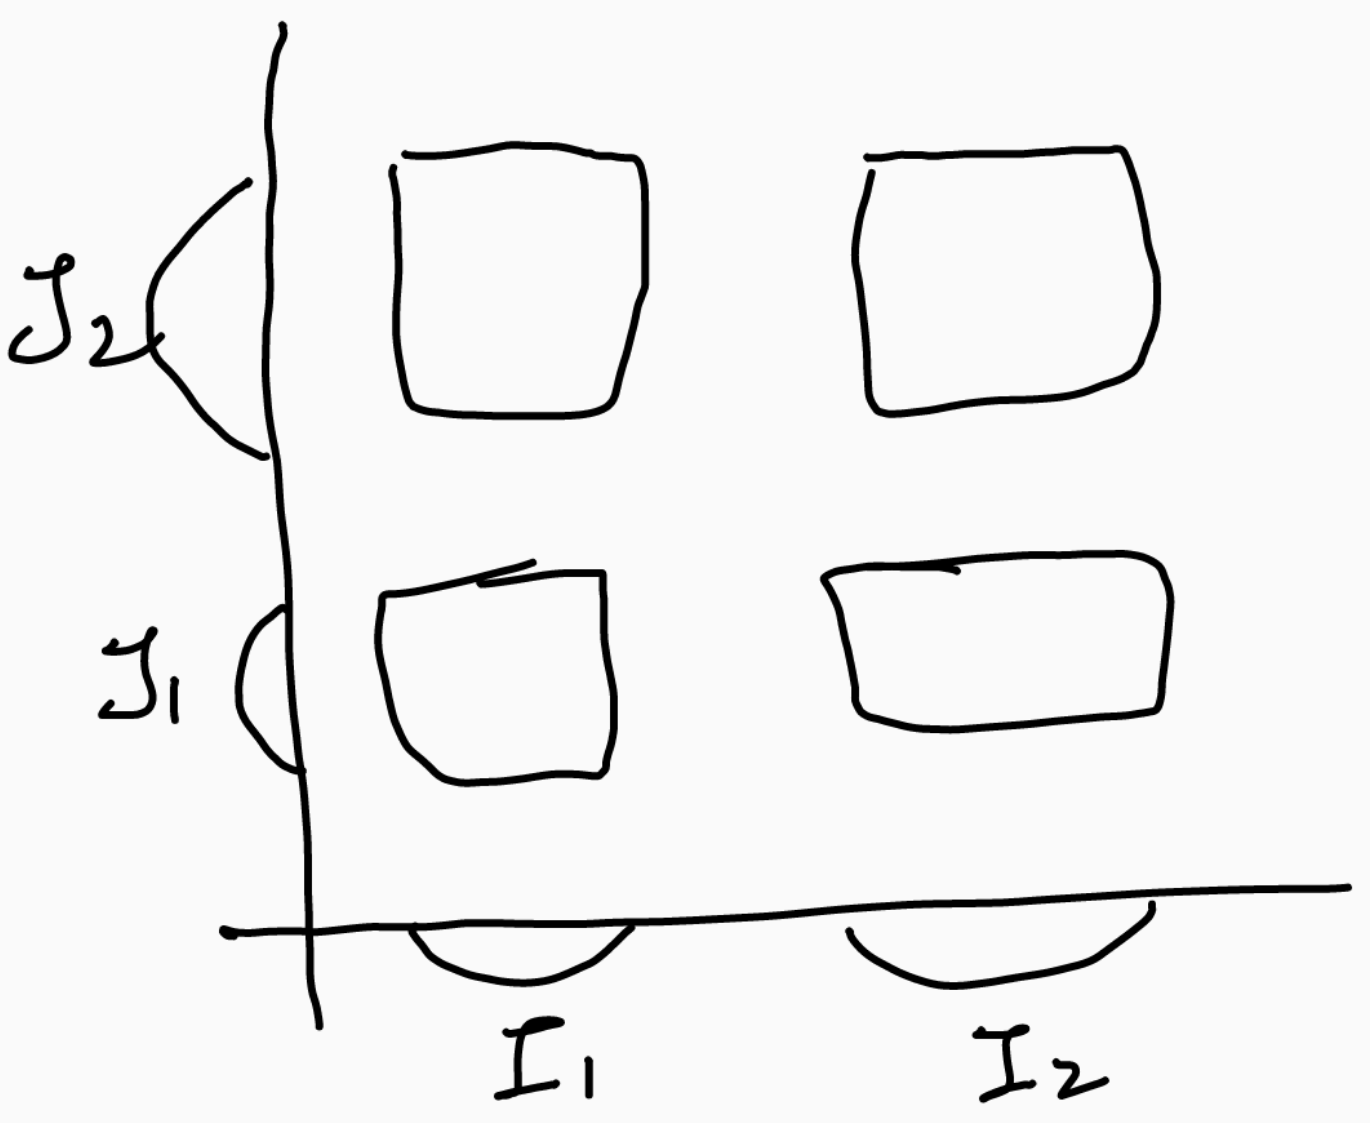
\includegraphics[scale=0.15]{4}
\end{center}
\end{figure}
Properties 1-3 can be satisfied by chossing the intervals $I_i, J_j$ small enough. Property 4 may not hold, but we at the moment assume it for simplicity. At the end of the proof, we will discuss how to avoid (4).
\s

\textbf{Idea :} current plan ($\pi^{\dagger}$) is $I_1 \mapsto J_1$, $I_2 \mapsto J_2$. We argue that $I_1 \mapsto J_2$, $I_2 \mapsto J_1$ provides a transport plan with lower cost.
\s

Let $\tilde{\mu}_i = P_{\#}^X \pi^{\dagger}|_{I_i\times J_i}$, $\tilde{\nu}_i = P_{\#}^Y \pi^{\dagger}|_{I_i\times J_i}$, $i=1,2$, where $P^X$ is the projection to $X$ and $P^Y$ is the projection to $Y$. Choose any couplings $\tilde{\pi}_{12} \in \Pi(\tilde{\mu}_1, \tilde{\nu}_2)$, $\tilde{\pi}_{21} \in \Pi(\tilde{\mu_2}, \tilde{\nu}_1)$.

\quad Define $\tilde{\pi}$ to satisfy
\begin{align*}
\tilde{\pi}(A\times B) = \begin{cases}
\pi^{\dagger}(A\times B) \quad &\text{if } (A\times B) \cap (I_i \times J_j) =\phi, \forall i,j \\
0 \quad &\text{if } A\times B \subset I_i \times J_i,\,\, i=1,2 \\
\pi^{\dagger} (A\times B) + \tilde{\pi}_{12}(A\times B) \quad &\text{if } A\times B \subset I_1\times J_2\\
\pi^{\dagger}(A\times B) + \tilde{\pi}_{21}(A\times B) \quad &\text{if } A\times B \subset I_2\times J_1 
\end{cases}
\end{align*}
\end{p}
\s

\newday

(1st February, Friday)
\s

\begin{p}
\textbf{proof continued)} We check that $\tilde{\pi}$ defined above is in $\Pi(\mu, \nu)$
\begin{i}
\item[(i)] for $B\subset \reals$ with $B\cap (J_1 \cup J_2) = \phi$, we have $\tilde{\pi}(\reals \times B) = \pi^{\dagger}(\reals \times B) = \nu(B)$.
\item[(ii)] for $B\subset \reals$ with $B\subset J_1$, 
\begin{align*}
\tilde{\pi}(\reals \times B) &= \tilde{\pi}((\reals \backslash (I_1 \cup I_2))\times B) + \tilde{\pi}(I_1\times B) + \tilde{\pi}(I_2 \times B)  \\
&= \pi^{\dagger}((\reals \backslash (I_1 \cup I_2))\times B) + 0 + \pi^{\dagger}(I_2 \times B) + \tilde{\pi}_{21}(I_2\times B) \\
&= \pi^{\dagger}((\reals \backslash I_1)\times B) + \pi^{\dagger}(I_1 \times B) \\
&=\pi^{\dagger}(\reals \times B)  =\nu(B)
\end{align*}
where the third equality follows because $\tilde{\pi_{21}}(I_2\times B) = \tilde{\nu}_1 (B) = \pi^{\dagger}(I_1 \times B)$.

\item[(iii)] Similar computations when $B\subset J_2$ shows $\tilde{\pi}(\reals \times B) = \nu(B)$ for all $B\subset \reals$ measurable.

And analogously, $A\subset \reals$, $\tilde{\pi}(A\times \reals) = \mu(A)$. Hence $\tilde{\pi} \in \Pi(\mu, \nu)$.
\end{i}
Now since $\pi^{\dagger}$ and $\tilde{\pi}$ only differ on $(I_1 \cup I_2) \times (J_1 \cup J_2)$, we have
\begin{align*}
\mathbb{K}(\pi^{\dagger}) - \mathbb{K}(\tilde{\pi}) =& \int_{\reals \times \reals} d(x-y) d\pi^{\dagger}(x,y) - \int_{\reals \times \reals} d(x-y) d\tilde{\pi}(x,y) \\
=& \int_{(I_1 \times J_1)\cup (I_2 \times J_2)} d(x-y) d\pi^{\dagger}(x,y)  \\
&- \int_{I_1 \times J_2} d(x-y) d\tilde{\pi}(x,y) - \int_{I_2 \times J_1} d(x-y) d\tilde{\pi}(x,y) \\
\geq & \delta (d(x_1-y_1) - \epsilon) + \delta((d(x_2-y_2)  - \epsilon) - \delta(d(x_1-y_2)+\epsilon) - \delta(d(x_2-y_1) + \epsilon) \\
= &  \delta \big( d(x_1-y_1) + d(x_2-y_2) - d(x_1-y_2)-d(x_2-y_1) -4\epsilon\big) \\
\geq & \delta \big(\eta - 4\epsilon \big) > 0
\end{align*}
which contradicts with the fact that $\pi^{\dagger}$ is optimal. Hence, no such $\eta>0$ exists.
\s

Finally, as promised, let us discuss how we can modify the proof if Property 4 does not hold :
\begin{subproof}
: Wlog, assume $\pi^{\dagger}(I_1\times J_1) > \pi^{\dagger}(I_2\times J_2)$. We let 
\begin{align*}
\tilde{\mu}_1 = \frac{\pi^{\dagger}(I_2 \times J_2)}{\pi^{\dagger}(I_1 \times J_1)} P_{\#}^{X} \pi^{\dagger} |_{I_1 \times J_1} \\
\tilde{\nu}_1 = \frac{\pi^{\dagger}(I_2 \times J_2)}{\pi^{\dagger}(I_1 \times J_1)} P_{\#}^{Y} \pi^{\dagger} |_{I_1 \times J_1}
\end{align*}
and leave $\tilde{\mu}_2$, $\tilde{\nu}_2$ unchanged. Let $\tilde{\pi}$ be as before apart from when $A\times B \subset I_1 \times J_1$ - if $A\times B \subset I_1 \times J_1$, then we let
\begin{align*}
\tilde{\pi}(A\times B) = \pi^{\dagger}(A\times B) \Big(1- \frac{\pi^{\dagger}(I_2 \times J_2)}{\pi^{\dagger}(I_1\times J_1)} \Big)
\end{align*}
Now the notations are more heavy, but nonetheless the theorem follows from exactly the same method.
\end{subproof}
\eop
\end{p}
\s

Now we prove the main theorem of the chapter.
\s

\begin{p}
\textbf{proof of Theorem 3.1)} First, assume $d$ is stricly convex. By \textbf{Proposition 2.4}, we may find $\pi^* \in \Pi(\mu, \nu)$ that is optimal for KOT problem, \textit{i.e.}  $\min_{\pi} \mathbb{K}(\pi) = \mathbb{K}(\pi^{*})$. We show $\pi^* =\pi^{\dagger}$, where $\pi^{\dagger}$ is as in the statement of the theorem.

\quad By \textbf{Proposition 3.3.}, $\Gamma = \text{supp}(\pi^*)$ is \emph{monotone}. Let $(x_i,y_i) \in \Gamma$, $i=1,2$. We claim that if $x_1<x_2$ then $y_1\leq y_2$.
\begin{subproof}
: Assume $y_1 >y_2$. Let $a= x_1 -y_1$, $b=x_2-y_2$ and $\delta = x_2 -x_1>0$. We know fromm monotonicity
\begin{align*}
d(a) + d(b) \leq d(b-\delta) + d(a+ \delta)
\end{align*}
Let $t =\frac{\delta}{b-a} = \frac{x_2 -x_1}{(x_2-x_1)+(y_1-y_2)}$. Then $t\in (0,1)$ \emph{iff} $y_1-y_2 >0$. While
\begin{align*}
b-\delta = (1-t)b + tb -\delta =(1-t)b +t \Big(b- \frac{\delta}{t}\Big) = (1-t)b + t(b-b+a) = (1-t)b +ta
\end{align*} 
Similarly, $a+ \delta = tb + (1-t)a$. So by strict convexity,
\begin{align*}
d(b-\delta) + d(a+ \delta) <& (1-t) d(b) + td(a) + td(b) + (1-t)d(a) \\
=& d(b) + d(a)
\end{align*}
which cotradicts monotonicity. Hence $t\not \in(0,1)$ so $y_1 \leq y_2$.
\end{subproof}
To show $\pi^{\dagger} = \pi^*$, we show $\pi^*( (-\infty, x] \times (-\infty, y] ) = \min \{ F(x), G(y)\}$.
\begin{subproof}
: Let $A= (-\infty, x] \times (y, \infty)$, $B= (x, \infty) \times (-\infty, y]$. Then $\pi^*(A)$ and $\pi^*(B)$ can not both be positive - indeed, if $\Gamma =\text{supp}(\pi^*)$, $(x_1,y_1)\in A\cap \Gamma$ and $(x_2, y_2) \in B\cap \Gamma$, then $x_1 <x_2$ and $y_2 >y_1$ which can not be the case by the result right above. This implies
\begin{align*}
\pi^*((-\infty, \pi ] \times (-\infty, y]) =& \min \{ \pi^* \big(( (-\infty, x] \times (-\infty, y]) \cup A \big), \pi^* \big(((-\infty, x] \times (-\infty, y]))\cup B \big) \} \\
= &\min \{ \pi^* \big((-\infty, x] \times \reals \big), \pi^* \big(\reals \times (-\infty,y] \big)\} \\
=&\min \{\mu((-\infty, x]), \nu(-\infty, y]\} \\
=& \min \{ F(x), G(y) \}
\end{align*}
\end{subproof}
\end{p}
\s

\newday

(4th February, Monday)
\s

\thm Let $\mu, \nu \in \mathscr{P}(\reals)$ with culmulative distribution funcitons $F$ and $G$ respectively. Assume $c(x,y) = d(x-y)$ where $d: \reals \rightarrow [0, +\infty)$ is convex (contiuous). Let $\pi^{\dagger}$ be the measure on $\reals^2$ with cdf $H(x,y) = \min \{ F(x), G(y) \}$. Then $\pi^{\dagger} \in \Pi(\mu, \nu)$ and furthermore $\pi^{\dagger}$ is optimal for the KOT problem with cost $c$. Moreover, the OT cost is
\begin{align*}
\min_{\pi \in \Pi(\mu, \nu)} \mathbb{K}(\pi) = \int_0^1 d(F^{-1}(t) - G^{-1}(t)) dt \call{\star}
\end{align*} 

\textbf{Last time :} we proved the theorem assuming that $d$ is strictly convex.
\begin{p}
\textbf{proof continued)} Assume $d$ is just convex. Since $d$ is convex, it can be bounded below by an affine function say $d(x) \geq (ax+b)_+$ for some $a, b\in \reals$. Then $f(x) = \frac{1}{2} \sqrt{4+ (ax+b)^2} + \frac{1}{2}(ax+b)$ is \emph{strictly convex} and satisfies $0\leq f(x) \leq 1+ d(x)$.

\quad Define $d_{\epsilon} = d+ \epsilon f$ so $d_{\epsilon}$ is strictly convex and satisfies $d\leq d_{\epsilon} \leq (1+ \epsilon) d + \epsilon$. For $\pi \in \Pi(\mu, \nu)$ we have
\begin{align*}
\mathbb{K}(\pi^{\dagger}) &= \int_{\reals \times \reals} d(x-y) d\pi^{\dagger}(x,y) \leq \int_{\reals \times \reals} d_{\epsilon}(x-y) d\pi^{\dagger}(x,y) \\
&\leq \int_{\reals \times \reals} d_{\epsilon}(x-y) d\pi(x,y) \leq (1+ \epsilon) \int_{\reals \times \reals} d(x-y) d\pi(x,y) + \epsilon\\
&= (1+ \epsilon)\mathbb{K}(\pi ) +\epsilon
\end{align*}
Let $\epsilon \rightarrow 0$, then has $\mathbb{K}(\pi^{\dagger}) \leq \mathbb{K}(\pi)$ for all $\pi \in \Pi(\mu, \nu)$, so $\pi^{\dagger}$ is optimal for KOT problem.
\s

We now show ($\star$) holds.

\textbf{$\heartsuit$ Claim} : $\pi^{\dagger} = (F^{-1}, G^{-1})_{\#} \mathscr{L}|_{[0,1]}$.
\begin{subproof}
: To see this,
\begin{align*}
& (F^{-1}, G^{-1})_{\#} \mathscr{L}|_{[0,1]}((-\infty, x) \times (-\infty, y)) \\
= &\mathscr{L}|_{[0,1]} (F^{-1}, G^{-1})((-\infty, x) \times (-\infty, y)) \\
= &\mathscr{L}|_{[0,1]} (\{ t: F^{-1}(t) > x, G^{-1}(t) > y\}) \\
= &\mathscr{L}|_{[0,1]} (\{ t: F(x) > t, G(y)  > t \}) \\
= &\min\{ F(x),G(y)\} = \pi^{\dagger}((-\infty, x) \times (-\infty, y))
\end{align*}
\end{subproof}

Having the claim, 
\begin{align*}
&\int_{\reals \times \reals} d(x-y) d\pi^{\dagger}(x,y) = \int_{\reals \times \reals} d(x-y) d (F^{-1}, G^{-1})_{\#} \mathscr{L}|_{[0,1]} ) (x,y) \\
=&\int_0^1 d(F^{-1}(t) - G^{-1}(t)) dt \quad (x= F^{-1}(t), y= G^{-1}(t))
\end{align*}
by \textbf{Proposition 1.5}.  

\eop
\end{p}
\s

\textbf{Remark 3.9 :} We showed that if $d$ is strictly convex and continuous, then the minimiser of the KOT problem is unique.

\subsection{Existence of Transport Maps for Discrete Measures}

Here we assume that $\mu = \frac{1}{n} \sum_{i=1}^m \delta_{x_i}$ and $\nu = \frac{1}{n} \sum_{j=1}^n \delta_{y_j}$.
\s

Let $\sigma : \{1, 2, \cdots ,n \} \rightarrow \{1, 2, \cdots ,n \}$ be any permutation. Then $T(x_i) = y_{\sigma(i)}$ is an admissible transport map.
\s

\emph{Quesitons :}
\begin{itemize}
\item[(1)] Let $\nu =\frac{1}{m}\sum_{j=1}^m \delta_{y_j}$ is it importnat that $m=n$? \textit{Yes}, it is important. For example, let $\mu = \frac{1}{2}(\delta_{x_1} + \delta_{x_2})$ and $\nu = \frac{1}{3} (\delta_{y_1} + \delta_{y_2} + \delta_{y_3})$, then there is no transport map between $\mu$ and $\nu$. 
\item[(2)] Do all $\{x_i\},\{y_i\}$ need to be distinct? Yes for $x_i$'s, and No for $y_i$'s.
\end{itemize}
\s

\defi Let $B$ be a convex and compact set in a Banach space $M$. The set of \textbf{extreme points}, denoted by $E(B)$, are the set of points in $B$ that can not be written as non-trivial convex combinations of point in $B$, \textit{i.e.} if $\pi \in B$, $\pi = \sum_{i=1}^m \alpha_i \pi_i$ where $\sum_{i=1}^m \alpha_i =1$, $\alpha_i \in [0,1]$, and $\pi_i \in B$. If $\pi \in E(B)$, then $\alpha_i \in \{0,1\}$.
\s

\newday

(6th February, Wednesday)
\s

\textbf{Recap :} Let $B$ be a convex and compact set in a Banach space $m$. Then $\pi \in B$ is an extremal point of $B$ if $\pi = \sum_{i=1}^m \alpha_i \pi^{(i)}$, $\sum_{i=1}^m \alpha_i =1$, $\alpha_i \geq 0 $, $\pi^{(i)}\in B$ implies that $\alpha_i \in \{0, 1\}$. We write $\pi \in E(B)$.
\s

\thmnum{3.5} \emph{(Minkowski-Carath\'{e}odory Theorem)} Let $B\subset \reals^m$ be non-empty, convex and compact. The for any $\pi^{\dagger} \in B$ there is a measures $\eta$ supported on $E(B)$ such that for any affine function $f$,
\begin{align*}
f(\pi^{\dagger}) = \int f(\pi) d\eta(\pi)
\end{align*}
\begin{p}
\pf Proof is in the online notes.
\end{p}
\s

\textbf{Remark : } The theorem can be generalised to Banach spaces where it is known as \emph{Choquet's theorem}.
\s

\thmnum{3.6} \emph{(Birkhoff's theorem)} Let $B$ be the set of $n\times n$ bistochastic matrices, \textit{i.e.}
\begin{align*}
B =\{ \pi \in \reals^{n\times n} : \pi_{ij} \geq 0, \sum_{j=1}^n \pi_ij =1 \text{ for all } i, \sum_{i=1}^n \pi_{ij}=1 \text{ for all  }j\}
\end{align*}
Then the set of extremal points of $B$ is exactly the set of permutation matrices, \text{i.e.}
\begin{align*}
E(B) = \{\pi \in \{0,1\}^{n\times n} : \sum_{j=1}^n \pi_{ij}=1\text{ for all }i, \sum_{i=1}^n \pi_{ij}=1 \text{ for all }j \}
\end{align*}
\begin{p}
\pf Proof is in the online notes.
\end{p}
\s

We now prove the existence of optimal transport maps between $\mu = \frac{1}{n} \sum_{i=1}^n \delta_{x_i}$ and $\nu = \frac{1}{n} \sum_{j=1}^n \delta_{y_i}$.
\s

\thmnum{3.7} Let $\mu = \frac{1}{n} \sum_{i=1}^n \delta_{x_i}$, $\nu = \frac{1}{n} \sum_{j=1}^n \delta_{y_i}$ and assume that $\{x_i \}_{i=1}^n$ are distinct ($\{y_i\}_{i=1}^n$ not necessarily distinct). Then there exists a solution to \emph{Monge optimal transport problem} betwee $\mu$ and $\nu$. 
\begin{proof}
\pf Let $c_{ij} = c(x_i, y_j)$ and $B$ be the set of $n\times n$ bistochastic matrices. Then KOT problem is
\begin{align*}
\text{minimize } \frac{1}{n} \sum_{i,j=1}^n c_{ij} \pi_{ij} \quad \text{over }\pi\in B
\end{align*}
Note that we already know from \textbf{Proposition 2.4} that there is a minimiser (under extra assumptions) of KOT - here we do not use this result, but instead just use the idea of approximate minimisers. Let $\epsilon >0$ and $\pi^{\epsilon} \in B$ such that
\begin{align*}
M \geq f(\pi^{\epsilon}) - \epsilon
\end{align*}
where $M = \inf_{\pi \in B} f(\pi)$, and $f(\pi) = \sum_{i,j}c_{ij} \pi_{ij}$. Assume (for now, will come later) that $B$ is convex and compact, then there exists a measure $\eta$ supported on $E(B)$ such that
\begin{align*}
f(\pi^{\epsilon}) = \int f(\pi) d\eta(\pi)
\end{align*}
We have
\begin{align*}
M \geq f(\pi^{\epsilon}) - \epsilon =\int_{E(B)} f(\pi) d\eta (\pi)- \epsilon \geq \inf_{\pi \in E(B)} f(\pi) - \epsilon \geq \inf_{\pi \in B} f(\pi) - \epsilon = M -\epsilon
\end{align*}
So $\inf_{\pi \in E(B)} f(\pi) \in [M, M+ \epsilon]$ for all $\epsilon >0$. Let $\epsilon \rightarrow 0^+$, then we have $\inf_{\pi \in E(B)} f(\pi) = M$.

\quad We assume (for now) that $E(B)$ is compact. Then using compactness, one may find a minimiser $\pi^{\dagger} \in E(B)$.
Now by \emph{Birkhoff's theorem}, we may find $\sigma \in \text{Sym}(\{1, \cdots n\})$ such that $\pi_{ij}^{\dagger} = \delta_{j = \sigma(i)}$. Define $T^{\dagger}(x_i) = y_{\sigma(i)}$. Since $x_i \neq x_j$ for $i\neq j$, we have $T^{\dagger}$ is well-defined.

\quad Let $T : \{x_i \}_{i=1}^n \rightarrow \{y_i \}_{i=1}^n$ be any transport map between $\mu$ and $\nu$. Define $\pi_{ij} = \frac{1}{n} \delta_{j = \sigma(i)}$. Then we have $\pi \in B$. So
\begin{align*}
\mathbb{M}(T) =& \int c(x, T(x)) d\mu(x) =\frac{1}{n} \sum_{i=1}^n c(x_i, T(x_i)) = \sum_{i,j=1}^n c_{ij}\pi_{ij} \\
\geq& \sum_{i,j=1}^n c_{ij}\pi^{\dagger}_{ij} = \sum_{i=1}^n c(x_i, T^{\dagger}(x_i)) = \mathbb{M}(T^{\dagger})
\end{align*}
so $T^{\dagger}$ minimises $\mathbb{M}$.
\s

To finish the proof, we show (1) $B$ is compact, (2) $B$ is convex and (3) $E(B)$ is compact.
\begin{i}
\item[(1)] Since all norms on finite dimensional space are equivalent, we choose here $l^1$-norm. Clearly $B$ is bounded since for all $\pi \in B$, $\norms{\pi}{1}=1$. For closure, let $\pi^{(m)}$ converges to $\pi$. Then it follows $\pi_{ij}^{(m)} \rightarrow \pi_{ij}$ for each $i,j$, so $\pi_{ij}\geq 0$ and likewise $\sum_{j=1}^n \pi_{ij} = \lim_{n\rightarrow \infty} \sum_{j=1}^n \pi_{ij}^{(m)} =1 = \sum_{i=1}^n \pi_{ij}$ so $\pi \in B$. Hence $B$ is compact.
\item[(2)] Let $\pi^{(1)}$, $\pi^{(2)} \in B$, $t \in [0,1]$ and let $\pi = t\pi^{(1)} + (1-t) \pi^{(2)}$ - then $\pi$ is trivially in $B$.
\item[(3)] Since $E(B) \subset B$ hence bounded, it is enough to show that $E(B)$ is closed. Assume $\pi^{(m)} \rightarrow \pi$, where $(\pi^{(m)})_m \subset B$. Then $\pi^{(m)}_{i,j} \rightarrow \pi_{i,j}$, but $\pi^{(m)}_{ij} \in \{0,1\}$ for each $i,j$, so $\pi_{i,j} \in \{0,1\}$. So $\pi \in E(B)$. 
\end{i}
\eop
\end{proof}
\s

\newday

(8th February, Friday)
\s

\section{Kantorovich Duality}

Linear programes have dual forms :
\begin{align*}
\text{(linear program)} \,\, \min_{y\geq 0, A^T y=c} b\cdot y = \sup_{Ax \leq b} c\cdot x \,\, \text{(dual form)}
\end{align*}
We saw that the KOT problem can be written as a linear program, if $\mu = \sum_{i=1}^m p_i \delta_{x_i}$, $\nu = \sum_{j=1}^n q_j \delta_{y_j}$ then
\begin{align*}
\min_{\pi \in \Pi(\mu, \nu)} \mathbb{K} (\pi) = \min_{ \pi \geq 0, A^T \pi =c } b\cdot \pi
\end{align*}
where on the LHS, $\pi$ is a $m\times n$ vector. On the RHS, $b$ is the vector representing the cost of transport between $x_i$ and $y_j$, $A$ represents the projections onto the marginals and $c$ represens the marginals.
\s

So it would be unsurprising that the KOT problem has a dual form in the general set-up. We would see in this section :
\begin{i}
\item[4.1] Kantorovich Duality (statement of the main result)
\item[4.2] Fenchel-Rockafellar Duality (min-max principle)
\item[4.3] Proof of Kantorovich duality.
\item[4.4] Esistence of maximiser to the dual problem.
\item[4.5] Kantorovich-Rubinstein theorem
\end{i}

\subsection{Kantorovich Duality}

\thmnum{4.1} \emph{(Kantorovich Duality, KD)} Let $\mu \in \mathscr{P}(X)$, $\nu \in \mathscr{P}(Y)$ when $X, Y$ are Polish spaces. Let $c: X\times Y \rightarrow [0, +\infty]$ be lower semi-continuous. Define $\mathbb{J}$ by
\begin{align*}
\mathbb{J} : L^1(\mu) \times L^1(\nu) & \rightarrow \reals \\
(\varphi, \psi) & \mapsto \int_X \varphi(x) d\mu(x) + \int_Y \psi(y)d\nu(y)
\end{align*}
and $\Phi_c$ by
\begin{align*}
\Phi_c = \{ (\varphi, \psi) \in L^1(\mu) \times L^1(\nu) : \varphi(x) + \psi(y) \leq c(x,y) \text{ for } \mu-\text{a.e. } x\in X, \nu-\text{a.e. } y\in Y \}
\end{align*}
Then
\begin{align*}
\min_{\pi \in \Pi(\mu, \nu)} = \sup_{(\varphi, \psi)\in \Phi_c} \mathbb{J}(\varphi, \psi)
\end{align*}
\s

The theorem is illustrated by the following short story.

``Shipper's Problem" : say we own facories and mines. We need to transport coal from our mines to our factories. Say the amount of coal produced at each min is fixed at the constant and at each factory is fixed, Say the cost of transporting coal from mine $x$ to the factory $y$ is $c(x,y)$. Then the optimal choice of transporting coal is
\begin{align*}
\min_{\pi \in \Pi(x,y)} \mathbb{K}(\pi)
\end{align*}
where $\mu$ represents coal preduction on the mines at $\nu$ represents coal demand in factories.

\quad Now enters the shipper who says they will transport coal for us and charge us for loading and unloading ships. In particular, we pay $\varphi(x)$ for loading at $x$ and $\psi(y)$  for unloading at $y$. To make it in our interest the shippers says that $\varphi(x) + \psi(y)\leq c(x,y)$. If the shipper is clever, then he chooses $(\varphi, \psi)$ such that we do not save anything.
\s

\begin{p}
\textbf{sketch proof of Theorem 4.1)} Let $M = \inf_{\pi \in \Pi(\mu, \nu)} \mathbb{K}(\pi)$ and
\begin{align*}
M = \inf_{\pi \in M_+ (X \times Y)} \Big\{ & \int_{X\times Y} c(x,y) d\pi(x,y) \\
& + \sup_{(\varphi, \psi) \in C_b^0(X)\times C_b^0(Y)} \Big( \int_X \varphi(x) d(\mu - P^X_{\#}\pi)(x) + \int_Y \psi(y) d(\nu - P^Y_{\#}\pi)(y) \Big) \Big\}
\end{align*}
This follows because
\begin{align*}
\sup_{\varphi \in C_b^0 (X)} \int_X \varphi(x) d(\mu - P^X_{\#}\pi)(x) = \begin{cases}
0 \quad &\text{if } P^X_{\#} \pi =\mu\\
+ \infty \quad &\text{if otherwise}
\end{cases}
\end{align*}
We can write
\begin{align*}
M = \inf_{\pi \in M_+ (X\times Y)} \sup_{(\varphi, \psi) \in C_b^0(X) \times C_b^0(Y)} \Big\{ & \int_{X\times Y} c(x,y) - \varphi(x) - \psi(y) d\pi(x,y)\\
& + \int_X \varphi(x) d\mu(x) + \int_Y \psi(y) d \nu(y)\Big\}
\end{align*}
If we can justify min-max principle, we may exchange $\sup$ and $\inf$ so that,
\begin{align*}
M &=  \sup_{(\varphi, \psi) \in C_b^0(X) \times C_b^0(Y)} \inf_{\pi \in M_+ (X\times Y)} \Big\{ \int_{X\times Y} c(x,y) - \varphi(x) - \psi(y) d\pi(x,y) + \mathbb{J}(\varphi, \psi) \Big\}
\end{align*}
Assume that $\exists (x_0, y_0) \in X\times Y$ such that $c(x_0, y_0) - \varphi(x_0) - \psi(y_0) =-\epsilon < 0$ and let $\pi =\lambda\delta_{(x_0, y_0)}$, $\lambda >0$. Then
\begin{align*}
&\inf_{\pi \in M_+ (X\times Y)} \int_{X\times Y} c(x,y) - \varphi(x) - \psi(y) d\pi(x,y) \\
& \leq (c(x_0, y_0 - \varphi(x_0) - \psi(y_0))) \times \lambda\\
&= -\epsilon \lambda \rightarrow -\infty \quad \text{as } \lambda \rightarrow + \infty
\end{align*}
Hence we can restrict the supremum over $(\varphi, \psi) \in C^0_b(X) \times C_b^0(Y)$ to the subset for which $\varphi(x) + \psi(y)\leq c(x,y)$, hence $(\varphi, \psi) \in \Phi_c$. So for $(\varphi, \psi) \in \Phi_c$, has
\begin{align*}
\inf_{\pi \in M_+(X\times Y)} \int_{X\times Y} c(x,y) -\varphi(x) - \psi(y) d\pi(x.y) \geq 0
\end{align*}
and by choosing $\pi \equiv 0$ we have 
\begin{align*}
\inf_{\pi \in M_+(X\times Y)} \int_{X\times Y} c(x,y) -\varphi(x) - \psi(y) d\pi(x,y)=0
\end{align*}
So
\begin{align*}
M =\sup_{(\varphi, \psi) \in \Phi_c} \mathbb{J}(\varphi, \psi)
\end{align*}
\end{p}
\s

We still have to prove the min-max principle.

\subsection{Penchel Rockafellar Duality}

The aim is to derive a rigorous min-max principle. We use methods from convex analysis. In particular, we use Legendre-Fenchel transform.
\s

\definum{4.2} We define the \textbf{Legendre-Fenchel transformation}, as known as convex conjuagte, of a convex function $\theta : E\rightarrow \reals \cup \{+\infty \}$ where $E$ is a normed vector space, is defined by
\begin{align*}
\Theta^* : E^* &\rightarrow \reals \cup \{\infty \},\\
z^* &\mapsto \sup_{z\in E}(\langle z^*, z\rangle - \Theta(z))
\end{align*}
where $E^*$ is the dual space of $E$.
\s

The aim of this subsection is : 
\s

\thmnum{4.3} \emph{(Fenchel-Rockafellar duality)} Let $E$ be a normed vector space and $\Theta, \Xi : E\rightarrow \cup \{+ \infty \}$ two convex functions. Assume $\exists z_0 \in E$ such that $\Theta(z_0) < \infty$ and $\Xi(z_0) < \infty$ (and $\Theta$ is continuous at $z_0$). Then
\begin{align*}
\inf_{z\in E} (\Theta(z) + \Xi(z)) = \max_{z^*\in E^*} (-\Theta^*(-z^*) - \Xi^*(z^*))
\end{align*}
In particular, the supremum on the RHS is attained. 
\s

\newday

(11th February, Monday)
\s

\thmnum{4.3} \emph{(Fenchel-Rockafellar Dualtiy)} Let $E$ be a normed vector space and $\Theta, \Xi : E\rightarrow \reals \cup \{+ \infty \}$ convex. Assume $\exists z_0 \in E$ such that $\Theta(z_0 )< + \infty$, $\Xi(z_0) < +\infty$ and $\Theta$ is continuous at $z_0$. Then
\begin{align*}
\inf_{z\in E} (\Theta (z) + \Xi(z)) = \max_{z^* \in E^*} (- \Theta^*(-z^*) - \Xi^*(z^*)) 
\end{align*}
Moreover, the supremum on the RHS is attained.
\s

Some preliminary results : 
\s

\lemnum{4.4} Let $E$ be a normed vector space.
\begin{i}
\item[1.] If $\Theta : E\rightarrow \reals\cup \{+ \infty\}$ is convex then so is the \textbf{epigraph} $A$ defined by
\begin{align*}
A = \{(z,t) \in E \times \reals : t\geq \Theta (z) \}
\end{align*}
\item[2.] If $\Theta : E\rightarrow \reals  \cup \{+ \infty \}$ is concave then the \textbf{hypograph} $B$ defined by
\begin{align*}
B = \{(z,t) \in E\times \reals : t\leq \Theta(z) \}
\end{align*}
is convex.
\item[3.] If $C\subset E$ is convex, then $\text{int}(C)$ is convex.
\item[4.] If $D\subset E$ is convex and $\text{int}(D) \neq \phi$ then $\bar{D} = \overline{\text{int}(D)}$
\end{i}
\begin{p}
\pf Exercise.
\end{p}
\s

\thmnum{4.5} \emph{(Hahn-Banach)} Let $E$ be a topological vector space. Assume $A, B$ are convex non-empty and disjoint subsets of $E$ and that $A$ is open. Then there exists a closed hyperplane separating $A$ and $B$.
\begin{p}
\pf Not done here.
\end{p}
\s

We now prove \textbf{Theorem 4.3}. 
\s

\begin{p}
\textbf{proof of Theorem 4.3)} We may write
\begin{align*}
- \Theta^*( - z^*) - \Xi^*(z^*) = & \inf_{x,y\in E} \Big( \Theta(x) + \Xi(y) + \langle z^*, x-y \rangle \Big) \\
\leq & \inf_{x\in E} \big( \Theta(x) + \Xi(x) \big)
\end{align*}
Taking supremum over $z^*\in E^*$ gives
\begin{align*}
\sup_{z^*\in E^*} (-\Theta^*(-z^*) - \Xi^*(z^*)) \leq \inf_{x\in E} (\Theta(x) + \Xi(x))
\end{align*}
\s

To show the converse inequality, let $M = \inf_{x\in E} (\Theta(x) + \Xi(x))$. Define
\begin{align*}
A = \{(x, \lambda) \in E \times \reals : \lambda \geq \Theta(x)\}, \quad B =\{(y, \sigma) \in E\times \reals : \sigma \leq M- \Xi(y) \}
\end{align*}
By \textbf{Lemma 4.4}, $A$ and $B$ are convex. By continuity of $\Theta$ at $z_0$, $A$ has non-empty interior - so let $C =\text{int}(A)$. By finiteness of $\Xi$ at $z_0$, $B$ is non-empty. If $(x, \lambda) \in C$, then $\lambda > \Theta(x)$ so $\lambda + \Xi(x) > \Theta(x) + \Xi(x) \geq M$, so $(x, \lambda) \not\in B$. In particular, $B\cap C = \phi$. By the \emph{Hahn-Banach theorem}, there is a hyperplanne $H = \{(x, \lambda) : \Phi(x, \lambda) = \alpha \}$ with $\Phi$ linear that separates $B$ and $C$.

\quad We may write $\Phi(x,\lambda) = f(x)+ k\lambda$ where $f$ is bounded linear and assume
\begin{align*}
\begin{cases}
\forall (x, \lambda) \in C \,\,  \quad \,\, f(x) +k\lambda > \alpha \\
\forall (x,\lambda) \in B \,\, \quad \,\, f(x) + k\lambda \leq \alpha 
\end{cases} \call{\star}
\end{align*}
(this follows from continuity of $f$, and $\bar{C} =A$) Since $(z_0, \lambda) \in A$ for $\lambda$ large enough, has $k\geq 0$.

\textbf{$\clubsuit$ Claim} : $k>0$
\begin{subproof}
: Assume $k=0$. Then $(\star)$ implies
\begin{align*}
\begin{cases}
\forall (x, \lambda) \in A \Rightarrow f(x) \geq \alpha \\
\forall (x, \lambda) \in B \Rightarrow f(x) \leq \alpha
\end{cases} \Rightarrow \begin{cases}
f(x) \geq \alpha \quad \forall x\in \text{Dom}(\Theta)\\
f(x) \leq \alpha \quad \forall x\in \text{Dom}(\Xi)
\end{cases}
\end{align*}
(where $\text{Dom}(\Theta) = \{x\in E : \Theta(x) < + \infty \}$, $\text{Dom}(\Xi) = \{x\in E : \Xi(x) < + \infty \}$). Since $z_0 \in \text{Dom}(\Theta) \cap \text{Dom}(\Xi)$ then $f(z_0) = \alpha$. Since $\Theta$ is continuous at $z_0$, $\exists r>0$ such that $B(z_0, r) \subset \text{Dom}(\Theta)$. Hence $\forall |z| \leq r$, $\delta \in(-1,1)$, we have (since $z_0 + \delta z \in \text{Dom}(\Theta)$)
\begin{align*}
f(z_0 + \delta z) \geq \alpha \xRightarrow{f \text{ linear}} f(z_0) + \delta f(z) \geq \alpha
\end{align*}
and therefore $\delta f(z) \geq 0$. So $f(z) =0$ for all $z\in B(0, r)$. As $f$ was linear, we have $f\equiv 0$, $\Phi\equiv 0$. If $\alpha =0$, then $H = E\times \reals$ (recall, $H$ was the separating hyperplane), and otherwise $H = \phi$ - in both cases, we get a contradiction.
\end{subproof}
Having the claim, we may choose $z^* = f/k$ as our candidate maximiser. By $(\star)$,
\begin{align*}
\Theta^* (-f/k) =& \sup_{z\in E}(- \frac{f(z)}{k} - \Theta(z)) \\
= & -\frac{1}{k} \inf_{z\in E} (f(z) + k\Theta (z)) \leq -\alpha /k
\end{align*}
since $(z, \Theta(z)) \in A$. Similarly,
\begin{align*}
\Xi^*(f/k) =& \sup_{z\in E} (\frac{f(z)}{k} - \Xi(z)) \\
=& -M + \frac{1}{k}\sup_{z\in E} \big( f(z) - k (M -\Xi(z)) \big) \leq -M + \alpha/k
\end{align*}
since $(z, M- \Xi(z)) \in B$. Hence,
\begin{align*}
M \geq & \sup_{z^* \in E^*} (-\Theta^*(-z^*) - \Xi^*(z^*)) \geq - \Theta^*(-f/k) - \Xi(f/k) \\
\geq & \frac{\alpha}{k} + M - \frac{\alpha}{k} = M
\end{align*}
so $M =\sup_{z^* \in E^*} (-\Theta^*(-z^*) - \Xi^*(z^*))$.
\s

Note that the supremum is attined by $z^* = f/k$, so we have the `moreover' part.

\eop
\end{p}
\s

\emph{Remark 4.6.} Why have we chosen $z^* = f/k$ as the maximiser? In terms of Lagrange multipliers, we can write
\begin{align*}
\inf_{x\in E} (\Theta(x) + \Xi(x)) = \inf_{x, y\in E} \sup_{z^*\in E^*}(\Theta(x) + \Xi(y) + \langle z^*, x-y \rangle)
\end{align*}
Fix $z^*$  then $\Theta(x) + \Xi(y) + \langle z^*, x-y \rangle$ is miinimised when $\nabla \Theta(x) - z^*$ and $\nabla \Xi(y) = z^*$ Hence we wnat to find $x, z^*$ such that $z^* = - \nabla \Theta(x) = \nabla \Xi(x)$.

\begin{figure}[h]
\begin{center}
    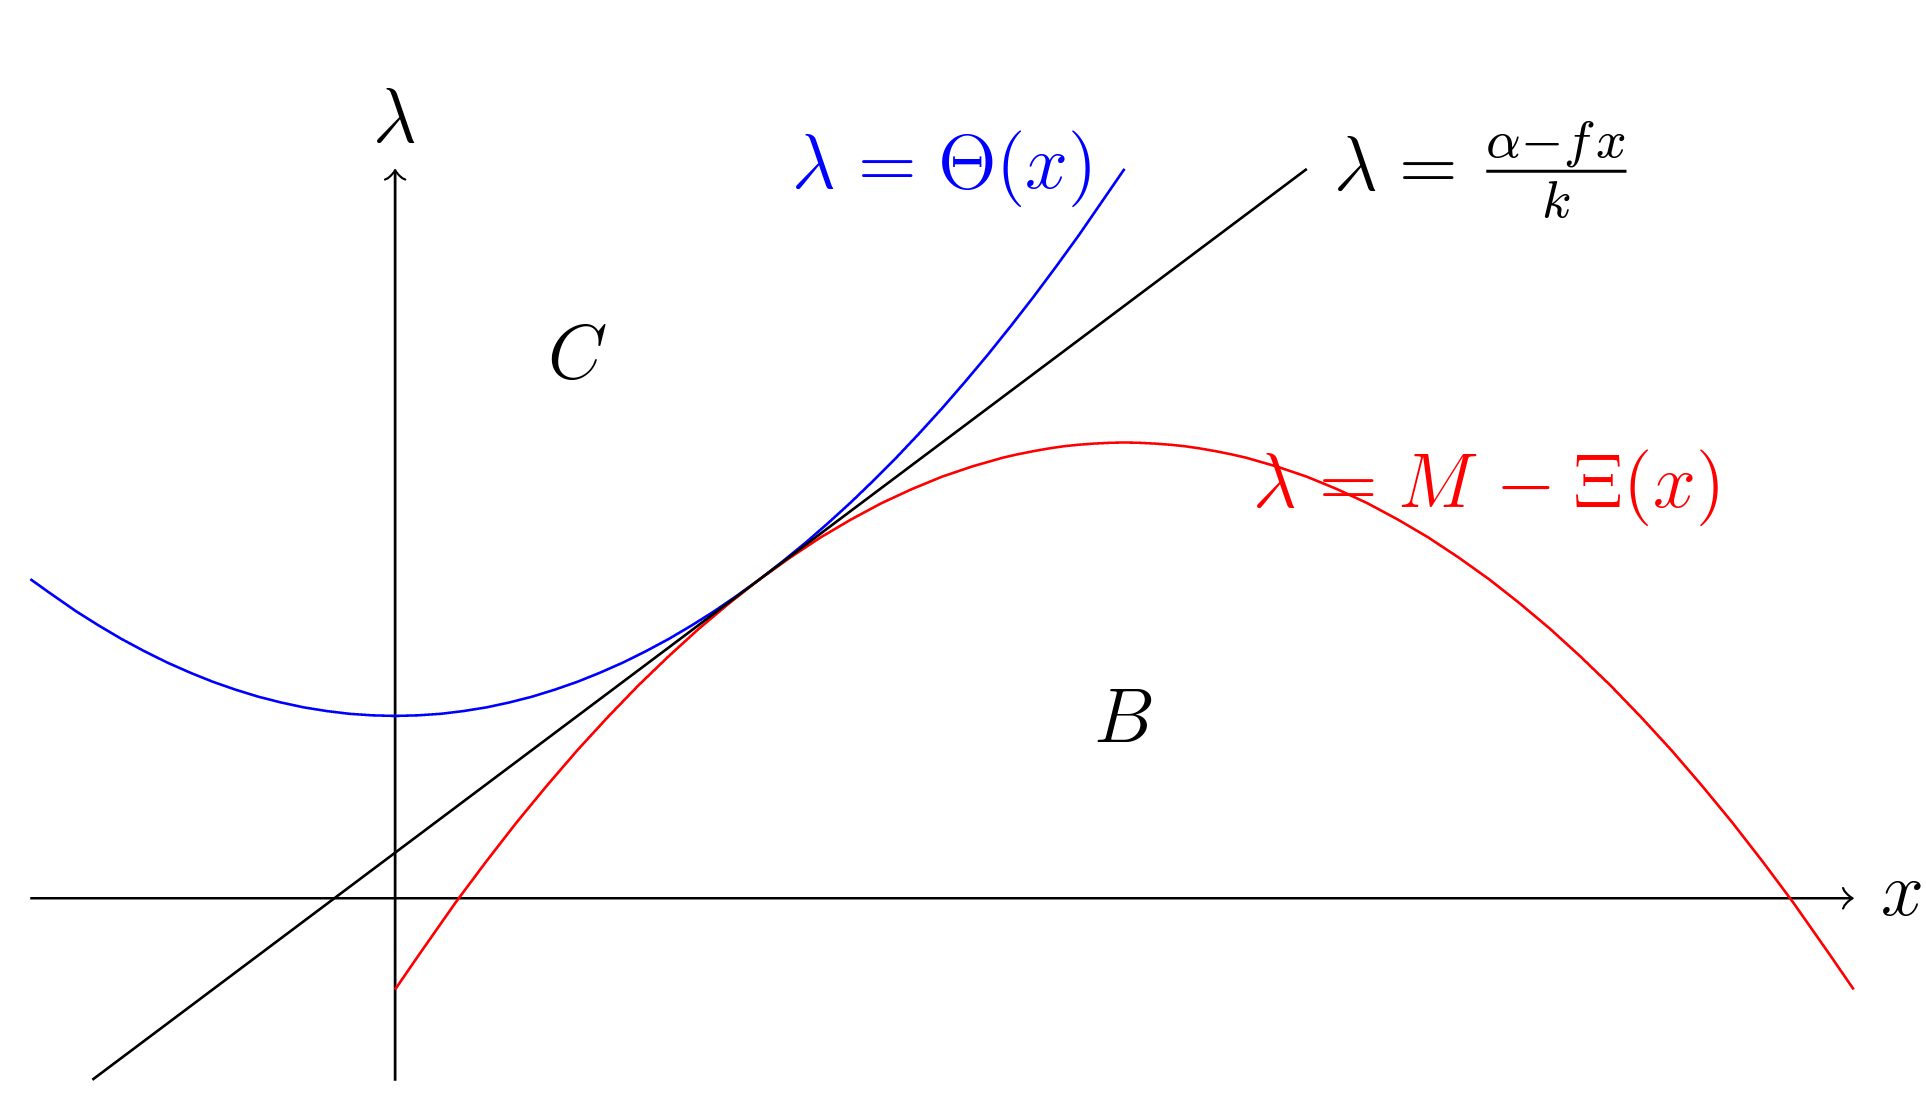
\includegraphics[scale=0.15]{5}
\end{center}
\end{figure}
\s

\newday

(13th February, Wednesday)

\subsection{Proof of Kantorovich Duality}

We first prove that  $\sup \mathbb{J} \leq \inf \mathbb{K}$ (easy part) and $\sup \mathbb{J} \geq \inf \mathbb{K}$ (hard part).
\s

\lemnum{4.7} Under the same conditions as \textbf{Theorem 4.1}, we have
\begin{align*}
\sup_{(\varphi, \psi)\in \Phi_c} \mathbb{J} \leq \inf_{\pi \in \Pi(\mu, \nu)} \mathbb{K}(\pi) 
\end{align*}
\begin{p}
\pf Let $(\varphi, \psi) \in \Phi_c$ and $\pi \in \Pi(\mu, \nu)$. Let $A\subset X$, $B\subset Y$ such that $\mu(A) = 1= \nu(B)$ and $\varphi(x) + \psi(y) \leq c(x,y)$ for all $(x,y)\in A\times B$. Then $\pi(A\times B) =1$(check) hence $\varphi(x) + \psi(y) \leq c(x,y)$ for $\pi$-a.e. $(x,y)$. Then
\begin{align*}
\mathbb{J}(\varphi, \psi) = \int_{X\times Y}(\varphi(x) + \psi(y)) d\pi(x,y) \leq \int_{X\times Y} c(x,y)d\pi(x,y) = \mathbb{K}(\pi)
\end{align*}
Taking supremum over $(\varphi, \psi) \in \Phi_c$ and infimum over $\pi \in \Pi(\mu, \nu)$ gives
\begin{align*}
\sup_{(\varphi, \psi)\in \Phi_c} \mathbb{J} \leq \inf_{\pi \in \Pi(\mu, \nu)} \mathbb{K}(\pi) 
\end{align*}
\eop
\end{p}
\s

\lemnum{4.8} Under the same coditions as \textbf{Theorem 4.1}, has
\begin{align*}
\sup_{(\varphi, \psi)\in \Phi_c} \mathbb{J} \geq \inf_{\pi \in \Pi(\mu, \nu)} \mathbb{K}(\pi) 
\end{align*}
\begin{p}
\pf We prove the lemma when $X$ and $Y$ are compact, and $c$ is continuous. (if not, the proof get much harder)

Let $E= C_b^0 (X\times Y)$ and equip $E$ with the supremum norm. By \emph{Riesz-Markov-Kakutani representation theorem}, has $E^* = \mathscr{M}(X\times Y)$ and the dual pairing
\begin{align*}
\langle \pi, u \rangle = \int_{X\times Y} u(x,y) d\pi(x,y) \quad \text{for } \pi \in E^*, u\in E
\end{align*}
Define
\begin{align*}
& \Theta(u) = \begin{cases}
0 \quad & \text{if } u(x,y) \geq -c(x.y) \,\, \forall x,y\\
+\infty \quad & \text{if otherwise}
\end{cases} \\
& \Xi(u) = \begin{cases}
\mathbb{J}(\varphi, \psi) \quad & \text{if } u(x,y) =\varphi(x) + \psi(y) \,\, \forall x,y\\
+\infty \quad & \text{if otherwise}
\end{cases}
\end{align*}
(Note that $\Xi$ is well-defined even though the representation $u = \varphi \oplus \psi$ is not unique.) Then it is easy to check that $\Theta$ and $\Xi$ are convex.

\quad For $u_0\equiv 1$, then $u_0\geq 0 \geq -c$, so $\Theta(u_0)=0$ and $\Theta$ is continuous at $u_0$ and $\Xi(u_0) =1 < \infty$. So by \emph{Fenchel-Rockafellar Duality},
\begin{align*}
\text{(A)} = \inf_{u\in E}(\Theta(u) + \Xi(u)) = \max_{\pi \in E^*}(-\Theta^*(- \pi)- \Xi^*(\pi)) = \text{(B)}
\end{align*}
Here,
\begin{align*}
\text{(A)} \geq &\inf \big\{\mathbb{J}(\varphi, \psi) : u\geq -c, u = \varphi \oplus \psi, \varphi \in L^1(\mu), \psi \in L^1(\nu) \big\} \\
= & \inf \big\{\mathbb{J}(\varphi, \psi) : \varphi \oplus \psi \geq - c, \varphi \in L^1(\mu), \psi \in L^1(\nu) \big\} \\
= & - \sup_{\Phi_c} \mathbb{J}(\varphi, \psi)
\end{align*}
For (B), 
\begin{align*}
\Theta^*(-\pi) = &\sup_{u\in E}\Big( -\int_{X\times Y} ud\pi - \Theta(u)\Big) = \sup_{u\geq -c, u\in E} \Big( -\int_{X\times Y} y d\pi \Big) \\
=& \sup_{u\leq c, u\in E} \int_{X\times Y} ud\pi = \begin{cases}
\int_{X\times Y} cd\pi \quad &\text{if } \pi \in M_+ \\
+ \infty \quad &\text{if otherwise}
\end{cases}
\end{align*}
and
\begin{align*}
\Xi^*(\pi) =& \sup_{u\in E} \Big( \int_{X\times Y} u d\pi - \Xi(u) \Big) \\
=& \sup_{u\in E, u = \varphi \oplus \psi} \Big( \int_{X\times Y} ud\pi - \int_X \varphi d\mu - \int_Y \psi d\nu \Big) \\
=& \sup_{u\in E, u = \varphi \oplus \psi} \Big( \int_X \varphi(x) d(P^X_{\#}\pi- \mu)(x) + \int_{Y}\psi(y) d(P^{Y}_{\#}\pi - \nu)(y) \Big)\\
=& \begin{cases}
0 \quad & \text{if } \pi \in \Pi(\mu, \nu) \\
+\infty \quad & \text{if otherwise}
\end{cases}
\end{align*}
So
\begin{align*}
\text{(B)} = \max_{\pi \in \Pi(\mu, \nu)} - \mathbb{K}(\pi ) = -\inf_{\pi \in \Pi(\mu, \nu)} \mathbb{K}(\pi)
\end{align*}
So (A)=(B) implies the result.

\eop
\end{p}

\subsection{Existence of Maximisers to the Dual Problem}

The aim here is to find $(\varphi, \psi)$ such that $\sup_{(\varphi, \psi)\in \Phi_c} \mathbb{J}(\varphi, \psi) = \mathbb{J}(\varphi^{\dagger}, \psi^{\dagger})$.

\quad Rather than working with the Legendre-Frenchel transform, it will be more convenient to use the closely related c-transform.
\s

\definum{4.9} For $\varphi : X\rightarrow \bar{\reals} := \reals \cup \{+\infty \}$, $c: X\times Y \rightarrow \reals$, the \textbf{c-transform}, $\varphi^c$ and $\psi^c$ are defined by
\begin{align*}
\varphi^c &: Y\rightarrow \bar{\reals}, \quad y\mapsto \inf_{x\in X} (c(x,y) - \varphi(x)) \\
\varphi^{cc} &: X\rightarrow \reals, \quad x\mapsto \inf_{y\in Y} (c(x,y) -\varphi^c(y))
\end{align*}
If $Y= X^*$ and $c(x,y) = \langle y, x\rangle$ then $(-\varphi)^c (-y) = \varphi^c(y)$.

\quad We can work similarly just using Legendre-Frechel transformation but working just with Legendre-Frenchel transformation makes the problem complicated, and c-transform turns out to have different uses later on.
\s

The main result :
\s

\thmnum{4.10} Let $\mu \in \mathscr{P}(X)$, $\nu\in \mathscr{P}(Y)$, $X,Y$ are Polish spaces and $c: X\times Y\rightarrow [0, +\infty)$. Assume $\exists c_X \in L^1(\mu)$, $c_Y \in L^1(\nu)$ such that $c(x,y) \leq c_X(x) + c_Y(y)$ for $\mu$-a.e. $x\in X$, $\nu$-a.e. $y\in Y$. Then $\exists (\varphi^{\dagger}, \psi^{\dagger}) \in \Phi_c$ such that
\begin{align*}
\sup_{\Phi_c} \mathbb{J}= \mathbb{J}(\varphi^{\dagger}, \psi^{\dagger})
\end{align*}
Furthermore, we can choose $(\varphi^{\dagger},\psi^{\dagger}) = (\eta^{cc}, \eta^c)$ for some $\eta \in L^1(\mu)$.
\s

The existence of $c_X,c_Y$ in the statement of the theorem is effectively a condition on moments, \textit{e.g.} $c(x,y) = |x-y|^2$, then $c(x,y) \leq p|x|^p + p|y|^p$ so $c_X \in L^1(\mu) $ is equivalent to $\int |x|^p d\mu(x) < \infty$.
\s

\newday

(15th February, Friday)
\s

\textbf{Recall :} We defined \textbf{c-trasform} by $\varphi^c(y) = \inf_{x\in X} (c(x,y) - \varphi(x))$. Our goal is to prove \textbf{Theorem 4.10.}
\s

\lemnum{4.11} Let $\mu \in \mathscr{P}(X)$, $\nu \in \mathscr{P}(Y)$, $X, Y$ Polish spaces. For any $a\in \reals$, $(\tilde{\varphi}, \tilde{\psi}) \in \Phi_c$, we have that $(\varphi, \psi) = (\tilde{\varphi}^{cc} - a, \tilde{\varphi}^c + a)$ satisfies $\mathbb{J}(\varphi, \psi) \geq \mathbb{J}(\tilde{\varphi}, \tilde{\psi})$ and $\varphi(x) + \psi(y) \leq c(x,y)$ for $\mu$-a.e. $x\in X$, $\nu$-a.e. $y\in Y$.

\quad Furthurmore, if $\mathbb{J}(\tilde{\varphi}, \tilde{\psi}) > -\infty$ and there are $c_X\in L^1(\mu), c_Y \in L^1(\nu)$ such that $\varphi \leq c_X$ and $\psi \leq c_Y$ then $(\varphi, \psi) \in \Phi_c$.
\begin{p}
\pf Clearly $\mathbb{J}(\varphi -a, \psi +a) = \mathbb{J}(\varphi, \psi)$ for all $a\in \reals$ and for all $\varphi\in L^1(\mu)$, $\psi \in L^1(\nu)$. so it is enoguth to treat the case $a=0$. In fact it is enough to show $\varphi = \tilde{\varphi}^{cc} \geq \tilde{\varphi}$, $\psi = \tilde{\varphi}^c \geq \tilde{\psi}$ and $\varphi(x) + \psi(y) \leq c(x,y)$ 
\begin{i}
\item[1.] $\psi(y) = \inf_{x\in X} (c(x,y)- \tilde{\varphi}(x)) \geq \tilde{\psi}(y)$ using that $\tilde{\varphi} + \tilde{\psi} \leq c(x,y)$
\item[2.] $\varphi(x) = \inf_{y \in Y}(c(x,y) - \tilde{\varphi}^c (y)) = \inf_{y\in Y}\sup_{z\in X}(c(x,y) - c(z,y) + \tilde{\varphi}(z)) \geq \tilde{\varphi}(x)$ by choosing $z=x$.
\item[3.] $\varphi(x) + \psi(y) = \inf_{z\in Y}(c(x,z) - \tilde{\varphi}^c(z) + \tilde{\varphi}^c (y)) \leq c(x,y)$ by choosing $z=y.$.
\end{i}
\s

For the furthermore part, we just need to show $\varphi \in L^1(\mu), \psi\in L^1(\nu)$. Let $M = \int_X c_X(x) d\mu(x)+ \int_Y c_Y(y)d\nu(y) < + \infty$. Note
\begin{align*}
\int_Y (\varphi(x) - c_X(x))d\mu(x) + \int (\psi(y)- c_Y(y)) d\nu(y) = \mathbb{J}(\varphi, \psi) -M \geq \mathbb{J}(\tilde{\varphi}, \tilde{\psi}) - M
\end{align*}
By condition $\varphi \leq c_X$ and $\psi \leq c_Y$, $\int_Y (\varphi(x)- c_X(x))d\mu = - \norms{\varphi - c_X}{L^1(\mu)}$ and $\int (\psi(y)- c_Y(y)) d\nu(y) = -\norms{\psi - c_Y}{L^1(\nu)}$  so this implies
\begin{align*}
\norms{\varphi - c_X}{L^1(\mu)} + \norms{\psi - c_Y}{L^1(\nu)}\leq M - \mathbb{J}(\tilde{\varphi}, \tilde{\psi}) < +\infty
\end{align*}
so
\begin{align*}
\begin{cases}
\varphi - c_X \in L^1(\mu) \\
\psi - c_Y \in L^1(\nu) 
\end{cases} \quad \Rightarrow \quad \begin{cases}
\varphi  \in L^1(\mu) \\
\psi  \in L^1(\nu) 
\end{cases}
\end{align*}
as claimed.

\eop
\end{p}
\s

\lemnum{4.2} Let $\mu \in \mathscr{P}(X)$, $\nu\in \mathscr{P}(Y)$, $X,Y$ Polsih and $c: X\times Y \rightarrow \reals$. Assume $c(x,y) \leq c_X(x) + c_Y(y)$ for functions $c_X\in L^1(\mu) $, $c_Y\in L^1(\nu)$. Then there is a sequence $(\varphi_k, \psi_k)_k \subset \Phi_c$ such that $\mathbb{J}(\varphi_k, \psi_k) \rightarrow \sup_{\Phi_c} \mathbb{J}$ and satisfy $\varphi_k(x) \leq c_X(x)$ for $\mu$-a.e. $x$ and $\psi_k(y) \leq c_Y(y)$ for $\nu$-a.e $y$ for all $k\in \mathbb{N}$.
\begin{p}
\pf Let $(\tilde{\varphi}_k, \tilde{\psi}_k) \in \Phi_c$ be a maximizing sequence. Note $\tilde{\varphi}_k$, $\tilde{\psi}_k$ are proper. Choose
\begin{align*}
a_k = \inf_{y\in Y} \{c_Y(y) - \tilde{\varphi}^c_k (y)\}
\end{align*}
and define $(\varphi_k, \psi_k) = (\tilde{\varphi}^{cc}_k -a_k , \tilde{\varphi}^c_k + a_k)$. If $\varphi_k \leq c_X$ and $\psi_k \leq c_Y$ then by \textbf{Lemma 4.11}, we are done.
\begin{i}
\item[(1)] \textbf{Claim :} $a_k <   + \infty$
\begin{subproof}
: Since $(\tilde{\varphi}_k, \tilde{\psi}_k) \in \Phi_c$, has $\tilde{\varphi}_k(x) \leq c(x,y) - \tilde{\psi}_k(y)$ for $\nu$-a.e. $y\in Y$. Hence $\exists y_0 \in Y$ and $b_0 \in \reals$ such that $\tilde{\varphi}_k(x)\leq c(x, y_0) + b_0$ so $\tilde{\varphi}_k^c(y_0) = \inf_{x\in X} (c(x, y_0) - \tilde{\varphi}_k(x))\geq -b_0$. Hence $a_k \leq c_Y(y_0) - \varphi_c(y_0) \leq c_X(y_0)+b< +\infty$.
\end{subproof}
\item[(2)] \textbf{Claim :} $a_k > - \infty$.
\begin{subproof}
: Has $c_Y(y) - \tilde{\varphi}^c_k(y) = \sup_{x\in X}(c_Y(y) - c(x,y) + \tilde{\varphi}_k(x)) \geq \sup_{x\in X} (-c_X(x) + \tilde{\varphi}_k(x)) \geq -c_X(x_0) + \tilde{\varphi}_k(x_0)$ for all $x_0$. So $a_k \geq \tilde{\varphi}_k(x_0) - c_X(x_0) > -\infty$.
\end{subproof}
\item[(3)] \textbf{Claim :} $\psi_k(y) \leq c_Y(y)$.
\begin{subproof}
: Has $\psi_k(y) = \tilde{\varphi}_k^c (y)+ a_k = \tilde{\varphi}^c_k(y) + \inf_{z\in Y}(c_Y(z)- \tilde{\varphi}^c_k(z)) \leq c_Y(y)$.
\end{subproof}
\item[(4)] \textbf{Claim :} $\varphi_k(x) \leq c_X(x)$.
\begin{subproof}
: Has $\varphi_k(x) - c_X(x) = \inf_{y\in Y} (c(x,y) -\tilde{\varphi}^c_k(y)) - a_k - c_X(x) \leq \inf_{y\in Y}(c_Y(y) - \tilde{\varphi}_k^c(y)) - a_k =0$.
\end{subproof} 
\end{i}
\eop
\end{p}
\s

We now prove the main theorem.
\s

\begin{p}
\textbf{proof of Theorem 4.10)} First note we have
\begin{align*}
\sup_{\varphi, \psi \in \Phi_c}\mathbb{J}(\varphi, \psi) \leq \inf_{\pi \in \Pi(\mu, \nu)} \mathbb{K}(\pi) \leq M := \int c_Xd\mu + \int c_Y d\nu< +\infty
\end{align*}
\quad Let $(\varphi_k, \psi_k) \in \Phi_c$ be maximising sequnce given by \textbf{Lemma 4.12}. Define $\varphi_k^{(l)}$ and $\varphi_k^{(l)}$ by
\begin{align*}
\varphi_k^{(l)}(x) &= \max \{\varphi_k(x) - c_X(x), - l\} + c_X(x) \\
\psi_k^{(l)}(y) &= \max \{ \psi_k(y)- c_y(y) , -l\} + c_Y(y)
\end{align*}
Note
\begin{align*}
\begin{cases}
& \varphi_k \leq \varphi_k^{(l)}, \quad \psi_k \leq \psi_k^{(l)},\\
& -l \leq \varphi_k^{(l)} - c_X(x) \leq 0, \quad  -l \leq \psi_k^{(l)}(y) - c_Y(y)\leq 0\\
& \varphi_k^{(1)}(x) \geq \varphi_k^{(2)}(x) \geq \cdots, \quad \psi_k^{(1)}(x) \geq \psi_k^{(2)}(x) \geq \cdots \\
& \varphi_k^{(l)}(x) + \psi_k^{(l)}(y) \leq \max \{ c(x,y) - c_X(x) - c_Y(y), -l\} + c_X(x) + c_Y(y)
\end{cases}
\end{align*}

\quad For each $l\in \mathbb{N}$, the sequence $\varphi_k^{(l)} - c_X(x)$ is bounded in $L^{\infty}$. So $\varphi_k^{(l)} - c_X(x)$ is bounded in $L^{p}(\mu)$ for all $p\in (1,\infty)$. Since $L^p(\mu)$ is reflexive, we have ``bounded + closed = weakly compact". Hence $\varphi_k^{(l)} -c_X$, upto a subseqeunce, converges weakly in $L^p(\mu)$ as $k\rightarrow \infty$. Since $c_X$ is independent of $k$ then $\varphi_k^{(l)}$, weakly in $L^p(\mu)$.

\quad Choose $p=2$. Then upto a subsequence, for each $l$, has $\varphi_k^{(l)} - c_X \xrightarrow{w} \varphi^{(l)} - c_X \in L^2(\mu) \subset L^1(\mu)$. By a diagonalization argumet, we can assume that $\varphi_k^{(l)} - c_X  \xrightarrow{w} \varphi^{(l)}- c_X$ for all $l\in \mathbb{N}$. Similarly we can choose a subseqeunce with $\psi_k^{(l)} - c_Y\xrightarrow{w} \psi^{(l)} - c_Y \in L^1(\nu)$ for each $l\in \mathbb{N}$ - and furthermore the limit is made pointwise a.e.

\quad Since $c_X\geq \varphi^{(1)} \geq \varphi^{(2)} \geq \cdots$ and $\varphi^{(l)}$, $\psi^{(l)}$ are bounded above by $L^1$ function and monotonically decreasing, we can apply \emph{monotone convergence theorem} to see
\begin{align*}
\lim_{l\rightarrow \infty} \int_X \varphi^{(l)}(x) d\mu(x) = \inf_X \varphi^+(x) d\mu(x), \quad \varphi^+(x) = \lim_{l\rightarrow \infty} \varphi^{(l)}(x) \\
\lim_{l\rightarrow \infty} \int_Y \psi^{(l)}(y) d\nu(x) = \inf_Y \psi^+(y) d\nu(y), \quad \psi^+(y) = \lim_{l\rightarrow \infty} \psi^{(l)}(y) 
\end{align*}

\emph{(needs modification)}
\end{p}
\s

\newday

(18th February, Monday)
\s

\thmnum{4.10} Let $\mu \in \PP(X)$, $\nu \in \PP(Y)$, $X, Y$ Polish space, $c: X\times Y\rightarrow [0, \infty)$. Assume $\exists c_X \in L^1(\mu)$, $c_Y \in L^1(\nu)$ such that $c(x,y)\leq c_X(x) + c_Y(y)$ a.e. Then there is $(\varphi, \psi) \in \Phi_c$ such that $\sup_{\Phi_c} \mathbb{J} = \mathbb{J}(\varphi, \psi)$. Furthermore, we can choose $(\varphi, \psi) = (\eta^{cc}, \eta^c)$ for some $\eta \in L^1(\mu)$.
\begin{p}
\textbf{proof continued)} From last time, we have $(\varphi_k, \psi_k)$ maximising for $\mathbb{J}$. For each $l\in \mathbb{N}$ we found $\varphi_k \leq \varphi_k^{(l)}$, $\psi_k \leq \psi^{(l)}$ such that
\begin{align*}
& \varphi_k^{(l)} + \psi_k^{(l)} \leq \max \{c(x,y) - c_X(x)- c_Y(y), -l \} + c_X(x) + c_Y(y) \call{\oplus} \\
& \varphi_k^{(l)} \xrightarrow{w} \varphi^{(l)}, \quad \psi_k^{(l)} \xrightarrow{w} \psi^{(l)} \quad \text{as } k\rightarrow \infty, \quad \text{in }L^1 \\
& c_x \geq \varphi^{(1)} \geq \varphi^{(2)} \cdots, c_Y \geq \psi^{(1)} \geq \psi^{(2)} \cdots
\end{align*}
Now $\varphi^{(l)}$, $\psi^{(l)}$ are bounded above and monotonically decreasing, so by the monotone convergence theorem,
\begin{align*}
\lim_{l\rightarrow \infty} \int_X \varphi^{(l)}(x) d\mu(x) = \int_X \varphi^{\dagger}(x) d\mu(x), \quad \varphi^{\dagger} = \lim_{l\rightarrow \infty} \varphi^{(l)}(x) \\
\lim_{l\rightarrow \infty} \int_X \psi^{(l)}(x) d\nu(x) = \int_X \psi^{\dagger}(x) d\nu(x), \quad \psi^{\dagger} = \lim_{l\rightarrow \infty} \psi^{(l)}(y)
\end{align*}
\s

We now want to show : (1) $(\varphi^{\dagger}, \psi^{\dagger}) \in \Phi_c$ and (2) $\mathbb{J}(\varphi, \psi) \leq \mathbb{J}(\varphi^{\dagger}. \psi^{\dagger})$ for all $(\varphi, \psi)\in \Phi_c)$.

\quad For (1), letting $l\rightarrow \infty$ in $(\oplus)$,  has $\varphi^{\dagger}(x) + \psi^{\dagger}(y) \leq c(x,y)$. To check integrability, since $\varphi^{\dagger}(x) \leq c_X(x)$, and $\psi^{\dagger}(y) \leq c_Y(y)$ so
\begin{align*}
& - \norms{\psi^{\dagger}- c_X}{L^1(\mu)} - \norms{\psi^{\dagger} - c_Y}{L^1(\nu)} \\
& = \int_X \varphi^{\dagger}(x) - c_X(x) d\mu(x) + \int_Y \psi^{\dagger} (y) - c_Y(y)d\nu(y) \\
& = \mathbb{J}(\varphi^{\dagger}, \psi^{\dagger}) -M
\end{align*}
where $M = \int_X c_X d\mu + \int_Y c_Y d\nu$. So $\norms{\varphi^{\dagger}- c_X}{L^1(\mu)} + \norms{\psi^{\dagger} - c_Y}{L^1(\nu)} \leq M - \mathbb{J}(\varphi^{\dagger}, \psi^{\dagger}) \leq M - \sup_{\Phi_c} \mathbb{J}(\varphi, \psi)$. So $\varphi^{\dagger} \in L^1(\mu)$ and $\psi^{\dagger} \in L^1(\nu)$. Hence $(\varphi^{\dagger}, \psi^{\dagger}) \in \Phi_c$.

\quad For (2),
\begin{align*}
\sup_{\Phi_c} \mathbb{J} =& \lim_{k\rightarrow \infty} \mathbb{J}(\varphi_k, \psi_k) \leq \lim_{k\rightarrow \infty} \mathbb{J}(\varphi_k^{(l)}, \psi_k^{(l)}) \quad \text{for any } l\\
=& \mathbb{J} (\varphi^{(l)}, \psi^{(l)})
\end{align*}
Let $l\rightarrow \infty$, then has
\begin{align*}
\sup_{\Phi_c} \mathbb{J} \leq \lim_{l\rightarrow \infty} \mathbb{J}(\varphi^{(l)}, \psi^{(l)}) = \mathbb{J}(\varphi^{\dagger}, \psi^{\dagger})
\end{align*}
\s

For the furthermore statement, we use the $c$-transform trick as in \textbf{Lemma 4.12} : for all $a\in \reals$, by \textbf{Lemma 4.12},
\begin{align*}
\mathbb{J}(\varphi^{\dagger}, \psi^{\dagger}) \leq \mathbb{J}((\varphi^{\dagger})^{cc} - a, (\varphi^{\dagger})^c +a) = \mathbb{J}((\varphi^{\dagger})^{cc}, (\varphi^{\dagger})^c)
\end{align*}
Let $a= \inf_{y\in Y} (c_Y(y) - (\varphi^{\dagger})^c (y))$, one can show that $a\in \reals$ as in the proof of \textbf{Leamma 4.12}, and $(\varphi^{\dagger})^c(y) + a\leq c_Y(y)$ and $(\varphi^{\dagger})^{cc} (x) - a \leq c_X(x)$. Hence,
\begin{align*}
((\varphi^{\dagger})^{cc} +a, (\varphi^{\dagger})^c -a) \in L^1(\mu) \times L^1(\nu)
\end{align*}
so $((\varphi^{\dagger})^{cc}, (\varphi^{\dagger})^c) \in L^1(\mu) \times L^1(\nu)$.

\eop
\end{p}
\s

\subsection{Kantorovich-Rubinstein Theorem}

\thmnum{4.13} \emph{(Kantorovich-Rubinstein Theorem)} Let $X= Y$ be Polish, $c: X\times Y \rightarrow [0, + \infty]$ be lower semi-continuous metric on $X$. Define $\norms{f}{Lip}= \sup_{x\neq y\in X} \frac{|f(x) - f(y)|}{c(x,y)}$ for $f: X\rightarrow \reals$. Let $\mu \in \PP(X)$, $\nu \in \PP(X)$ and assume $c(\cdot, x_0) \in L^1(\mu)$, $c(x_0, \cdot) \in L^1(\nu)$ for some point $x_0 \in X$. Then
\begin{align*}
\min_{\pi \in \Pi(\mu, \nu)}\mathbb{K}(\pi) = \sup \big\{ \int_X f d(\mu - \nu) : f\in L^1(|\mu - \nu|), \,\, \norms{f}{Lip} \leq 1\big\}
\end{align*}
\begin{p}
\pf We only prove the theorem when $c$ is bounded, \textit{i.e.} $\sup_{x,y\in X} c(x,y) \leq c< + \infty$. So for any $f$ with $\norms{f}{Lip} \leq 1$ we have $|f(x) - f(y) | \leq c$. So $f$ is bounded, and hence we always have $f\in L^1(|\mu - \nu|)$.  By \textbf{Theorem 4.1}, it is enough to check
\begin{align*}
\sup \mathbb{J} = \sup \big\{ \int_X f d(\mu - \nu) : \norms{f}{Lip} \leq 1 \big\}
\end{align*}
From now assume $\forall \eta \in L^1(\mu)$, we have (a) $\snorms{\eta^c}{Lip}\leq 1$, (b) $\eta^{cc} = - \eta^c$ and (c) for all $f$ with $\snorms{f}{Lip} \leq 1$, $(-f, f) \in \Phi_c$.

\quad Assuming (a), (b), (c), by \textbf{Theorem 4.10},
\begin{align*}
\sup_{\Phi_c} \mathbb{J} = & \sup_{\eta \in L^1(\mu)} \mathbb{J}(\eta^{cc}, \eta^c) \\
= & \sup_{\eta \in L^1(\mu)} \mathbb{J}(-\eta^{c}, \eta^c) \quad \text{by assumptoin (b)} \\
\leq & \sup_{\snorms{f}{Lip}\leq 1} \mathbb{J}(-f, f) \quad \text{by assumption (a)} \\
\leq & \sup_{(\varphi, \psi) \in \Phi_c} \mathbb{J}(\varphi, \psi)
\end{align*}
so $\sup_{\Phi_c} \mathbb{J} = \sup_{\snorms{f}{Lip}\leq} \mathbb{J}(f, -f)$ and $\mathbb{J}(f, -f)= \int_X f d(\mu - \nu)$. So the theorem is proved assuming (a), (b), (c).
\s

Now let us justify the assumptions.
\begin{i}
\item[(a)] It is suffiient to show $|\eta^c(x) - \eta^c(y)| \leq c(x,y)$
\begin{align*}
\eta^c (x) - \eta^c(y) =& \sup_{z\in X} \inf_{w\in X}\big( c(x,w) - c(y, z) + \eta(z) - \eta(w) \big) \\
\leq& \sup_{z\in X} \big( c(x,z) - c(y,z) \big) \quad \text{by choosing } w=z \\
\leq& c(x,y) \quad \text{by triangle inequality}  
\end{align*}
By symmetry, $|\eta^c (x) - \eta^c(y)| \leq c(x,y)$ for all $x,y$, so $\norms{\eta^c}{Lip} \leq 1$.
\item[(b)] Has $\eta^{cc}(x) = \inf_{y\in X}(c(x,y) - \eta^c(y)) \leq \eta^c(x)$ since $|\eta^c(y) - \eta^c(x)| \leq c(x,y)$ by (a). On the other hand, again by (a), $\eta^{cc}(x) \geq \inf_{y\in X} (c(x,y) - (\eta^c(x) + c(x,y))) = -\eta^c(x)$ so putting these together, we have $\eta^{cc} = -\eta^c$.
\item[(c)] For all $f$ with $\snorms{f}{Lip}\leq1$, has $f\in L^{\infty}$ so $f\in L^1(\mu) \cap L^1(\nu)$ and by definition of being Lipschitz, 
\begin{align*}
f(x) - f(y) \leq c(x,y)
\end{align*}
so $(f, -f) \in \Phi_c$.
\end{i}

\eop
\end{p}

\newday

(20th February, Wednesday)


\section{Semi-Discrete Optimal Transport}

Assume
\begin{i}
\item[1.] $\nu = \sum_{j=1}^n m_{j} \delta_{y_j}$, $\{m_i\}_{i=1}^n \subset [0,1]$, $\sum_{j=1}^n m_j =1$ and $\{y_j \}_{j=1}^n \subset \reals^d$.
\item[2.] $\mu \in \PP_2(\reals^d)$ has density $\rho$.  
\end{i}
\s

\definum{5.1} The \emph{Laguerre diagram (power diagram)} for a set of points $\{y_j\}_{j=1}^n$ and weight $\{w_j\}_{j=1}^n\subset \reals$ is the collection of sets
\begin{align*}
L_j = \{x\in \reals^d : |x-y|^2 - w_j < |x-y_i|^2 - w_i \,\, \forall i\neq j\}
\end{align*}
for $j=1, \cdots, n$.
\s

\emph{Comments :}
\begin{i}
\item If $w_j =0$, then the \emph{Laguerre diagram} are Voronoi cells.
\item Each $L_i$ is open.
\end{i}
\s

\textbf{Aims :}
\begin{i}
\item Show there exists optimal $T: \reals^d \rightarrow \reals^d$ that defines a Laguerre diagram.
\item and the weights $\{w_j\}_{j=1}^n$ for the optimal Laguerre diagram solve a concave varaiational problem
\begin{align*}
\max g(w) \quad \text{where } w= (w_1, \cdots w_n)
\end{align*} 
where $g$ is as defined in the next lemma.
\end{i}
\s

\lemnum{5.2} Let $\rho \in L^1(\reals^d)$ be a probability density, $\{m_j \}_{j=1}^m \subset [0,1]$ satisfy $\sum_{j=1}^m m_j =1$ and $\{y_j \}_{j=1}^m \subset \reals^d$. Then $g: \reals^n \rightarrow \reals$ defined by 
\begin{align*}
g(w) = \int_{\reals^d} \inf_j (|x-y_j|^2 - w_j) \rho(x) dx + \sum_{j=1}^n w_j m_j \call{\star}
\end{align*}
is concave.
\begin{p}
\textbf{Idea of proof :} Introduce $\gamma : \reals^n \rightarrow \{1, \cdots, n \}$. Define
\begin{align*}
G(\gamma, w) = \int_{\reals^d} \big( |x-y_{\gamma(x)}|^2 - w_{\gamma(x)}\big) \rho(x) dx + \sum_{j=1}^n w_j m_j
\end{align*}
Note (1) $w\mapsto G(\gamma, w)$ is an affine function, so concave and (2) $g(w) = \inf_{\gamma} G(\gamma, w)$. So $g$ is also concave.
\end{p}
\s

\lemnum{5.3} Define $g$ by $(\star)$ for $\rho \in L^1(\reals^d)$, $\{y_j \}_{j=1}^n \subset \reals^n$, $\{m_j \}_{j=1}^n \subset \reals$. Let $\{L_i(w)\}_{i=1}^n$ be a \emph{Laugerre diagram} with weights $w$ and points $\{y_j \}_{j=1}^n$. Then
\begin{align*}
\frac{\pa g}{\pa w_i}(w) = -\int_{L_i(w)} \rho(x) dx + m_i
\end{align*}
\begin{p}
\textbf{sketch proof)} Let $\alpha_j(x, w) = \chi_{L_j(w)}(x) (|x-y_j|^2 -w_j) \rho(x)$ so 
\begin{align*}
g(w) = \sum_{j=1}^n \Big( \int_{\reals^d} \alpha_j(x, w) dx + w_j m_j \Big)
\end{align*} 
For any $x\in L_i(w)$, we have $\chi_{L_i(w + \pm t e_i)} (x) = \chi_{L_j(w)}(x)$ for $t>0$ sufficiently small, where $e_i$ is the unit vector in $i$-direction. Moreover,
\begin{align*}
\frac{1}{t} \big( \alpha_j (x, w+ t e_i) - \alpha_j (x, w) \big) = - \chi_{L_j(w)}(x) \delta_{ij} \rho(x)
\end{align*}
Hence
\begin{align*}
\frac{\pa g}{\pa w_i}(w) = & \lim_{t\rightarrow 0^+} \frac{1}{t} \big( g(w+ t e_i) - g(w) \big) \\
=& \sum_{j=1}^n \lim_{t\rightarrow 0^+} \Big[ \int_{\reals^d} \frac{1}{t} \big( \alpha_j(x, w+ te_i) - \alpha_j(x, w) \big) dx + (w_j + \delta_{ij} t)m_j - w_j m_j \Big] \\
=& -\int_{\reals^d} \chi_{L_i(w)}(x) \rho(x) dx + m_i
\end{align*}
\eop
\end{p}
\s

Then comes the main result of the section.
\s

\thmnum{5.4} Assume $\{y_j \}_{j=1}^m \subset \reals$, $\{m_j\}_{j=1}^m \subset [0,1]$, $\sum_{j=1}^n m_j =1$ and $\nu = \sum_{j=1}^n m_j \delta_{y_j}$. Let $\mu \in \PP_2(\reals^d)$ have density $\rho$ and $g(w)$ is defined by $(\star)$, maximised by $w= (w_1, \cdots, w_n)$, and let $\{L_j\}_{j=1}^n$ be the corresponding \emph{Laguerre diagram}. Now define
\begin{align*}
&T^{\dagger}(x) = y_j \quad \text{if } x\in L_j \quad (\text{which defines }\mu\text{-a.e.}) \\
&\psi^{\dagger}(y_j) = w_j, \quad \varphi^{\dagger}(x) = \inf_{j} (|x-y_j|^2 -w_j)
\end{align*}
Then,
\begin{i}
\item[1.] $T^{\dagger}$ is a solution to the MOT problem with cost $c(x,y) = |x-y|^2$.
\item[2.] $(\varphi^{\dagger}, \psi^{\dagger})$ are an optimal pair for the Kantorovich dual problem with cost $c(x,y) = |x-y|^2$.
\end{i}
\begin{p}
\pf We first assume that $T^{\dagger}$, $\varphi^{\dagger}$ and $\psi^{\dagger}$ are admissible for the optimisation problem:
\begin{subproof}
(a) $\varphi^{\dagger} \in L^1(\mu)$, \quad (b) $T^{\dagger}_{\#}\mu = \nu$, \quad (c) $\int_{L_j} \rho(x)dx = m_j$
\end{subproof}
Assume (a), (b), (c) then
\begin{align*}
\varphi^{\dagger} (x) + \psi^{\dagger} (y_i) = \inf_j \big( |x-y_j|^2 - w_j \big) + w_i \leq |x-y_i|^2 = c(x, y_i)
\end{align*}
So $(\varphi^{\dagger}, \psi^{\dagger}) \in \Phi_c$. Now we have
\begin{align*}
\begin{array}{rl}
\mathbb{M}(T^{\dagger}) \geq & \inf_{T_{\#} \mu = \nu} \mathbb{M}(T) \quad (\text{by (b)}) \\
\geq & \min_{\pi \in \Pi(\mu, \nu)} \mathbb{K}(\pi) \\
= & \sup_{(\varphi, \psi)\in \Phi)c} \mathbb{J}(\varphi, \psi) \quad \text{by Theorem 4.1}\\
\geq & \mathbb (\varphi^{\dagger}, \psi^{\dagger}) 
\end{array}  \call{\oplus}
\end{align*}
and
\begin{align*}
\mathbb{J} (\varphi^{\dagger}, \psi^{\dagger}) =& \int_{\reals^d} \varphi^{\dagger} (x) \rho(x) dx + \sum_{j=1}^n m_j \psi^{\dagger}(y) \\
=& \sum_{j=1}^n \Big( \int_{L_j} \varphi^{\dagger} (x) \rho(x) dx + m_j \psi^{\dagger}(y_j) \Big) \\
=& \sum_{j=1}^n \int_{L_j} \Big( \big( |x-y_j|^2 - w_j \big) \rho(x) dx + m_j w_j \Big) \\
=& \sum_{j=1}^n \int_{L_j} |x- y_j|^2 \rho(x) dx \\
=& \sum_{j=1}^n \int_{L-j} |x- T^{\dagger}(x)|^2 \rho(x) dx = \mathbb{M}(T^{\dagger})
\end{align*}
Hence all inequalities in $(\oplus)$ are all equalities and in particular
\begin{align*}
\mathbb{M}(T^{\dagger}) & =\min_{T: T_{\#} \mu = \nu} \mathbb{M}(T) \\
\mathbb{J}(\varphi^{\dagger}, \psi^{\dagger}) & = \sup_{(\varphi, \psi) \in \Phi_c} \mathbb{J}(\varphi, \psi)
\end{align*}
\s

Now we are left to prove assumptions (a), (b), (c).
\begin{i}
\item[(a)] Has
\begin{align*}
-\sup_{j} w_j \leq \varphi^{\dagger}(x) \leq |x- y_i|^2 - w_i
\end{align*}
for any $i$ so $|\varphi^{\dagger}(x)| \leq 2|x|^2 + C$ for a constant $C= 2|y_1|^2 - w_1 + \sup_j w_j$ and
\begin{align*}
\norms{\varphi}{L^1(\mu)} \leq 2\int_{\reals^d} |x|^2 d\mu(x) + C < + \infty
\end{align*}
\item[(b)] Pick $i\in \{1, \cdots, n\}$. Then
\begin{align*}
\mu((T^{\dagger})^{-1} (y_i)) =& \mu(\{x: T^{\dagger}(x) = y_i \}) = \mu(L_i) = m_i \quad (\text{by (c)}) \\
=& \nu(\{y_i\})
\end{align*}
So $T^{\dagger}_{\#} \mu = \nu$ as required.
\item[(c)] Since $w$ maximises $g$, has $\frac{\pa g}{\pa w_i}(w) =0$ for each $i$, but $\frac{\pa g}{\pa w_i}(w) = - \int_{L_j} \rho(x) dx + m_j$ by \textbf{Lemma 5.3} so we have the result
\end{i} 
\eop
\end{p}
\s

\newday

(22nd February, Friday)
\s

\textbf{A proof for yesterday Example Class :} when showing $\sup_{Ax\leq b} c\cdot x = \min_{y\geq 0, A^T y =c} b\cdot y$. We first assume that $\exists y_0$ such that $y_0 \geq A^T y_0 =c$ (if not, can just define that the minimum takes value $\infty$)
\s

Correction 1 : We defined $\Xi(x) = c\cdot x$, $\Xi : E\rightarrow \reals$ by $A^T y_0 \cdot x = y_0 \cdot (Ax)$ so $\Xi$ is indeed well-defined.

Correction 2 : We should have $E^* \cong \text{Range}(A) \subset \reals^m$.
\s

\section{Existence and Characterisation of Transport Maps}

Aims in this chapter are the following.
\begin{i}
\item[(1)] To find a sufficient condition for the existence of Optimal Transport mapos for the MOT problem.
\item[(2)] To find a sufficient condition for the Monge cost to equal the Kantorovich cost.
\item[(3)] To characterise Optimal Transport maps and plans.
\end{i}
The structure would look like
\begin{i}
\item[6.1] Sate main results
\item[6.2] Background on convex analysis
\item[6.3] Prove main results
\end{i}

\subsection{Knott-Smith Optimality and Beiner's Theorem}

\defi The \textbf{subdifferential} of a convex function $\varphi$ is defined to be
\begin{align*}
\pa \varphi(z) = \{y : \varphi(z) \geq \varphi(x) + y\cdot (z-x) \quad \forall z\in \reals^d \}
\end{align*}
This is a \emph{set of slopes}.
\s

\emph{Comments :}
\begin{i}
\item[(1)] Subdifferential always exists for convex lower semi-continuous functions.
\item[(2)] if $\varphi$ is differentiable at $x$, then $\pa \varphi(x) = \{ \nabla \varphi(x) \}$.
\end{i}
\s

\thmnum{6.1} \emph{(Knott-Simith Optimality Criterion)} Let $\mu \in \mathscr{P}_2(X)$, $\nu \in \mathscr{P}_2(Y)$, $X, Y \subset \reals^d$, $c(x,y)= \frac{1}{2}|x-y|^2$. Then $\pi^{\dagger} \in \Pi(\mu, \nu)$ minimisies the KOT problem \emph{iff} $\exists \tilde{\varphi}^{\dagger} \in L^1(\mu)$ convex and lower semi-continuous such that $\text{supp}(\pi^{\dagger}) \subset \text{Gra}( \pa \tilde{\varphi}^{\dagger})$ (equivalent to having $y\in \pa \tilde{\varphi}^{\dagger}(x)$ for $\pi^{\dagger}$-a.e. $(x,y)$). Moreover the pair $(\tilde{\varphi}^{\dagger}, (\tilde{\varphi}^{\dagger})^c)$ is a minimiser of $\inf_{\tilde{\Phi}} \mathbb{J}$, where $\tilde{\Phi} = \{ (\tilde{\varphi}, \tilde{\psi}) \in L^1(\mu)\times L^1(\nu) : \tilde{\varphi}(x) + \tilde{\psi}(y) \geq x\cdot y \}$.
\s

(Previously, $\sup_{(\varphi, \psi) \in \Phi} \mathbb{J}(\varphi, \psi)$ was the dual problem. Here we are interested in the probelms $\inf_{(\tilde{\varphi}, \tilde{\psi}) \in \tilde{\Phi}} \mathbb{J}(\tilde{\varphi}, \tilde{\psi})$. The two problems can be related by : $(\tilde{\varphi}, \tilde{\psi}) \in \tilde{\Phi}$ minimises $\mathbb{J}$ over $\tilde{\Phi}$ \emph{iff} $(\varphi, \psi) \in \Phi$ maximises $\mathbb{J}$ over $\Phi$ where $\tilde{\varphi}(x) = \frac{1}{2} |x|^2 - \varphi(x)$, $\tilde{\psi}(y) = \frac{1}{2} |y|^2 - \psi(y)$.)
\s

In 1D we expect monotonicity, and the theorem is almost equivalent to monotonicity : if $x_1 \leq x_2$ then $T^{\dagger}(x_1) \leq T^{\dagger}(x_2)$. Hence $\text{supp}(\pi^{\dagger}) = \{(x,y) : x\in X, y= T(x)\}$ is \textbf{cyclically monotone} - if $(x_1, y_1), (x_2, y_2) \in \text{supp}(\pi^{\dagger})$ and $x_1\leq x_2$ then $y_1 \leq y_2$. Any cyclically monotone set can be written as a subdifferential of a convex function. This argument holds for higher dimensions and if $T$ is ``set valued".
\s

\thmnum{6.2} \emph{(Brenier's Theorem)} Let $\mu \in \mathscr{P}_2(X)$, $\nu \in \mathscr{P}_2(Y)$, $X, Y\subset \reals^d$ and $c(x,y) = \frac{1}{2} |x-y|^2$. Assume that $\mu$ does not give mass to small sets (a small set is any set with Hausdorff dimenstion at most $d-1$). Then there is a unique $\pi^{\dagger} \in \Pi(\mu, \nu)$ that minimises the KOT problem.

\quad Moreover, $\pi^{\dagger}$ satisfies $\pi^{\dagger} = (id \times \nabla \tilde{\varphi})_{\#} \mu$ where $\nabla \tilde{\varphi}$ is the unique gradient of a convex function that pushes $\mu$ forward to $\nu$ (that is, $(\nabla \tilde{\varphi})_{\#} \mu = \nu$) and $(\tilde{\varphi},\tilde{\varphi}^c)$ minimise $\mathbb{J}$ over $\tilde{\Phi}$.
\s

\emph{Comments :}
\begin{i}
\item[(1)] $\pi^{\dagger} = (id \times \nabla \tilde{\varphi})_{\#} \mu$ $\Leftrightarrow$ $d\pi^{\dagger}(x,y) = \delta_{\nabla \tilde{\varphi}(x)}(y) \times d\mu(x)$.
\item[(2)] We will show that, in \textbf{Proposition 6.5}, convex functions are differentiable Lebesgue almost everywhere. Since $\mu$ gives zero mass to ses of Lebesue measure 0, then any convex function is differentiable $\mu$ almost everywhere.
\end{i}
\s

\corrnum{6.3} Under the same assumptions as \textbf{Theorem 6.2}, $\nabla \tilde{\varphi}$ is the unique solution to the MOT problem, \textit{i.e.}
\begin{align*}
\frac{1}{2} \int_X |x- \nabla \tilde{\varphi}(x)|^2 d\mu(x) = \inf_{T: T_{\#}\mu = \nu} \frac{1}{2} \int_X |x- T(x)|^2 d\mu(x)
\end{align*}
\begin{p}
\pf Since $\min \mathbb{K} \leq \inf \mathbb{M}$, and $T^{\dagger}_{\#} \mu = \nu$ by \textbf{Theorem 6.2}, it is enough to show that $T^{\dagger} = \nabla \tilde{\varphi}$ satisfies $\mathbb{M}(T^{\dagger}) = \min \mathbb{K} = \mathbb{K}(\pi^{\dagger})$. Indeed,
\begin{align*}
\mathbb{M}(T^{\dagger}) =& \frac{1}{2} \int_X |x-T^{\dagger}(x)|^2 d\mu(x) \\
=& \frac{1}{2} \int_{X\times Y} |x- T^{\dagger}(x)|^2 d\pi^{\dagger}(x,y) \\
=& \frac{1}{2} \int_{X\times Y} |x-y|^2 d\pi^{\dagger} (x,y) \quad (\text{since } y =T^{\dagger}(x),\,\, \pi^{\dagger}\text{-a.e.}) \\
=& \mathbb{K}(\pi^{\dagger})
\end{align*}
\eop
\end{p}

\subsection{Preliminary Results for Convex Analysis}

Just in this seciton, we will write $\varphi$ rather than $\tilde{\varphi}$.
\s

Recall the \emph{Legendre-Fenchel transform}, or the convex conjugate defined by
\begin{align*}
\varphi^*(y) = \sup_{x\in \reals^d} (x\cdot y - \varphi(x))
\end{align*}
\s

\propnum{6.4} Let $\varphi : \reals^d \rightarrow \reals\cup \{\infty\}$ be proper (not identically $+ \infty$), lower semi-continuous and convex fuction. Then $\forall x, y\in \reals^d$, 
\begin{align*}
xy = \varphi(x) + \varphi^*(y) \quad \Leftrightarrow \quad y\in \pa \varphi(x)
\end{align*}
\begin{p}
\pf Note, by definition, $\varphi^*(y) \geq x\cdot y - \varphi(x)$ for all $x\in \reals^d$. So
\begin{align*}
x\cdot y= \varphi(x) + \varphi^*(y) \quad \Leftrightarrow & \quad x\cdot y \geq \varphi(x) + \varphi^*(y) \\
\Leftrightarrow & \quad x\cdot y \geq \varphi(x) + y\cdot z - \varphi(z) \quad \forall z\in \reals^d \\
\Leftrightarrow & \quad \varphi(z) \geq \varphi(x) + y\cdot(z-x) \quad \forall z\in \reals^d \\
\Leftrightarrow & \quad y\in \pa \varphi(x)
\end{align*}
\eop
\end{p}
\s

\propnum{6.5} Let $\varphi : \reals^d \rightarrow \reals \cup \{+\infty \}$ be convex, then
\begin{i}
\item[(1)] $\varphi$ is differential Lebesgue-almost everywhere on the interior of its domain and
\item[(2)] Whenever $\varphi$ is differentiable, has $\pa \varphi(x) = \{\nabla \varphi(x) \}$.
\end{i}
\s

\newday

(25th February, Monday)
\s

We use the following theorem for the proof.
\s

\statement{Rademacher's Theorem} If $U\subset \reals^d$ is open and $f:U\rightarrow \reals$ is Lipschitz continuous then $f$ is differentiable a.e.

\quad We do not prove this results.
\s

\propnum{6.5} Let $\varphi : \reals^d \rightarrow \reals \cup \{+\infty \}$ be convex, then
\begin{i}
\item[(1)] $\varphi$ is differential Lebesgue-almost everywhere on the interior of its domain and
\item[(2)] Whenever $\varphi$ is differentiable, has $\pa \varphi(x) = \{\nabla \varphi(x) \}$.
\end{i}
\begin{p}
\pf \begin{i}
\item[(1)] Let $x\in \text{int}(\text{Dom}(\varphi))$ and $\delta^*$ be such that $\overline{B(x, \delta^*)} \subset \text{int}(\text{Dom}(\varphi))$. We show that $\varphi$ is Lipschitz continuous on $B(x, \delta^*/4)$. Then by \emph{Rademacher's Theorem}, $\varphi$ is a.e. differentiable in $B(x, \delta^*/4)$. Then $\varphi$ is differentiable a.e. on $\text{int}(\text{Dom}(\varphi))$.

(a) We show $\varphi$ is uniformly bounded on $\overline{B(x, \delta^*/2)}$. Let $Q$ be a cuboid centred at $x$ with sides of legth $\sqrt{\frac{4}{d}} \delta^*$. Let $\{x_i\}_{i=1}^n$ be the corners of $Q$. Note $x\in \pa B(x, \delta^*)$ and that the set of exterme points of $Q$ is $\{x_i \}_{i=1}^d$. by the \emph{Minkowski-Careth\'{e}odory theorem} (Theorem 3.5), for each $y \in \overline{B(x, \delta^*/\sqrt{d})}$, $\exists \{\lambda_i \}_{i=1}^{2^d} \subset [0,1]$ such that $\sum_{i=1}^{2^n} \lambda_i =1$ and $y = \sum_{i=1}^{2^d} \lambda_i x_i$. So
\begin{align*}
\varphi(y) = \varphi \big( \sum_{i=1}^{2^d} \lambda_i x_i \big) \leq \sum_{i=1}^{2^d} \lambda_i \varphi(x_i) \leq \max_{i} |\varphi(x_i)| =C
\end{align*}
where the first inequality follows from convexity of $\varphi$. Now define $y' = (x-(y-x)) = 2x-y \in B(x, \delta^*/2)$. Since $x= \frac{1}{2} y' + \frac{1}{2}y$, has
\begin{align*}
& \varphi(y) \geq 2\varphi(x) - \varphi(y') \geq 2\varphi(x) - C  \\
\Rightarrow \quad & 2\varphi(x) - C \leq \varphi(y) \leq C, \quad \forall y\in \overline{B(x, \delta^*/\sqrt{d} )}
\end{align*}
so 
\begin{align*}
\norms{\varphi}{L^{\infty}(\overline{B(x, \delta^*/\sqrt{d})})} \leq \max \{C- 2\varphi(x), C\} = M < \infty
\end{align*}

(b) We show $\varphi$ is Lipschitz continuous on $B(x, \delta^*/2\sqrt{d})$. Let $x_1, x_2 \in B(x, \delta^*/2\sqrt{d})$ where $x_1 \neq x_2$. Take $x_3$ to be the intersectin of the line throgh $x_1$ and $x_2$ with $\pa B(x, \delta^*/\sqrt{d})$ and choose $x_3$ such that $x_2$ lies between $x_1$ and $x_3$. Define $\lambda = \frac{|x_2 - x_3|}{|x_1 -x_3|} \in (0,1)$. Now,
\begin{align*}
\lambda x_1 + (1- \lambda) x_3 =& \lambda x_2 + \lambda( x_1 - x_2) + (1- \lambda )x_2 + (1- \lambda)(x_3 - x_2) \\
=& x_2 + \frac{|x_2 -x_3|}{|x_1 -x_3|} (x_1 -x_2) + \frac{|x_1- x_3| - |x_2 -x_3|}{|x_2 - x_3|}(x_3 -x_2) \\
=& x_2 + \frac{1}{|x_1-x_3|} \big( |x_2 - x_3| (x_1-x_2) + |x_1 - x_2|(x_3 -x_2) \big) \\
=& x_2
\end{align*}
By convexity of $\varphi$,
\begin{align*}
\varphi(x_2) & \leq (1- \lambda) \varphi(x_3) + \lambda \varphi(x_1) \\
\Rightarrow \quad  \varphi(x_2) - \varphi(x_1) &\leq (1- \lambda)(\varphi(x_3) - \varphi(x_1)) = \frac{|x_1 -x_2|}{|x_1 -x_3|}(\varphi(x_3) - \varphi(x_1)) \\
& \leq \frac{2\sqrt{d}\times 2M}{\delta^*}|x_1 -x_2| = L|x_1 -x_2|
\end{align*}
with $L = 4\sqrt{d}M/ \delta^*$. So $\varphi$ is Lipschitz. \emph{[This proof looks very complicated but the idea is very simple!]}

\item[(2)] Let $\varphi$ be differentiable at $x$. Then
\begin{align*}
\varphi(x) + \nabla \varphi(x) \cdot (z-x) =& \varphi(x) + \lim_{h\rightarrow 0^+} \Big( \frac{\varphi(x + (z-x)h) - \varphi (x)}{h} \Big) \\
=& \varphi(x) + \lim_{h\rightarrow 0^+} \Big( \frac{\varphi((1-h)x + zh) - \varphi (x)}{h} \Big) \\
\leq & \varphi(x) + \lim_{h\rightarrow 0} \frac{(1-h)\varphi(x) + h\varphi(z) - \varphi(x)}{h} =\varphi(z) 
\end{align*}
so $\nabla \varphi(x) \in \pa \varphi(x)$.

\quad On the other hand, if $y\in \pa \varphi(x)$, then $\varphi(x) + y\cdot(z-x) \leq \varphi(x)$ for all $z\in \reals^d$ so by letting $z= x+ hw$ with $h>0$, we get
\begin{align*}
y\cdot w \leq \frac{\varphi(x+ hw) - \varphi(x)}{h}
\end{align*}
Let $h\rightarrow 0^+$, then $y\cdot w \leq \nabla \varphi(x) \cdot w$. By symmetry ($w\mapsto -w$), we also have $y\cdot w = \nabla \varphi(x) \cdot w$ for all $w\in \reals^d$. Hence $y= \nabla \varphi(x)$.
\end{i}
\eop
\end{p}
\s

\propnum{6.6} Let $\varphi : \reals \cup \{+\infty \}$ be proper. then the following are equivalent.
\begin{i}
\item[(1)] $\varphi$ is convex and lower semi-continuous.
\item[(2)] $\varphi = \psi^*$ for some proper function $\psi$.
\item[(3)] $\varphi^{**} = \varphi$.
\end{i}
\begin{p}
\pf The implications from (3) to (2) is immediate.

\quad We are left to show implication $(2)\, \Rightarrow \,(1)$. Assume (2), so $\varphi = \psi^*$ for some proper function $\psi$. Let $x_1, x_2\in \reals^d$, $t\in [0,1]$, then 
\begin{align*}
\varphi(tx_1 + (1-t)x_2) & = \sup_y \big( (tx_1 +(1-t)x_2)\cdot y - \psi(y) \big) \\
& \leq \sup_y \big( t(x_1 \cdot y) - \psi(y) \big) + \sup_y \big((1-t)(x_2 \cdot y - \psi(y) \big) \\
& = t\varphi(x_1) + (1-t) \varphi(x_2)
\end{align*}  
so $\varphi$ is convex. To show lower semi-continuity, let $x_m \rightarrow x$. Then
\begin{align*}
\liminf_{m\rightarrow \infty} \varphi(x_m) =& \liminf_{m\rightarrow \infty} \sup_y (x_m \cdot y -\psi(y)) \geq \lim_{m\rightarrow \infty} (x_m \cdot y - \psi(y)) \\
=& x\cdot y - \psi(y) \quad \text{for any } y\in \reals^d
\end{align*}
so $\liminf_{m\rightarrow \infty} \varphi(x_m) \geq \sup_y (x\cdot y - \psi(y)) = \varphi(x)$, so $\varphi$ is lower semi-continuous.
\end{p}
\s

\newday

(27th February, Wednesday)
\s

\begin{p}
\textbf{proof continued)} Next we prove implication (1) to (3). Suppose $\varphi$ is convex and lower semi-continuous. Assume $x\in \text{int}(\text{Dom}(\varphi))$ and we show $\varphi^{**}(x) = \varphi(x)$. Since $\varphi$ can be bounded below by an affine function passing through $(x, \varphi(x))$, we have $\pa \varphi(x) \neq \phi$. Let $y_0 \in \pa \varphi(x)$. By $\textbf{Proposition 6.4}$, $x\cdot y_0 = \varphi(x) + \varphi^*(y_0)$, so
\begin{align*}
\varphi(x) = x\cdot y_0 - \varphi^*(y_0) \leq \sup_{y\in \reals^n} (x\cdot y - \varphi^c(y)) =  \varphi^{**}(x)
\end{align*}
On the other hand, since $\varphi^*(y) \geq x\cdot y - \varphi(x)$ for all $y\in \reals^d$, has 
\begin{align*}
\varphi(x) \geq \sup_y (x\cdot y - \varphi^*(y)) = \varphi^{**}(x)
\end{align*}
so $\varphi(x) = \varphi^{**}(x)$ on $\text{int}(\text{Dom}(\varphi))$. See note for the case $x\not\in \text{int}(\text{Dom}(\varphi))$.

\eop
\end{p}

\subsection{Proof of the Knott-Smith Optimality Criterion}

Let $c(x,y) = \frac{1}{2} |x-y|^2$, $\mu, \nu \in \mathscr{P}_2 (\reals^d)$. We first make few observations. 
\begin{i}
\item[(A)] Let $(\varphi, \psi) \in \Phi_c$. Define $\tilde{\varphi}(x) = \frac{1}{2} |x|^2 - \varphi(x)$ and $\tilde{\psi}(y) = \frac{1}{2} |y|^2 - \psi(y)$. One can see that $\tilde{\varphi} \in L^1(\mu)$, $\tilde{\psi} \in L^1(\nu)$. and 
\begin{align*}
\tilde{\varphi}(x) + \tilde{\psi}(y) =& \frac{1}{2} |x|^2 + \frac{1}{2} |y|^2 - \varphi(x) - \varphi(y) \\
\geq & \frac{1}{2} |x|^2 + \frac{1}{2} |y|^2 - \frac{1}{2} |x-y|^2 = x\cdot y
\end{align*}
So $(\tilde{\varphi}, \tilde{\psi}) \in \tilde{\Phi}$ where $\tilde{\Phi} = \{(\tilde{\varphi}, \tilde{\psi}) \in L^1(\mu) \times L^1(\nu) : \tilde{\varphi}(x) + \tilde{\psi}(y) \geq x\cdot y\}$.

\quad Similarly if $(\tilde{\varphi}, \tilde{\psi}) \in \tilde{\Phi}$, then $(\varphi, \psi) \in \Phi_c$.

\item[(B)] If we let $M = \frac{1}{2}\int_X |x|^2 d\mu(x) + \frac{1}{2} \int_Y |y|^2 d\nu(y)$, then $\mathbb{J}(\tilde{\varphi}, \tilde{\psi}) = M - \mathbb{J}(\varphi, \psi)$ and for $\pi \in \Pi(\mu, \nu)$, has $\mathbb{K}(\pi) = M - \int_{X\times Y} x\cdot y d\pi(x,y)$. Kantorovich duality (\textbf{Theorem 4.1}) implies that
\begin{align*}
\min_{(\tilde{\varphi}, \tilde{\psi}) \in \tilde{\Phi}} \mathbb{J}(\tilde{\varphi}, \tilde{\psi})  = \max_{\pi \in \Pi(\mu, \nu)} \int_{X\times Y} x\cdot y d\pi(x,y)
\end{align*}
Also 
\begin{align*}
\pi^{\dagger} \in \Pi(\mu, \nu)\text{ minimises }\mathbb{K}\text{ over }\Pi(\mu, \nu) \,\, &\Leftrightarrow \,\, \pi^{\dagger}\text{ maximises }\int_{X\times Y} x\cdot y d\pi(x,y) \\
(\varphi, \psi) \in \Phi_c\text{ maximises }\mathbb{J}\text{ over }\Phi_c \,\, & \Leftrightarrow \,\,(\tilde{\varphi}, \tilde{\psi}) \in \tilde{\Phi}\text{ minimise }\mathbb{J}\text{ over }\tilde{\Phi}.
\end{align*}

\item[(C)] Recall that there exists maximiser $(\varphi^{cc}, \varphi^c)\in \Phi_c$ of $\mathbb{J}$. So $(\tilde{\varphi}, \tilde{\psi}) := (\frac{1}{2}|\cdot|^2 - \varphi^{cc}, \frac{1}{2}|\cdot|^2 - \varphi^c)$ minimise $\mathbb{J}$ over $\tilde{\Phi}$. Furthermore
\begin{align*}
\tilde{\psi}(y) =& \frac{1}{2}|y|^2 - \varphi^c(y) = \sup_{x\in X} \big( \frac{1}{2} |y|^2 - \frac{1}{2}|x-y|^2 + \varphi(y) \big) \\
=& \sup_{x\in X} \big( x\cdot y -\frac{1}{2} |x|^2 + \varphi(x) \big) = \sup_{x\in X} (x\cdot y - \tilde{\varphi}(x)) = \tilde{\varphi}^*(y)
\end{align*}
And
\begin{align*}
\tilde{\varphi}(x) =& \frac{1}{2} |x|^2 - \varphi^{cc}(x) = \sup_{y\in Y} \big( \frac{1}{2} |x|^2 - \frac{1}{2} |x-y|^2 + \varphi^c (y) \big) \\
=& \sup_{y\in Y}\big( \frac{1}{2}|x|^2 - \frac{1}{2}|x-y|^2 + \frac{1}{2}|y|^2 - \tilde{\varphi}^*(y) \big) \quad (\text{used previous computation}) \\
=& \sup_{y\in Y} (x\cdot y - \tilde{\varphi}^*(y)) \\
=& \tilde{\varphi}^{**}(x)
\end{align*}
By \textbf{Proposition 6.6}, $\tilde{\eta} := \tilde{\varphi}^{**}$ is convex and lower semi-continuous and $\tilde{\eta}^* = \tilde{\varphi}^{***} = \tilde{\varphi}^*$. 
\item[(D)] For $(\tilde{\varphi}, \tilde{\varphi}^*)$ with $\tilde{\varphi} \in L^1(\mu)$, we have
\begin{align*}
\int_{X\times Y} \tilde{\varphi}(x) + \tilde{\varphi}^* (y) d\pi^{\dagger}(x,y) & = \int_{X\times Y} x\cdot y d\pi^{\dagger}(x,y) \\
& \leq \frac{1}{2} \int_{X\times Y} |x|^2 + |y|^2 d\pi^{\dagger} (x,) =\frac{1}{2} \int_X |x|^2 d\mu(x) + \frac{1}{2} \int_Y |y|^2 d\nu(y)
\end{align*}
so $\mathbb{J}(\tilde{\varphi}, \tilde{\varphi}^*) < \infty$.
\item[(E)] From the result of (C), if we just prove that $\tilde{\varphi}^* \in L^1(\nu)$ whenever $\tilde{\varphi} \in L^1(\mu)$, then $(\eta, \eta^*) \in L^1(\mu) \times L^1(\nu)$ so there is a minimiser of $\mathbb{J}$ and $\tilde{\Phi}$ that takes the form $(\tilde{\eta}, \tilde{\eta}^*)$ where $\tilde{\eta}$ is convex, lower semi-continuous and is proper.
\s

To see this, assume $\tilde{\varphi}\in L^1(\mu)$. First note that $\exists x_0 \in X$ and $b_0 = \tilde{\varphi}(x_0) +1 \in \reals$ such that
\begin{align*}
\tilde{\varphi}^*(y) \geq x_0 \cdot y - \tilde{\varphi}(x_0) -1 =: x_0 \cdot y - b_0 =: f(y)
\end{align*} 
Then we have $\tilde{\varphi}^* - f(y) \geq 0$, so $\norms{\tilde{\varphi}^* - f}{L^1(\mu)} = \int_Y \big( \tilde{\varphi}^*(y) - f(y) \big) d\nu(y)$. Hence
\begin{align*}
\norms{\tilde{\varphi}^* - f}{L^1(\mu)} =& \int_Y \big( \tilde{\varphi}^*(y) - f(y) \big) d\nu(y) \\
\leq & \, \mathbb{J} (\tilde{\varphi}, \tilde{\varphi}^*) + \norms{\tilde{\varphi}}{L^1(\mu)} + \frac{1}{2} |x_0| + \frac{1}{2} \int_Y |y|^2 d\nu(y) + b_0 \\
<&  +\infty
\end{align*}
where the second line is implied by Cauchy-Schwarz ienquality. So $\tilde{\varphi}^* - f\in L^1(\nu)$ and since $f\in L^1(\nu)$, we conclude $\tilde{\varphi}^* \in L^1(\nu)$ as required.

\end{i}
\s

We now come back to the one of the two main theorems of the chapter.
\s

\thmnum{6.1} \emph{(Knott-Smith(KS) optimality criterion)} Let $\mu \in \mathscr{P}_2(X)$, $\nu \in \mathscr{P}_2(Y)$, $X, Y\in \reals^d$, $c(x,y) = \frac{1}{2} |x-y|^2$. Then $\pi^{\dagger} \in \Pi(\mu, \nu)$ minimises $\mathbb{K}$ over $\Pi(\mu, \nu)$ \emph{iff} there exists $\tilde{\varphi} \in L^1(\mu)$ convex, lower-semicontinuous such that $y\in \pa \tilde{\varphi}(x)$ for $\pi^{\dagger}$-a.e. $(x,y)$.

\quad Moreover $(\tilde{\varphi}, \tilde{\varphi}^*)$ maximises $\mathbb{J}$ over $\tilde{\Phi}$.
\begin{p}
\pf Let $\pi^{\dagger} \in \Pi(\mu, \nu)$ minimise $\mathbb{K}$ over $\Pi(\mu, \nu)$ and $(\tilde{\varphi}, \tilde{\varphi}^*) \in \tilde{\Phi}$ minimise $\mathbb{J}$ over $\tilde{\Phi}$. By \emph{Kantorovich duality},
\begin{align*}
&\int_X \tilde{\varphi}(x) d\mu(x) + \int_Y \tilde{\varphi}^*(y) d\nu(y) =\int_{X\times Y} x\cdot y d\pi^{\dagger}(x,y) \\
\Rightarrow \quad  &\int_{X\times Y} \big( \tilde{\varphi}(x) + \tilde{\varphi}^*(y) - x\cdot y\big) d\pi^{\dagger}(x,y) =0 \\
\Rightarrow \quad & \tilde{\varphi}(x) + \tilde{\varphi}^*(y) = x\cdot y \quad \text{for } \pi^{\dagger}\text{-a.e. }(x,y) \quad \text{(by property of } \tilde{Phi}) \\
\Rightarrow \quad &y\in \pa \tilde{\varphi}(x) \quad \text{for } \pi^{\dagger} \text{-a.e. }(x,y) 
\end{align*}

Conversely suppose $\pi^{\dagger} \in \Pi(\mu, \nu)$ and $\tilde{\varphi} \in L^1(\mu)$ and satisfy $y\in \pa \tilde{\varphi}(x)$ for $\pi^{\dagger}$-a.e. $(x,y)$ where $\tilde{\varphi}$ is lower semi-continuos and convex. We want to show that $\pi^{\dagger}$ is opimal for KOT problem and $(\tilde{\varphi}, \tilde{\varphi}^*)$ optimal for ``KD" problem.

\quad By \textbf{Proposition 6.4},
\begin{align*}
\int_{X\times Y} \big( \tilde{\varphi}(x) + \tilde{\varphi}^*(y) - x\cdot y \big) d\pi^{\dagger}(x,y) =0
\end{align*}
By point (D) above, we have $\tilde{\varphi}^* \in L^1(\nu)$, so $(\tilde{\varphi}, \tilde{\varphi}^*) \in \tilde{\Phi}$. Then
\begin{align*}
\min_{\tilde{\Phi}} \mathbb{J} \leq \mathbb{J}(\tilde{\varphi}, \tilde{\varphi}^*) = \int_{X\times Y} x\cdot y d\pi^{\dagger}(x,y) \leq \max_{\pi \in \Pi(\mu, \nu)} \int_{X\times Y} x\cdot y d\pi(x,y)
\end{align*}
By duality, LHS=RHS, so all inequalities above are in fact eqaulities. So $(\tilde{\varphi}, \tilde{\varphi}^*)$ minimise $\mathbb{J}$ over $\tilde{\Phi}$ and $\pi^{\dagger}$ maximises $\int_{X\times Y} x\cdot y d\pi(x,y)$ over $\Pi(\mu, \nu)$.

\eop
\end{p}

\subsection{Proof of Brenier's Theorem}

In this section, we prove the second one of the two main theorems of the chapter.
\s

\thmnum{6.2} \emph{(Brenier's Theorem)} Let $\mu \in \mathscr{P}_2(X)$, $\nu \in \mathscr{P}_2(Y)$, $X, Y\subset \reals^d$ and $c(x,y) = \frac{1}{2} |x-y|^2$. Assume that $\mu$ does not give mass to small sets (a small set is any set with Hausdorff dimenstion at most $d-1$). Then there is a unique $\pi^{\dagger} \in \Pi(\mu, \nu)$ that minimises the KOT problem.

\quad Moreover, $\pi^{\dagger}$ satisfies $\pi^{\dagger} = (id \times \nabla \tilde{\varphi})_{\#} \mu$ where $\nabla \tilde{\varphi}$ is the unique gradient of a convex function that pushes $\mu$ forward to $\nu$ (that is, $(\nabla \tilde{\varphi})_{\#} \mu = \nu$) and $(\tilde{\varphi},\tilde{\varphi}^c)$ minimise $\mathbb{J}$ over $\tilde{\Phi}$.
\s

\newday

(1st March, Friday)
\s

(We have a lecture on the 15th March)

(Exercies Class 3 is at Tuesday, 5th March, 4pm, MR13)
\s

\begin{p}
\textbf{proof of Brenier's theorem)} Let $\pi^{\dagger} \in \Pi(\mu, \nu)$ minimise KOT problem and $\{\pi^{\dagger}(\cdot |x) \}_{x\in X}$ be the disinteration of measure,
\begin{align*}
\pi^{\dagger}(A\times B) = \int_A \pi^{\dagger}(B|x) d\mu(x)
\end{align*}
By \textbf{Theorem 6.1}, for $\mu$-a.e. $x\in X$ and $\pi^{\dagger}(\cdot |x) $-a.e. $y\in Y$ we have $y\in \pa \tilde{\varphi}(x)$ where $\tilde{\varphi}$ minimises $\mathbb{J}$ over $\tilde{\Phi}$. Since $\pa \tilde{\varphi}(x) = \{\nabla \tilde{\varphi}(x)\}$ for $\mu$-a.e. $x\in X$, has $y = \nabla \tilde{\varphi}(x)$ for $\mu$-a.e. $x\in X$ and $\pi^{\dagger}(\cdot|x)$-a.e. $y\in Y$. Hence $\pi^{\dagger}(\cdot | x) = \delta_{\nabla \tilde{\varphi}(x)}$. So
\begin{align*}
\pi^{\dagger}(A\times B) = \int_A  \charac_{\nabla \tilde{\varphi}(x) \in B} d\mu(x) =& \mu \big( \{ x: x\in A \text{ and } \nabla \tilde{\varphi}(x) \in B \}\big) \\
= & ( \text{Id} \times \nabla \tilde{\varphi})_{\#} \mu(A \times B)
\end{align*}
so $\pi^{\dagger} = (Id \times \nabla \tilde{\varphi})_{\#} \mu$. Also
\begin{align*}
\nu(B) = \pi^{\dagger}(X\times B) &= ( \text{Id} \times \nabla \tilde{\varphi})_{\#} \mu(X\times B) \\
&= \mu \big( \{x: (x, \nabla \tilde{\varphi}(x)) \in X\times B  \}\big) \\
&= \mu \big(\{ x: \nabla \tilde{\varphi}(x) \in B \}\big) = (\nabla \tilde{\varphi})_{\#} \mu(B)
\end{align*}

For uniqueness, suppose $\bar{\varphi}$ is convex and satisfies $(\nabla \bar{\varphi})_{\#}\mu =\nu$. We show $\nabla \tilde{\varphi} = \nabla \bar{\varphi}$ a.e. By \textbf{Thoerem 6.1},
\begin{align*}
\bar{\pi} = (Id \times \nabla \bar{\varphi})_{\#} \mu
\end{align*}
is an optimal transport plan and $(\bar{\varphi}, \bar{\varphi}^c)$ minimise $\mathbb{J}$ over $\tilde{\Phi}$. So
\begin{align*}
& \int_X \bar{\varphi} d\mu + \int_{Y}\bar{\varphi}^c d\nu = \int_X \tilde{\varphi} d\mu + \int_Y \tilde{\varphi}^c d\nu \\
\Rightarrow \quad & \int_{X\times Y} (\bar{\varphi}(x) + \bar{\varphi}^c (y)) d\pi^{\dagger}(x,y) = \int_{X\times Y} (\tilde{\varphi}(x) + \tilde{\varphi}^c (y)) d\pi^{\dagger}(x,y) \\
&=\int_{X\times Y} x\cdot y \, d\pi^{\dagger} (x,y)  \quad \text{by } \textbf{Proposition 6.4}\\
&=\int_{X\times Y} x\cdot y \, d(\text{Id} \times \nabla \tilde{\varphi})_{\#} \mu(x,y)\\
&=\int_X x\cdot \nabla \tilde{\varphi}(x) d\mu (x)
\end{align*}
Also,
\begin{align*}
\int_{X\times Y} \big( \bar{\varphi}(x) +\bar{\varphi}^*(y) \big) d\pi^{\dagger}(x,y) = \int_X  \big( \bar{\varphi}(x) + \bar{\varphi}^*(\nabla \tilde{\varphi}(x)) \big) d\mu(x)
\end{align*}
so
\begin{align*}
\int_X \big( \bar{\varphi}(x) + \bar{\varphi}^*(\nabla \tilde{\varphi}(x)) - x\cdot \nabla \tilde{\varphi}(x)\big)d\mu(x)=0
\end{align*}
but $\bar{\varphi}(x) + \bar{\varphi}^*(y) \geq x\cdot y$, so
\begin{align*}
\bar{\varphi}(x) + \bar{\varphi}^*(\nabla \tilde{\varphi(x)}) - x\cdot \nabla \tilde{\varphi}(x) =0 \quad \mu\text{-a.e. } x\in X
\end{align*}
By \textbf{Proposition 6.4}, $\nabla \tilde{\varphi}(x) \in \pa \bar{\varphi}(x) = \{ \nabla \bar{\varphi}(x)\}$, so by \textbf{Propositioin 6.5}, $\nabla \tilde{\varphi}(x) = \nabla \bar{\varphi}(x)$ for $\mu$-a.e. $x\in X$.

\eop 
\end{p}

\section{Wasserstein Distances}

In this chapter, we assum $c(x,y)  = |x-y|^p$ with $p\in [1, +\infty)$ with $X=Y \subset \reals^d$.
\s

The objectives in this chapter are
\begin{i}
\item[(1)] Define the \emph{Wasserstein distnace} $\wa{p}$ and show it is a metric in $\mathscr{P}_p(X)$.
\item[(2)] Show equivalence of $\wa{p}$ and $d_{W^q}$ when $X$ is bounded.
\item[(3)] Relaionship with weak-* topology.
\item[(4)] Show that $(\mathscr{P}_p(X), \wa{p})$ is a \emph{geodesic space} (to be defined later).
\end{i}
\s

Another interesting cost function that does not fit into the Wasserstein framework is $c(x,y) = 1_{x\neq y}$.
\s

\propnum{7.1} Let $\mu, \nu \in \mathscr{P}(X)$, $X\subset \reals^d$, $c(x,y) =\charac_{x\neq y}$. Then
\begin{align*}
\inf_{\pi \in \Pi(\mu, \nu)} \mathbb{K}(\pi) = \frac{1}{2} \snorms{\mu - \nu}{TV}
\end{align*}
where $\snorms{\mu}{TV} = 2\sup_A |\mu(A)|$.
\begin{p}
\pf By the \emph{KR theorem} (\textbf{Theorem 4.13}),
\begin{align*}
\min_{\pi \in \Pi(\mu, \nu)} \mathbb{K}(\pi ) &= \sup \big\{ \int_X fd(\mu - \nu) : f\in L^1(|\mu-\nu|), \norms{f}{Lip} \leq 1 \big\} \\
&= \sup \big\{ \int_X fd(\mu - \nu) : 0\leq f(x)\leq 1 \,\, \forall x\in X \big\}
\end{align*}
where $\snorms{f}{Lip}$ is given in terms of $c$ rather than a usual metric. Write $\mu - \nu = (\mu - \nu)_+ - (\mu - \nu )_-$ where $(\mu - \nu )_{\pm} \in \mathscr{M}_+(X)$ and are singular (\textit{i.e.} has disjoint support). We may achieve the supremum when we choose $f(x) = 1$ if $x\in \text{supp}(\mu - \nu )_+$ and $f(x)=0$ otherwise. Then 
\begin{align*}
\min_{\pi \in \Pi(\mu, \nu)}\mathbb{K}(\pi) = (\mu - \nu )_+ (X)
\end{align*}
For $TV$, the optimal choice is $A = \text{supp}((\mu - \nu )_+)$ and $\snorms{\mu- \nu}{TV} =2(\mu - \nu )_+ (X)$. So $\min \mathbb{K} = \frac{1}{2} \snorms{\mu - \nu }{TV}$.

\eop
\end{p}

\subsection{Wasserstein Distances}

We work on the space of measures with bounded $p^{th}$ moment,
\begin{align*}
\mathscr{P}_p(X) = \{ \mu \in \mathscr{P}(X) : \int_X |x|^p d\mu (x) < +\infty \}
\end{align*}
If $X$ is bounded, then $\PP_p(X) = \PP(X)$.
\s

\definum{7.2} Let $\mu, \nu \in \PP_p(X)$, then the \textbf{$p$ -Wasserstien distance} is defined to be
\begin{align*}
\wa{p}(\mu, \nu)= \min_{\pi \in \Pi(\mu, \nu)} \Big( \int_{X\times Y} |x-y|^p d\pi(x,y) \Big)^{1/p}
\end{align*}
If $\mu \in \PP_p(X)$, $\nu \in  \PP_p(X)$, then
\begin{align*}
\wa{p}(\mu, \nu)^p = \min_{\pi \in \Pi(\mu, \nu)} p\int_{X\times Y} |x|^p + |y|^p d\pi(x,y) = p\int |x|^p d\mu(x) + p \int |y|^p d\nu(y) < + \infty
\end{align*}
\s

\newday

(4th March, Monday)
\s

Recall, we defined

\definum{7.2} For $\mu, \nu\in \PP_p(X)$, the \textbf{Wasserstein distance} is defined by
\begin{align*}
\wa{p}(\mu, \nu)= \min_{\pi \in \Pi(\mu, \nu)} \Big( \int_{X\times Y} |x-y|^p d\pi(x,y) \Big)^{1/p}
\end{align*}
\s

\propnum{7.3} Let $X\subset \reals^d$. Then the distnace $\wa{p} : \PP_p(X) \times \PP_p(X) \rightarrow [0, \infty)$ is a metric.
\begin{p}
\pf \begin{i}
\item[(1)] It is easy to see that $\wa{p}(\mu, \nu) \geq 0$ for any $\mu$, $\nu$.

\item[(2)] If $\mu = \nu$, then $\pi(x,y) = \delta_y(x) \mu(x)$ satisfies $\pi \in \Pi(\mu, \nu)$ and
\begin{align*}
\wa{p}(\mu, \nu) \leq \int_{X\times Y} |x-y|^p d\pi(x,y) = 0
\end{align*}
If $\wa{p}(\mu, \nu) =0$, then $\exists \pi \in \Pi(\mu, \nu)$ such that $\int_{X\times Y} |x-y|^p d\pi(x,y) =0$ so $x=y$ for $\pi$-a.e. $x,y$. So for any function $f:X\rightarrow \reals$,
\begin{align*}
\int_X f(x) d\mu(x) = \int_{X\times X} f(x) d\pi(x,y) = \int_{X\times X} f(y) d\pi(x,y)  = \int_X f(y)d\nu(y) \call{*}
\end{align*}
Since $(*)$ holds for all $f:X\rightarrow \reals$ integrable w.r.t $\mu$ and $\nu$ (or just for $f$ continuous and bounded is sufficient), we have $\mu = \nu$.
\item[(3)] Clearly $\wa{p}(\mu, \nu)= \wa{p}(\nu,\mu)$. (To write out formally, define $s:(x,y) \mapsto (y,x)$ and observe that whenever $\pi \in \Pi(\mu, \nu)$, has $s_{\#} \Pi(\nu, \mu)$)
\item[(4)] To see the triangular inequality, we make use of \emph{glueing lemma} (\textbf{Lemma 7.4}). Let $\mu, \nu, \omega \in \PP_p(X)$ and $\pi_{XY} \in \pi(\mu, \nu)$ and $\pi_{YZ} \in \pi(\nu, \omega)$ be the optimal plans, \textit{i.e.}
\begin{align*}
\wa{p}(\mu, \nu) = \Big( \int_{X\times X} |x-y|^p d\pi_{XY}(x,y) \Big)^{1/p} \\
\wa{p}(\nu, \omega) = \Big( \int_{X\times X} |y-z|^p d\pi_{YZ}(y,z) \Big)^{1/p}
\end{align*}
Take $\gamma \in \PP(X\times Y\times Z)$ such that $P^{X,Y}_{\#} \gamma =\pi_{X\times Y}$ and $P^Y_{\#} \gamma =\pi_{YZ}$ using the \emph{glueing lemma}. Define $\pi_{XZ} = P^{X, Z}_{\#} \gamma$. Since $\pi_{XZ}(A\times X) = \gamma(A\times X \times X) = \pi_{XY}(A\times X) = \mu(A)$ and similarly $\pi_{XZ} (X\times C) = \omega(C)$, we see that $\pi_{XZ} \in \Pi(\mu, \omega)$. Now, by \emph{Minkowski's inequality},
\begin{align*}
\wa{p}(\mu, \omega) &\leq \Big( \int_{X\times X} |x-z|^p d\pi_{XZ}(x,z) \Big)^{1/p} = \Big( \int_{X\times X\times X} |x-z|^p d\gamma (x,y,z) \Big)^{1/p} \\
&\leq \Big( \int_{X\times X\times X} |x-y|^p d\gamma (x,y,z) \Big)^{1/p} + \Big( \int_{X\times X\times X} |y-z|^p d\gamma (x,y,z) \Big)^{1/p} \\
&= \Big( \int_{ X\times X} |x-y|^p d\pi_{XY} (x,y) \Big)^{1/p} + \Big( \int_{X\times X} |y-z|^p d\pi_{YZ} (y,z) \Big)^{1/p} \\
&=\wa{p}(\mu, \nu) + \wa{p}(\nu, \omega)
\end{align*}
\end{i}
\eop
\end{p}
\s

For the triangular inequality, we needed the following \emph{glueing lemma}.
\s

\lemnum{7.4} Let $X, Y, Z \subset \reals^d$, $\mu\in \PP(X)$, $\nu \in \PP(Y)$, $\omega \in \PP(Z)$, $\pi_1\in \Pi(\mu, \nu)$, $\pi_2 \in \Pi(\nu, \omega)$. Then there is a measure $\gamma \in \PP (X\times Y \times Z)$ such that $P_{\#}^{X\times Y} \gamma = \pi_1$ and $P_{\#}^{Y,Z} = \pi_{12}$ where $P^{X,Y}(x,y,z) = (x,y)$, $P^{Y,Z}(x,y,z) =(y,z)$.
\begin{p}
\pf By disintegration of measures, we can write
\begin{align*}
\pi_1 (A\times B) = \int_B \pi_1(A|y )d\nu(y), \quad \pi_2 (B\times C) = \int_B \pi_2(C|y )d\nu(y)
\end{align*}
for families $\{\pi_1(\cdot |y) \}_{y\in Y} \subset \PP(X)$ and $\{\pi_2(\cdot |y) \}_{y\in Y} \subset \PP(Z)$. Define $\gamma \in \mathscr{M}(X\times Y\times Z)$ by
\begin{align*}
\gamma(A \times B \times C) = \int_B \pi_1(A|y)\pi_2(C|y) d\nu(y)
\end{align*}
We can check 
\begin{align*}
\gamma(A\times B \times Z) &= \int_B \pi_1(A|y) \pi_2(Z|y) d\nu(y) = \pi_1(A\times B) \\
\gamma(X\times B \times C) &= \pi_2(B\times C)
\end{align*}
So $P_{\#}^{X,Y}(\gamma) = \pi_1$ and $P^{Y, Z}_{\#} \gamma =\pi_2$. It also follows that $\gamma \in \PP(X\times Y\times Z)$.

\eop
\end{p}
\s

\propnum{7.5} Let $X\subset \reals^d$. For every $p,q \in [1, +\infty)$, $q\leq p$ and any $\mu, \nu\in \PP_p(X)$, we have $\wa{p}(\mu, \nu) \geq d_{W^q} (\mu, \nu)$.

\quad Furthermore, if $X$ is bounded then $\wa{p}^p (\mu, \nu) \leq \text{diam}(X)^{p-1} \wa{1}(\mu, \nu)$ (where $\text{diam}(X) = \sup_{w, z\in X} |w-z|$)
\begin{p}
\pf The first part uses Jensen's inequality. The second part makes use of H\"older inequality.

\eop
\end{p}

\subsection{The Wasserstein Topology}

\textbf{Aim} : show $\mu_n \xrightarrow{w-^*} \mu$ \emph{iff} $\wa{p}(\mu_n,\mu) \rightarrow 0$. We start with the case when $X\subset\reals^d$ is compact.
\s

\thmnum{7.6} Let $X\subset \reals^d$ be \emph{compact}, $\{\mu_n\}_{n\in \mathbb{N}} \subset \PP(X)$ and $\mu\in \PP(X)$ and $p\in [1, \infty)$. Then
\begin{align*}
\mu_m \xrightarrow{w-^*} \mu \quad \emph{iff} \quad \wa{p}(\mu_m, \mu) \rightarrow 0
\end{align*}
\begin{p}
\pf By \textbf{Proposition 7.5}, it is enough to prove the result for $p=1$.

\quad Assume $\wa{1}(\mu_m, \mu)\rightarrow 0$. by the \emph{Kantorovich-Rubinstein Theorem} (\textbf{Theorem 4.13}),
\begin{align*}
\wa{1}(\mu, \nu) = \sup \Big\{ \int_X \varphi d(\mu -\nu) : \varphi\in L^1(|\mu-\nu|),  |\varphi(x) - \varphi(y)| \leq |x-y| \Big\}
\end{align*}
Let $\varphi$ be Lipschitz with $\snorms{\varphi}{Lip} >0$. Then define $\tilde{\varphi} = \frac{1}{\snorms{\varphi}{Lip}}\varphi$ so that $\tilde{\varphi}$ is 1-Lipschitz. So
\begin{align*}
\frac{1}{\snorms{\varphi}{Lip}} \int \varphi d(\mu_m -\mu) = \int \tilde{\varphi}(\mu_m - \mu) \leq \wa{1}(\mu_m, \mu) \rightarrow 0
\end{align*}
Then $\limsup_{m\rightarrow \infty} \int\varphi d\mu_m \leq \int\varphi d\mu$. Substituiting $\varphi \mapsto -\varphi$ gives the inverse inequality, so together we have
\begin{align*}
\lim_{m\rightarrow \infty} \int_X \varphi d\mu_n = \int \varphi d\mu
\end{align*}
By \emph{Portmanteau Theorem} (\textbf{Theorem 1.2}), has $\mu_m \xrightarrow{w-^*} \mu$.
\s

Conversely, assume $\mu_n \xrightarrow{w-^*} \mu$ and let $(m_k)_k \subset \mathbb{N}$ be the subsequence such that
\begin{align*}
\lim_{k\rightarrow \infty} \wa{1}(\mu_{m_k}, \mu) = \limsup_{m\rightarrow \infty} \wa{1}(\mu_m, \mu)
\end{align*}
Let $\tilde{\varphi}_{m_k}$ be 1-Lipschitz and such that $\wa{1}(\mu_{m_k}, \mu) \leq \int_X \tilde{\varphi}_{m_k} d(\mu_{m_k} - \mu) + \frac{1}{k}$. Pick $x_0 \in \text{supp}(\mu)$ and define $\varphi_{m_k}(x) = \tilde{\varphi}_{m_k}(x) - \tilde{\varphi}_{m_k}(x_0)$. So, 
\begin{align*}
\wa{1}(\mu_{m_k}, \mu) &\leq \int_X \varphi_{m_k} d(\mu_{m_k} - \mu) - \tilde{\varphi}_{m_k}(x_0) \int_X d(\mu_{m_k} - \mu) + \frac{1}{k} \\
&= \int_X \varphi_{m_k} d(\mu_{m_k} - \mu) + \frac{1}{k}
\end{align*}
Since $\varphi_{m_k}$ are 1-Lipschitz and $\varphi_{m_k}(x_0) =0$, we have $\{\varphi_{m_k}\}_{k\in \mathbb{N}}$ uniformly bounded and equi-continuous. By the \emph{Arzel\`a-Ascoli Theorem}, there is a subsequence (relabelled) such that $\varphi_{m_k} \rightarrow \varphi$ uniformly and $\varphi$ is 1-Lipschitz. Hence,
\begin{align*}
\limsup_{m\rightarrow \infty} \wa{1}(\mu_m, \mu) & \leq \limsup_{k\rightarrow \infty} \Big( \int_X \varphi_{m_k}d(\mu_{m_k} - \mu) + \frac{1}{k} \Big) \\
& =\limsup_{k\rightarrow \infty} ( \int_X (\varphi_{m_k} - \varphi) d(\mu_{m_k} - \mu) + \int_X \varphi d(\mu_{m_k} - \mu)) \\
& \leq \limsup_{k\rightarrow \infty} \norms{\varphi_{m_k} - \varphi}{\infty} + \limsup_{k\rightarrow \infty} \int_X \varphi d(\mu_{m_k} - \mu) = 0
\end{align*}
\eop
\end{p}
\s

\newday

(6th March, Wednesday)
\s

\thmnum{7.7} $\mu_n, \mu \in \PP_p(\reals^d)$. Then 
\begin{align*}
\wa{p}(\mu_n, \mu) \rightarrow 0 \quad \emph{iff} \quad \mu_n \xrightarrow{w^*} \,\, \mu\text{ and }\int_{\reals^d} |x|^p d\mu_n \rightarrow \int_{\reals^d} |x|^p d\mu
\end{align*}
\begin{p}
\pf Let $\wa{p}(\mu_n, \mu)\rightarrow 0$. By \textbf{Proposition 7.5}, $\wa{1}(\mu_n, \mu)\rightarrow 0$. Analogous to the proof of \textbf{Theorem 7.6}, we have $\int \varphi d(\mu_n - \mu) \rightarrow 0$ for all Lipschitz functions $\varphi$. So $\mu_n \xrightarrow{w^*} \mu$.

\quad To show $\int |x|^p d\mu_n(x) \rightarrow \int |x|^p d\mu(x)$, we write
\begin{align*}
\int_{\reals^d} |x|^p d\mu_n(x) = \wa{p}^p (\mu_n, \delta_0), \quad \int_{\reals^d} |x|^0 d\mu(x) = \wa{p}^p (\mu, \delta_0) 
\end{align*}
Also by triangular inequality,
\begin{align*}
\wa{p}(\mu, \delta_0) - \wa{p}(\mu, \mu_n) \leq \wa{p}(\mu_n, \delta_0) = \Big(\int |x|^p d\mu_n(x) \Big)^{1/p} \leq \wa{p}(\mu_n, \mu) + \wa{p}(\mu, \delta_0) \rightarrow \wa{p}(\mu, \delta_0)
\end{align*}
but both very LHS and the RHS converges to $\wa{p}(\mu, \delta_0)$, so $\wa{p}(\mu_n, \delta_0) \rightarrow \wa{p}(\mu, \delta_0)$ as desired.
\s

To show the converse, let $\mu_n \xrightarrow{w^*} \mu$ and $\int |x|^p d\mu \rightarrow \int |x|^p d\mu$. For any $R>0$, define $\phi_R(x) = (\min \{|x|,R\})^p$ which is continuous and bounded. So
\begin{align*}
\int_{\reals^d} |x|^p - \phi_R(x) d\mu_n \rightarrow \int_{\reals^d}|x|^p - \phi_R(x) d\mu \call{*}
\end{align*}
Now
\begin{align*}
\int_{\reals^d} (|x|^p - \phi_R(x)) d\mu(x) = \int_{|x|>R} (|x|^p -R^p) d\mu \leq \int_{|x|>R} |x|^p d\mu
\end{align*}
For any $\epsilon >0$, we can find $R>0$ such that $\int_{\reals^d} (|x|^p -\phi_R(x)) d\mu(x) < \epsilon /2$. By $(*)$, for $m$ sufficiently large, $\int_{\reals^d} (|x|^p - \phi_R(x)) d\mu_m(x) < \epsilon$. Since $(a+b)^p \geq (a^p + b^p)$ for any $a,b\geq 0$, for $|x|>R$, we have $(|x| - R)^p \leq |x|^p - R^p = |x|^p - \phi_R(x)$. So
\begin{align*}
\int_{|x|>R} (|x| - R)^p d\mu_m < \epsilon, \quad \int_{|x|>R} (|x| - R)^p d\mu < \epsilon 
\end{align*}
Let $P_R : \reals^d \rightarrow \overline{B(0, R)}$ be the projection onto $\overline{B(0, R)}$, \textit{i.e.} $P_{R} =x$ if $x\in \overline{B(0, R)}$ and $P_R(x) = xR / |x|$ is otherwise.Then $P_R$ is continuous, and $P_R =id$ on $\overline{B(0, R)}$, and for $x\not\in \overline{B(0, R)}$, we have $|x- P_R(x)| = |x| - R$. Hence
\begin{align*}
\wa{p}(\mu, (P_R)_{\#}\mu) &\leq \Big( \int_{\reals^d} |x- P_R(x)|^p d\mu(x) \Big)^{1/p} \quad \text{since } \wa{p}(\cdot, \cdot) \text{ is optimal for MOT} \\
&= \Big( \int_{|x|>R} |x- P_R(x)|^p d\mu(x) \Big)^{1/p} \\
&= \Big( \int_{|x|>R} (|x|- R)^p d\mu(x) \Big)^{1/p} \leq \epsilon^{1/p} 
\end{align*}
and by same principles, $\wa{p}(\mu, (P_R)_{\#}\mu) \leq \epsilon^{1/p}$.

\quad Meanwhile, for any $\varphi \in C_b^0 (\reals^d)$, we have
\begin{align*}
\int \varphi d( (P_R)_{\#} \mu_m) & = \int \varphi (P_R(x)) d\mu_m(x) \\
& \rightarrow \int \varphi(P_R(x)) d\mu(x) \quad \text{by weak convergence of } (\mu_m) \\
& =\int \varphi d( (P_R)_{\#} \mu_m)
\end{align*} 
So $(P_R)_{\#} \mu_m \xrightarrow{w^*} (P_R)_{\#} \mu$. Then by \textbf{Theorem 7.6}, and $\overline{B(0, R)}$ is compact, has $\wa{p}((P_R)_{\#}\mu_m, (P_R)_{\#}\mu) \rightarrow 0$.

\quad Putting these toghther,
\begin{align*}
\limsup_{m\rightarrow \infty} \wa{p}(\mu_m, \mu) & \leq \limsup_{m\rightarrow \infty} \big( \wa{p}(\mu_m, (P_R)_{\#}\mu_m) + \wa{p}((P_R)_{\#}\mu_m, (P_R)_{\#}\mu) \big) + \wa{p}((P_R)_{\#}\mu, \mu) \\
& \leq 2\epsilon^{1/p}
\end{align*}
Let $\epsilon \rightarrow 0$ then $\wa{p}(\mu_m, \mu) \rightarrow 0$ as requried.

\eop
\end{p}

\subsection{Geodesics in the Wasserstien Space}

\definum{7.8} Let $p\in [1, +\infty]$ and $(Z, d)$ be a metric space and $\omega: (a,b)(\subset \reals) \rightarrow Z$ a curve in $Z$. We say $\omega \in \text{AC}^p((a,b),Z)$ if $\exists g\in L^p((a,b))$ such that 
\begin{align*}
d(\omega(t_0), \omega(t_1)) \leq \int_{t_0}^{t_1} g(s) ds, \quad \forall a< t_0 < t_1 <b
\end{align*}
If $p=1$, we say $\omega$ is a \textbf{absolutely continuous} curve.

\quad If we only have $g\in L^p_{loc}((a,b))$, then we say $w\in \text{AC}^p_{loc}((a,b),Z)$ and curves $\omega \in \text{AC}_{loc}^1 ((a,b),Z)$ are called \textbf{locally absolutely continuous}.
\s

\definum{7.9}
\begin{itemize}
\item[(1)] Let $(Z,d)$ be a metric space and $\omega :[0,1] \rightarrow Z$ a curve. We define the \textbf{length} of $\omega$ by
\begin{align*}
\text{Len}(\omega) := \sup \big\{ \sum_{k=0}^{n-1} d(\omega(t_k),\omega(t_{k+1}) ) : n\in \mathbb{N}, 0=t_0 <t_1 < \cdots < t_n =1 \big\}
\end{align*}
\item[(2)] A curve $\omega : [0,1] \rightarrow Z$ is said to be a \textbf{geodesic} between $z_0 \in Z$ and $z_1 \in Z$ if 
\begin{align*}
\omega \in \text{argmin} \big\{ \text{Len}(\bar{\omega}) \, \big|\, \bar{\omega} : [0, 1] \rightarrow Z, \bar{\omega} =z_0, \bar{\omega}(1)= z_1 \big\}.
\end{align*}
\item[(3)] A curve $\omega : [0, 1] \rightarrow z$ is said to be a \textbf{constant speed geodesic} between $z_0 \in z$ and $z_1 \in z$ if
\begin{align*}
d(\omega(t), \omega(s)) = |t-s| d (\omega(0), \omega(1))
\end{align*}
\end{itemize}
\s

\textbf{Notes :}
\begin{i}
\item[(1)] If $\omega$ is a constant speed geodesic, then it is a geodesic.
\item[(2)] If $d(\omega(t), \omega(s)) = |t-s| d(z_0, z_1)$ for all $s, t\in (0,1)$ then $\omega \in \text{AC}^1((0, 1),Z)$ with $g(s) = d(z_0, z_1)$.
\end{i}
\s

\definum{7.10} Let $(Z, d)$ be a metric space.
\begin{itemize}
\item[(1)] We say $(Z, d)$ is a \textbf{length space} if
\begin{align*}
\forall x, y\in z, \quad d(x,y) = \inf \{\text{Len}(\omega) : \omega \in \text{AC}^1((0, 1),Z), \omega(0)=x, \omega(1) =y \}
\end{align*}
\item[(2)] We say $(Z,d)$ is a \textbf{geodesic space} if
\begin{align*}
\forall x, y\in z, \quad d(x,y) = \min \{\text{Len}(\omega) : \omega \in \text{AC}^1((0, 1),Z), \omega(0)=x, \omega(1) =y \}
\end{align*}
In particular, the minimum is achieved.
\end{itemize}
\s

\thmnum{7.11} Let $p\in [1, +\infty)$, $X\subset \reals^d$ convex. Define $P_t : X\times X \rightarrow X$ by $P_t(x,y) = (1-t) x+ty$. Let $\mu, \nu \in \PP_p(X)$ and assume that $\pi \in \Pi(\mu, \nu)$ minimize $\mathbb{K}$ with cost $c(x,y) = |x-y|^p$. Then, the curve $\mu_t = (P_t)_{\#} \pi$ is a constant speed geodesic in $(\PP_p(X), \wa{p})$ connecting $\mu$ and $\nu$.

\quad Furthermore, if $\pi = (id \times T)_{\#} \mu$ where $T:X\rightarrow X$ (so in particular $T$ is an optimal transport map), then $\mu_t = ((1-t)id + tT)_{\#} \mu$.
\begin{p}
\pf Note $P_0 =P^X$ and $P_1 = P^Y$, so $\mu_0 = (P_0)_{\#} \pi = (P^X)_{\#} \pi = \mu$ and similarly $\mu_1 = \nu$, so $\mu_+$ connects $\mu_0$ and $\mu_1$. It is enough to show
\begin{align*}
\wa{p} (\mu_s, \mu_t) = |t-s| \wa{p}(\mu, \nu) \quad \forall s, t\in [0,1]
\end{align*}
Suppose $\wa{p} (\mu_s, \mu_t) \leq |t-s| \wa{p} (\mu, \nu)$ for all $s, t\in [0,1]$. If we can find $s,t$ such that $0\leq s <t \leq 1$ such that $\wa{p} (\mu_s, \mu_t) < (t-s) \wa{p}(\mu, \nu)$ then
\begin{align*}
\wa{p}(\mu, \nu) &\leq \wa{p} (\mu, \nu_s) + \wa{p}(\mu_s, \mu_t) + \wa{p}(\mu_t, \nu) \\
&< \wa{p}(\mu, \nu), 
\end{align*}
a contradiction. So there are no such $s,t$.

\quad So we are just left to show that $\wa{p} (\mu_s, \mu_t) \leq |t-s| \wa{p} (\mu, \nu)$ for all $s, t\in [0,1]$. To see this, let $\pi_{s,t} = (P_s \times P_t)_{\#} \pi$. Then for $A\subset X$,
\begin{align*}
\pi_{s,t}(A\times X) & = \pi \Big( \Big\{ (x,y) : (P_s \times P_t)(x,y) \in A\times X \Big\} \Big) \\
& = \pi \Big( \Big\{ (x,y) : P_s(x,y) \in A \Big\} \Big) \\
& = (P_s)_{\#}\pi(A)
\end{align*} 
Similarly, has $\pi_{s,t}(X\times B) = \mu_t(B)$. Hence $\pi_{s,t}  \in \Pi(\mu_s, \mu_t)$. Now
\begin{align*}
\wa{p} (\mu_s, \mu_t) & \leq \Big( \int_{X\times X} |x-y|^p d\pi_{s,t}(x,y) \Big)^{1/p} \\
&= \Big( \int_{X\times X} |P_s(x,y) - P_t(x,y)|^p d\pi(x,y) \Big)^{1/p} \\
&= |t-s| \Big( \int_{X\times X} |x-y|^p d\pi(x,y) \Big)^{1/p} \\
&= |t-s| \wa{p} (\mu, \nu)
\end{align*}

\quad The furthermore part of theorem follows from
\begin{align*}
\mu_t &= (P_t)_{\#} \pi = (P_t )_{\#} (id \times T)_{\#} \mu \\
&= (P_t \circ(id \times T))_{\mu} \mu
\end{align*}
but $P_t \circ(id \times T)(x) = (1-t)x + tT(x)$ so
\begin{align*}
\mu_t = ((1-t)id + tT)_{\#} \mu
\end{align*}
\eop
\end{p}
\s

\newday

(8th March, Friday)
\s

\section{Gradient Flows in Wasserstein Spaces}

We first study the gradient Flow of function defined on an Euclidean space. The theory developed in this lecture can be generalized to the setting in a measure space with a metric.
\s

In Euclidean space, the gradient flow is given by
\begin{align*}
\frac{d}{dt} u(t) = - \nabla \phi(u(t))
\end{align*}
for $u: t\mapsto \reals^d$.
\s

\subsection{Gradient Flows for Convex Functions in $\reals^d$}

Recall, we had
\begin{itemize}
\item $\phi : \reals^d \rightarrow \reals$ is \textbf{convex} if for all $u_0, u_1 \in \reals^d$, $\theta \in [0,1]$
\begin{align*}
\phi(\theta u_0 + (1-\theta) u_1) \leq \theta \phi(u_0) + (1-\theta)\phi(u_1)
\end{align*}
\item If $\phi$ is differentiable, then it is convex \emph{iff} it has monotonicity of $\nabla \phi$, i.e.
\begin{align*}
\langle \nabla \phi(u_0) - \nabla \phi(u_1), u_0 -u_1 \rangle \geq 0
\end{align*}
\item If $\nabla \phi$ is \textbf{$L$-Lipschitz} then
\begin{align*}
\phi(u_0) \leq \phi(u_1) + \langle \nabla \phi(u_1), u_0 - u_1 \rangle + \frac{L}{2} \norms{u_0 -u_1}{}^2
\end{align*}
\end{itemize}

\defi $\phi$ is \textbf{$\lambda$-convex} if it satisfies, for $u_{\theta} = (1-\theta)u_0 + \theta u_1$, $\theta \in [0,1]$,
\begin{align*}
\phi(u_{\theta}) \leq (1- \theta)\phi(u_0) + \theta \phi(u_1) - \frac{\lambda}{2} \theta(1-\theta)\norms{u_0 -u_1}{}^2
\end{align*}
If $\phi \in C^2(\reals^d)$, this is equivalent to having
\begin{itemize}
\item[(1)] $\nabla^2 \phi (u) \geq \lambda \text{Id}$. \textbf{(Hessian inequality / curvature condition)}
\item[(2)] $\langle \nabla \phi(u_0) - \nabla  \phi(u_1), u_0 - u_1 \rangle \geq \lambda \snorms{u_0 - u_1}{}^2$. \textbf{($\lambda$-monotonicity of $\nabla \phi$)}
\item[(3)] $\phi(u_1) \geq \phi(u_0) + \langle \nabla \phi(u_0), u_1 - u_0 \rangle + \frac{\lambda}{2} \snorms{u_1 -u_0}{}^2$. \textbf{(subgradient inequality)}
\end{itemize}

\emph{Remark :}
\begin{itemize}
\item $\phi$ is $\lambda$-convex \emph{iff} $f(u) := \phi(u) - \frac{\lambda}{2} \snorms{u}{}^2$ is convex. Hence whenever $\phi$ is $\lambda$-convex, there are constants $a,b$ such that
\begin{align*}
\phi(x) \geq a+ b\cdot x + \frac{\lambda}{2} \snorms{x}{}^2
\end{align*}
\item It is direct from the definition of being $\lambda$-convexity that whenever $\phi$ is $\lambda$-convex and has a minimizer, then the minimizer is unique.
\end{itemize} 
\s

Consider in the \emph{discrete case}, the problem
\begin{align*}
\min_{u\in \reals^d} \phi(u)
\end{align*}
(I could not copy down) then $u$ should solve $u_{k+1} = u_k - \tau \nabla \phi(u_k)$.
\s

Now let us transfer this to the continuous case. So
\begin{align*}
u_{k+1} = u_k - \tau \nabla \phi(u_k) \quad \Leftrightarrow \quad \frac{u_{k+1} - u_k}{\tau} = - \nabla \phi(u_k)
\end{align*}
so if we put $u_{k+1} = u_{(k+1)\tau}$, then the analogous equation in the continuous setting will be
\begin{align*}
\frac{d}{dt} u(t) = - \nabla \phi(u(t))
\end{align*}
\s

\defi A \textbf{Gradient Flow} of $\phi : \reals^d \rightarrow \reals$ starting from an initial pint $u_0 \in \reals^d$ is a curve $u: (0, +\infty) \rightarrow \reals^d$, $t \mapsto u(t) \in \reals^d$ that solves (uniquely) the Cauchy problem
\begin{align*}
\begin{cases}
\frac{d}{dt} u(t) = - \nabla \phi(u(t)) \\
\lim_{t\rightarrow 0^+} u(t) = u_0 
\end{cases} \call{\text{P}_{\text{GI}}}
\end{align*}
\s

\newcommand{\pgi}{\text{P}_{\text{GI}}}

\propnum{1} Suupose $\phi$ is a convex function. Let $u_1, u_2$ be two solutions of $(\pgi)$, then we have
\begin{align*}
\frac{d}{dt} \phi(u(t)) = -\norms{\nabla \phi(u(t)))}{}^2
\end{align*}
and
\begin{align*}
\snorms{u_1(t) - u_2(t)}{} \leq \snorms{u_1(0)- u_2(0)}{}
\end{align*}

\textit{i.e.} gradient flow is a contraction.

\quad In particular, $(\pgi)$ has a unique solution with initial condition given.
\begin{p}
\pf The first equality is a direct consequence of $(\pgi)$.

\quad To see the second inequality, let $g(t) = \frac{1}{2} \snorms{u_1(t) - u_2(t)}{}^2$. Then since $u_j(t) = -\nabla \phi(u_j(t))$ ($j=1,2$),
\begin{align*}
g'(t) &= \langle u_1(t) - u_2(t), u_1'(t) - u_2'(t) \rangle \\
&= - \langle u_1(t)- u_2(t) , \nabla \phi(u_1(t)) - \nabla \phi(u_2(t)) \rangle \leq 0
\end{align*}
by convexity of $\phi$. So $g(t) : [0, + \infty) \rightarrow \reals_+$ has $g(t) \leq g(0)$.

\eop
\end{p}
\s

We can draw a stonger result if $\phi$ is $\lambda$-convex. Suppose $\phi$ is $\lambda$-convex. Then 
\begin{align*}
-\langle u_1(t) - u_2(t) , \nabla \phi(u_1(t)) - \nabla \phi(u_2(t)) \rangle \leq - \lambda \snorms{u_1(t) - u_2(t)}{}^2
\end{align*}
so
\begin{align*}
g'(t) \leq - \lambda \snorms{u_1(t) - u_2(t)}{}^2 = -2\lambda g(t)
\end{align*}
The \emph{Gronwall's lemma} now implies
\begin{align*}
g(t) \leq e^{-2\lambda t}g(0)
\end{align*}
and in other words,
\begin{align*}
\snorms{u_1(t) - u_2(t)}{}^2 \leq e^{-2\lambda t} \snorms{u_1(0)- u_2(0)}{}^2,
\end{align*}
the \emph{exponential convergence} (also called linear convergence).
\s

Moreover, we have that if $\phi$ is $\lambda$-convex, then $\text{argmin}_u \phi$ is a singleton. So if $u_1(t)$ is a curve and $u_2(t) \equiv \bar{u} =\text{argmin}(\phi)$, then
\begin{align*}
\norms{u_1(t) - \bar{u}}{}^2 \leq e^{-2\lambda t}\norms{u_1(0)- \bar{u}}{}^2\rightarrow 0
\end{align*}
\s

\defi An \textbf{explicit Euler scheme} solves for
\begin{align*}
\frac{u^{\tau}_{k+1} - u^{\tau}_k}{\tau} = - \nabla \phi(u_k^{\tau})
\end{align*}
This is very easy to implement. However, if we choose $\tau(1- \frac{\tau L}{2})>0$, we get a stability issue.

\quad An \textbf{implicit Euler scheme} solves for
\begin{align*}
\frac{u_{k+1}^{\tau} - u_k^{\tau}}{\tau} = -\nabla \phi (u_{k+1}^{\tau})
\end{align*}
This corresponds to
\begin{align*}
u_{k+1}^{\tau} = \text{argmin} \big\{ \phi(u) + \frac{1}{2\tau} \snorms{u- u_k^{\tau}}{}^2 \big\} \quad \Leftrightarrow \quad 0 =\nabla \phi(u^{\tau}_{k+1}) + \frac{1}{\tau}(u^{\tau}_{k+1} - u^{\tau}_k)
\end{align*}
With such choice of $u^{\tau}_{k}$ strating from $u^{\tau}_0 =u_0$,
\begin{align*}
\phi(u_{k+1}^{\tau}) + \frac{1}{2\tau} \norms{u^{\tau}_{k+1} - u^{\tau}_{k}}{}^2 \leq \phi(u_k^{\tau})
\end{align*}
so if we let $\Delta_k = \frac{1}{2\tau} \norms{u^{\tau}_{k+1}- u_k^{\tau}}{}^2$, then $\Delta_k \leq \phi(u_k^{\tau}) - \phi(u^{\tau}_{k+1})$, and so
\begin{align*}
\sum_{k+1}^K \Delta_k \leq \phi(u_0^{\tau}) - \phi(u^{\tau}_{K+1}) =: C < \infty
\end{align*}
\s

If we have defined
\begin{align*}
u^{\tau}(t) &= u^{\tau}_k \quad \text{for } t= k\tau \\
\tilde{u}^{\tau}(t) &= u_k^{\tau} + (t- k \tau) \nu^{\tau}_{k+1} \quad \text{for } t \in [ k\tau, (k+1) \tau ) \text{ and } v_{k+1}^{\tau} &= \frac{u_{k+1}^{\tau}- u_k^{\tau}}{\tau}
\end{align*}
then $(\tilde{u}^{\tau})'(t) =v^{\tau}(t)$ and
\begin{align*}
\frac{ \snorms{ u^{\tau}_{k+1} - u^{\tau}_k }{}^2 }{2\tau} = \frac{\tau}{2} \Big( \frac{ \snorms{u^{\tau}_{k+1} - u^{\tau}_k}{}^2}{\tau^2} \Big)^2 = \frac{\tau}{2} \norms{v^{\tau}_{k+1}}{}^2 = \frac{\tau}{2} \int_{k\tau}^{(k+1)\tau} \frac{1}{2} \norms{ (\tilde{u}^{\tau})'(t) }{}^2 dt
\end{align*}
and because of summability ($\sum_{k+1}^K \Delta_k = C < \infty$), 
\begin{align*}
\frac{\tau}{2} \int_0^T \frac{1}{2}\norms{(\tilde{u}^{\tau})'(t)}{}^2 <C
\end{align*}
Using this, one can show that $u^{\tau}(t)$ converges uniformly to $u$ on every compact set $[0,T]$.
\s

\newday

(11th March, Monday)
\s

In Euclidean spaces, we defined the solution $u$ of
\begin{align*}
\frac{du}{dt}(t) = -\nabla \phi(u(t)) \call{*}
\end{align*}
to be the gradient flow of $\phi$. Note,
\begin{itemize}
\item[(a)]
\begin{align*}
\frac{d}{dt} \phi(u(t)) = \langle \nabla \phi(u(t)), \frac{du}{dt}(t) \rangle = -\norms{\nabla \phi(u(t))}{}^2
\end{align*}

If $\phi$ is $\lambda$-convex, then
\item[(b)] $(*)$ is equivalent in $\reals^d$ to \textbf{Propsition 8.8}
\begin{align*}
\frac{d}{dt} \phi(u(t)) = -\frac{1}{2} \Big|\frac{du}{dt}(t)\Big|^2 - \frac{1}{2} |\nabla \phi(u(t))|^2 \quad \forall t\in (0, \infty) \call{\text{EDE}}
\end{align*}
\item[(c)] $(*)$ is equivalent in $\reals^d$ to
\begin{align*}
\frac{d}{dt} \Big( \frac{1}{2} |u(t) - v|^2 \Big) + \frac{\lambda}{2} |u(t) - v|^2 \leq \phi(v) - \phi(u(t)) \quad \forall t\in (0, \infty), \,\, \forall v\in \reals^d \call{\text{EVI}}
\end{align*}
\end{itemize}
\s

\subsection{Gradient Flows in Metric Spaces}

\textbf{Recall :} A curve $w: (a,b) \rightarrow Z$ is \textbf{absolutely continuous} in a metric space $(Z,d)$ if $\exists g \in L^1((a,b))$ such that
\begin{align*}
d(w(t_0), w(t_1)) \leq \int_{t_0}^{t_1} g(s) ds \quad \forall t_0, t_1 \in (a,b) \text{ with }t_0<t_1 \call{**}
\end{align*}
And if $g\in L^p((a,b))$ we write $w\in \text{AC}^p((a,b), Z)$.
\s

\defi We define the \textbf{metric derivative} of $w$ by
\begin{align*}
|w'|(t) = \lim_{s\rightarrow t} \frac{d(w(s), w(t))}{|t-s|} \call{\oplus}
\end{align*}
if the limit exists.
\s

\thmnum{8.10} Let $(Z,d)$ be a complete and separable metric space. If $w: (a,b) \rightarrow Z$ is absolutely continuous then the limit $(\oplus)$ exists for Lebesgue-a.e. $t\in (a,b)$. Moreover, the function
\begin{align*}
(a,b) \rightarrow \reals, \quad t\mapsto |w'|(t)
\end{align*}
is an $L^1(a,b)$-function and one can choose $g=|w'|$ in ($**$).

\quad If $\tilde{g}$ is any other function satisfying ($**$), then $|w'|(t) \leq \tilde{g}(t)$ for Lebesgue-a.e. $t$.
\s

\definum{8.11} Let $(Z,d)$ be a metric space then the \textbf{metric slope} of $\phi : Z\rightarrow \reals$ at $v\in \reals$ is defined by
\begin{align*}
|\pa \phi|(v) = \limsup_{w\rightarrow v} \frac{(\phi(v)- \phi(w))_+}{d(v,w)}
\end{align*}
\s

\subsubsection{GVI Gradient Flows}

\definum{8.12} Given a metric space $(Z,d)$ and a function $\phi : Z\rightarrow \reals$ an \textbf{evolution variational inequality $(\text{EVI}_{\lambda})$ gradient flow} is a locally absolutely continuous curve
\begin{align*}
(a,b) \rightarrow \reals, \quad t\mapsto u(t) \in \text{Dom}(\phi) \subset Z
\end{align*}
satisfying
\begin{align*}
\frac{1}{2}\frac{d}{dt}\Big( d^2(u(t), v) \Big) + \frac{\lambda}{2} d^2(u(t), v) \leq \phi(v)- \phi(u(t)) \quad \text{for a.e. }t \in (0, \infty)
\end{align*}
\s

\propnum{8.13} Let $(Z,d)$ be a complete and separable metric space and $\phi : Z\rightarrow \reals \cup \{+ \infty\}$ a proper function. If $u$ and $v$ are $\text{EVI}_{\lambda}$ gradient flows with initial condition $u(0) = u_0$ and $v(0) = v_0$. Then
\begin{align*}
d(u(t), v(t)) \leq e^{-\lambda t} d(u_0, v_0)
\end{align*}
\s

\emph{Remark :} If $\lambda >0$ then $\exists$ at most one $\text{EVI}_{\lambda}$ gradient flow and $u(t)$ converges exponentially to $u^*$, the minimiser of $\phi$, \textit{i.e.}
\begin{align*}
d(u(t), u^*) \leq e^{-\lambda t} d(u_0, u^*)
\end{align*}
We have not mentioned that $\phi$ is $\lambda$-convex, but if the $\text{EVI}_{\lambda}$ gradient flow exists for any initial condition, then $\phi$ is $\lambda$-convex, and this implies that the minimiser is unique.
\s

\newday

(13th March, Wednesday)
\s

\propnum{8.13} Let $(Z,d)$ be a complete and separable metric space and $\phi : Z\rightarrow \reals \cup \{+ \infty \}$ a proper function. If $u$ and $v$ are $\text{EVI}_{\lambda}$ gradient flows with initial condition $u(0) = u_0$ and $v(0) = v_0$. Then
\begin{align*}
d(u(t), v(t)) \leq e^{-\lambda t} d(u_0, v_0)
\end{align*}
\begin{p}
\pf We have, for any $w\in \reals$,
\begin{align*}
& \frac{1}{2} \frac{dt}{d} d^2(u(t), w) + \frac{\lambda}{2} d^2(u(t),w) \leq \phi(w) - \phi(u(t)) \call{1}\\
& \frac{1}{2} \frac{dt}{d} d^2(v(t), w) + \frac{\lambda}{2} d^2(v(t),w) \leq \phi(w) - \phi(v(t)) \call{2}
\end{align*}
Choose $w = v(s)$ in (1)  and $w= u(s)$ in (2), then (1), (2) and $\lambda$-convexity of $u$ together gives
\begin{align*}
\frac{1}{2} \frac{d}{dt} d^2(u(t), v(s))\Big|_{s=t} + \frac{1}{2}\frac{d}{dt} d^2 (v(t), u(s))\Big|_{s=t} \leq - \lambda d^2(u(t), v(t))
\end{align*}
Since
\begin{align*}
\frac{d}{dt} d^2(u(t), v(t)) = \frac{d}{dt} d^2(u(t), v(s)) \Big|_{s=t} + \frac{d}{dt} d^2(u(s), v(t)) \Big|_{s=t}
\end{align*}
we have
\begin{align*}
\frac{1}{2} \frac{d}{dt} d^2(u(t), v(t))\leq -\lambda d^2(u(t), v(t))
\end{align*}
Multiply by $e^{2\lambda t}$, then 
\begin{align*}
\frac{d}{dt} \big( e^{2\lambda t} d^2(u(t), v(t)) \big) = 2\lambda e^{2\lambda t} d^2(u(t), v(t)) + e^{2\lambda t} \frac{d}{dt} d^2(u(t), v(t)) \leq 0
\end{align*}
Hence we have the result.

\eop
\end{p}

(skipping some materials in the section.)

\subsection{Gradient Flows in the Wasserstein Space}

We will need the continuity equation (conservation of mass). Assume we have density $\rho (x,t)$ at times $t$. So each set $A\subset \reals^d$ has mass $\int_A \rho(x,t) dx$. We assume that mass is only lost on the boundary of $A$. So
\begin{align*}
\int_A \frac{\pa \rho}{\pa t} (x,t) dt = \frac{d}{dt} \int \rho(x,t) dx = \int_{\pa A} v(x,t)\cdot n(x,t) dS 
\end{align*}
where the mass is moving with velocity $v$ and $n$ is the unit normal to $\pa A$. By the divergence theorem,
\begin{align*}
\int_A \frac{\pa \rho}{\pa t}(x, t) dx = -\int_A \nabla \cdot (v(x,t) , \rho(x,t)) dx
\end{align*}
This is true for any suitable $A$, so we have
\begin{align*}
\frac{\pa \rho}{\pa t}(x,t) = - \nabla \cdot (v(x,t) \rho(x,t)), 
\end{align*}
called the \textbf{Continuity equation}.
\s

We now make change of notation, $u(t) \rightarrow \mu_t$.
\s

\subsubsection{Wasserstein Tangent Space}

(see [4] Ambrosio, Gigli, Savar\'{e}, 2008, ``Gradient Flows in Metric Spaces" for more information)
\s

\thmnum{8.23} \emph{(Abolutely continous curves / the continuity equation)}
\begin{itemize}
\item[(1)] Let $(0, + \infty) \rightarrow \PP_2(\reals^d)$, $t\mapsto \mu_t$ be absolutely continuous and $|\mu'| \in L^1((0, + \infty))$ be its metric derivative. Then $\exists$ a vector field $v_t \in L^2(\mu_t, \reals^d)$ such that 
\begin{align*}
\snorms{v_t}{L^2(\mu_t;\reals^d)} \leq |\mu'|(t) \quad \text{for a.e. }t\in (0, + \infty)
\end{align*}
and
\begin{align*}
\frac{\pa}{\pa t} \mu_t + \nabla \cdot (v_t \mu_t) =0 \quad \text{in }\reals^d \times(0, + \infty)  \call{*}
\end{align*}
holds in the sense of distributions.
\item[(2)] Let $(0, +\infty) \rightarrow \PP_2(\reals^d)$, $t\mapsto \mu_t$ be continuous with respect to weak* topology on $\PP(\reals^d)$ and satisfies $(*)$ for some vector field $v_t$ with
\begin{align*}
\int_0^{\infty} \snorms{v_t}{L^2(\mu, \reals^d)} dt < +\infty
\end{align*}
Then $\mu_t$ is absolutely continuous and $|\mu'(t)| \leq \snorms{v_t}{L^2(\mu_t ; \reals^d)} \quad \text{for a.e. }t\in (0, \infty)$
\end{itemize}
\emph{[We define $(*)$ to hold in the sense of distributions iff
\begin{align*}
\int_0^{\infty} \int_{\reals^d} \Big( \frac{\pa f}{\pa t}(x, t) + v_t(x) \cdot \nabla f(x,t) \Big) d\mu_(x) dt =0 \quad \forall f\in C_c^{\infty}(\reals^d \times (0, +\infty))
\end{align*}]}
\s

The following proposition motivates the tangent space. The tangent direction can be thought of as the direction in which a variation in the direction stays in the probability space.
\s

\propnum{8.26} Let $(0, +\infty) \rightarrow \PP_2(\reals^d)$, $t\mapsto \mu_t$ be absolutely continous. Suppose $v_t \in \overline{ \{\nabla \varphi : \varphi \in C_c^{\infty}(\reals)\}}^{L^2(\mu_t ; \reals^d)}$ satisfies $(*)$. Assume there is an optimal transport map $T^{(t,s)}$ between $\mu_t$ and $\nu_s$ for each $s,t$, \textit{i.e.} $T_{\#}^{(t,s)} \mu_t = \mu_s$. Then
\begin{align*}
\lim_{h\rightarrow 0} \frac{T^{(t, t_h)}- id}{h} = v_t
\end{align*}
where this limit is taken in $L^2(\mu_t ; \reals^d)$ (for all $t$? check) 
\s

\definum{8.27} For $\mu\in \PP_2(\reals^2)$, the \textbf{tangent space to $\PP_2(\reals^d)$ at the point $\mu$} is
\begin{align*}
\text{Tan}_{\mu} \PP_2(\reals^d) = \overline{ \{ \nabla \varphi ; \varphi \in C_c^{\infty}(\reals^d)\}}^{L^2(\mu ; \reals^d)}
\end{align*}
\s

We can use \textbf{Proposition 8.26} to differentiate $t\mapsto \frac{1}{2} \wa{2}^2(\mu_t, \sigma)$.
\s

\thmnum{8.28} Let $\sigma \in \PP_2(\reals^d)$, $(0, + \infty) \rightarrow \PP_2(\reals^d)$, $t\mapsto \mu_t$ be absolutely continuous and $v_t \in \text{Tan}_{\mu_t} \PP_2(\reals^d)$ satisfy $(*)$. Assume there is an optimal transport map $T^{t}$ between $\sigma$ and $\mu_t$ for all $t$, \textit{i.e.} $T^{(t)}_{\#} \mu_t =\sigma$. Then
\begin{align*}
\frac{1}{2} \frac{d}{dt} \wa{2}^2 (\mu_t, \sigma) = \int_{\reals^d}(x- T^{(t)}(x))\cdot v_t(x) d\mu_t(x)
\end{align*}
\begin{p}
\textbf{sketch proof)} Maps $T^{(t)}$, $T^{(t, t+h)}$, $T^{(t+h)}$ are all optimal maps. We suppose $T^{(t)} = T^{(t+h)} \circ T^{(t, t+h)}$. \emph{[Of course, this is not true in general, but there is a reasonable justification for this : when $h$ is small, then composition of optimal maps would be close to an optimal map, so we expect the equality to hold up to a $o(h)$ correction.]} Then
\begin{align*}
\frac{d}{dt} \wa{2}^2 (\mu_t, \sigma) &= \lim_{h\rightarrow 0^+} \frac{1}{h} \Big[ \int_{\reals^d} |T^{(t+h)}(x) -x|^2  d\mu_{t+h}(x) - \int_{\reals^d} |T^{(t)}(x) - x|^2 d\mu_t(x) \Big] \\
&= \lim_{h\rightarrow 0^+} \frac{1}{h}  \ \int_{\reals^d} \Big[ | T^{(t+h)}(T^{(t, t+h)}(x)) - T^{(t, t+h)}(x) |^2 - |T^{(t)} (x) - x|^2  \Big] d\mu_t(x) \\
&= \lim_{h\rightarrow 0^+} \int_{\reals^d} (x- T^{(t, t+h)}(x)) \cdot (2T^{(t)}(x) - x - T^{(t, t+h)}(x)) d\mu_t(x) \\
&= \int_{\reals^d} (-v_t(x)) \cdot (2T^{(t)}(x) - x - x) d\mu_t(x)
\end{align*}
\eop
\end{p}
\s

\newday

(20th February, Wednesday)


\section{Semi-Discrete Optimal Transport}

Assume
\begin{i}
\item[1.] $\nu = \sum_{j=1}^n m_{j} \delta_{y_j}$, $\{m_i\}_{i=1}^n \subset [0,1]$, $\sum_{j=1}^n m_j =1$ and $\{y_j \}_{j=1}^n \subset \reals^d$.
\item[2.] $\mu \in \PP_2(\reals^d)$ has density $\rho$.  
\end{i}
\s

\definum{5.1} The \emph{Laguerre diagram (power diagram)} for a set of points $\{y_j\}_{j=1}^n$ and weight $\{w_j\}_{j=1}^n\subset \reals$ is the collection of sets
\begin{align*}
L_j = \{x\in \reals^d : |x-y|^2 - w_j < |x-y_i|^2 - w_i \,\, \forall i\neq j\}
\end{align*}
for $j=1, \cdots, n$.
\s

\emph{Comments :}
\begin{i}
\item If $w_j =0$, then the \emph{Laguerre diagram} are Voronoi cells.
\item Each $L_i$ is open.
\end{i}
\s

\textbf{Aims :}
\begin{i}
\item Show there exists optimal $T: \reals^d \rightarrow \reals^d$ that defines a Laguerre diagram.
\item and the weights $\{w_j\}_{j=1}^n$ for the optimal Laguerre diagram solve a concave varaiational problem
\begin{align*}
\max g(w) \quad \text{where } w= (w_1, \cdots w_n)
\end{align*} 
where $g$ is as defined in the next lemma.
\end{i}
\s

\lemnum{5.2} Let $\rho \in L^1(\reals^d)$ be a probability density, $\{m_j \}_{j=1}^m \subset [0,1]$ satisfy $\sum_{j=1}^m m_j =1$ and $\{y_j \}_{j=1}^m \subset \reals^d$. Then $g: \reals^n \rightarrow \reals$ defined by 
\begin{align*}
g(w) = \int_{\reals^d} \inf_j (|x-y_j|^2 - w_j) \rho(x) dx + \sum_{j=1}^n w_j m_j \call{\star}
\end{align*}
is concave.
\begin{p}
\textbf{Idea of proof :} Introduce $\gamma : \reals^n \rightarrow \{1, \cdots, n \}$. Define
\begin{align*}
G(\gamma, w) = \int_{\reals^d} \big( |x-y_{\gamma(x)}|^2 - w_{\gamma(x)}\big) \rho(x) dx + \sum_{j=1}^n w_j m_j
\end{align*}
Note (1) $w\mapsto G(\gamma, w)$ is an affine function, so concave and (2) $g(w) = \inf_{\gamma} G(\gamma, w)$. So $g$ is also concave.
\end{p}
\s

\lemnum{5.3} Define $g$ by $(\star)$ for $\rho \in L^1(\reals^d)$, $\{y_j \}_{j=1}^n \subset \reals^n$, $\{m_j \}_{j=1}^n \subset \reals$. Let $\{L_i(w)\}_{i=1}^n$ be a \emph{Laugerre diagram} with weights $w$ and points $\{y_j \}_{j=1}^n$. Then
\begin{align*}
\frac{\pa g}{\pa w_i}(w) = -\int_{L_i(w)} \rho(x) dx + m_i
\end{align*}
\begin{p}
\textbf{sketch proof)} Let $\alpha_j(x, w) = \chi_{L_j(w)}(x) (|x-y_j|^2 -w_j) \rho(x)$ so 
\begin{align*}
g(w) = \sum_{j=1}^n \Big( \int_{\reals^d} \alpha_j(x, w) dx + w_j m_j \Big)
\end{align*} 
For any $x\in L_i(w)$, we have $\chi_{L_i(w + \pm t e_i)} (x) = \chi_{L_j(w)}(x)$ for $t>0$ sufficiently small, where $e_i$ is the unit vector in $i$-direction. Moreover,
\begin{align*}
\frac{1}{t} \big( \alpha_j (x, w+ t e_i) - \alpha_j (x, w) \big) = - \chi_{L_j(w)}(x) \delta_{ij} \rho(x)
\end{align*}
Hence
\begin{align*}
\frac{\pa g}{\pa w_i}(w) = & \lim_{t\rightarrow 0^+} \frac{1}{t} \big( g(w+ t e_i) - g(w) \big) \\
=& \sum_{j=1}^n \lim_{t\rightarrow 0^+} \Big[ \int_{\reals^d} \frac{1}{t} \big( \alpha_j(x, w+ te_i) - \alpha_j(x, w) \big) dx + (w_j + \delta_{ij} t)m_j - w_j m_j \Big] \\
=& -\int_{\reals^d} \chi_{L_i(w)}(x) \rho(x) dx + m_i
\end{align*}
\eop
\end{p}
\s

Then comes the main result of the section.
\s

\thmnum{5.4} Assume $\{y_j \}_{j=1}^m \subset \reals$, $\{m_j\}_{j=1}^m \subset [0,1]$, $\sum_{j=1}^n m_j =1$ and $\nu = \sum_{j=1}^n m_j \delta_{y_j}$. Let $\mu \in \PP_2(\reals^d)$ have density $\rho$ and $g(w)$ is defined by $(\star)$, maximised by $w= (w_1, \cdots, w_n)$, and let $\{L_j\}_{j=1}^n$ be the corresponding \emph{Laguerre diagram}. Now define
\begin{align*}
&T^{\dagger}(x) = y_j \quad \text{if } x\in L_j \quad (\text{which defines }\mu\text{-a.e.}) \\
&\psi^{\dagger}(y_j) = w_j, \quad \varphi^{\dagger}(x) = \inf_{j} (|x-y_j|^2 -w_j)
\end{align*}
Then,
\begin{i}
\item[1.] $T^{\dagger}$ is a solution to the MOT problem with cost $c(x,y) = |x-y|^2$.
\item[2.] $(\varphi^{\dagger}, \psi^{\dagger})$ are an optimal pair for the Kantorovich dual problem with cost $c(x,y) = |x-y|^2$.
\end{i}
\begin{p}
\pf We first assume that $T^{\dagger}$, $\varphi^{\dagger}$ and $\psi^{\dagger}$ are admissible for the optimisation problem:
\begin{subproof}
(a) $\varphi^{\dagger} \in L^1(\mu)$, \quad (b) $T^{\dagger}_{\#}\mu = \nu$, \quad (c) $\int_{L_j} \rho(x)dx = m_j$
\end{subproof}
Assume (a), (b), (c) then
\begin{align*}
\varphi^{\dagger} (x) + \psi^{\dagger} (y_i) = \inf_j \big( |x-y_j|^2 - w_j \big) + w_i \leq |x-y_i|^2 = c(x, y_i)
\end{align*}
So $(\varphi^{\dagger}, \psi^{\dagger}) \in \Phi_c$. Now we have
\begin{align*}
\begin{array}{rl}
\mathbb{M}(T^{\dagger}) \geq & \inf_{T_{\#} \mu = \nu} \mathbb{M}(T) \quad (\text{by (b)}) \\
\geq & \min_{\pi \in \Pi(\mu, \nu)} \mathbb{K}(\pi) \\
= & \sup_{(\varphi, \psi)\in \Phi)c} \mathbb{J}(\varphi, \psi) \quad \text{by Theorem 4.1}\\
\geq & \mathbb (\varphi^{\dagger}, \psi^{\dagger}) 
\end{array}  \call{\oplus}
\end{align*}
and
\begin{align*}
\mathbb{J} (\varphi^{\dagger}, \psi^{\dagger}) =& \int_{\reals^d} \varphi^{\dagger} (x) \rho(x) dx + \sum_{j=1}^n m_j \psi^{\dagger}(y) \\
=& \sum_{j=1}^n \Big( \int_{L_j} \varphi^{\dagger} (x) \rho(x) dx + m_j \psi^{\dagger}(y_j) \Big) \\
=& \sum_{j=1}^n \int_{L_j} \Big( \big( |x-y_j|^2 - w_j \big) \rho(x) dx + m_j w_j \Big) \\
=& \sum_{j=1}^n \int_{L_j} |x- y_j|^2 \rho(x) dx \\
=& \sum_{j=1}^n \int_{L-j} |x- T^{\dagger}(x)|^2 \rho(x) dx = \mathbb{M}(T^{\dagger})
\end{align*}
Hence all inequalities in $(\oplus)$ are all equalities and in particular
\begin{align*}
\mathbb{M}(T^{\dagger}) & =\min_{T: T_{\#} \mu = \nu} \mathbb{M}(T) \\
\mathbb{J}(\varphi^{\dagger}, \psi^{\dagger}) & = \sup_{(\varphi, \psi) \in \Phi_c} \mathbb{J}(\varphi, \psi)
\end{align*}
\s

Now we are left to prove assumptions (a), (b), (c).
\begin{i}
\item[(a)] Has
\begin{align*}
-\sup_{j} w_j \leq \varphi^{\dagger}(x) \leq |x- y_i|^2 - w_i
\end{align*}
for any $i$ so $|\varphi^{\dagger}(x)| \leq 2|x|^2 + C$ for a constant $C= 2|y_1|^2 - w_1 + \sup_j w_j$ and
\begin{align*}
\norms{\varphi}{L^1(\mu)} \leq 2\int_{\reals^d} |x|^2 d\mu(x) + C < + \infty
\end{align*}
\item[(b)] Pick $i\in \{1, \cdots, n\}$. Then
\begin{align*}
\mu((T^{\dagger})^{-1} (y_i)) =& \mu(\{x: T^{\dagger}(x) = y_i \}) = \mu(L_i) = m_i \quad (\text{by (c)}) \\
=& \nu(\{y_i\})
\end{align*}
So $T^{\dagger}_{\#} \mu = \nu$ as required.
\item[(c)] Since $w$ maximises $g$, has $\frac{\pa g}{\pa w_i}(w) =0$ for each $i$, but $\frac{\pa g}{\pa w_i}(w) = - \int_{L_j} \rho(x) dx + m_j$ by \textbf{Lemma 5.3} so we have the result
\end{i} 
\eop
\end{p}
\s

\newday

(22nd February, Friday)
\s

\textbf{A proof for yesterday Example Class :} when showing $\sup_{Ax\leq b} c\cdot x = \min_{y\geq 0, A^T y =c} b\cdot y$. We first assume that $\exists y_0$ such that $y_0 \geq A^T y_0 =c$ (if not, can just define that the minimum takes value $\infty$)
\s

Correction 1 : We defined $\Xi(x) = c\cdot x$, $\Xi : E\rightarrow \reals$ by $A^T y_0 \cdot x = y_0 \cdot (Ax)$ so $\Xi$ is indeed well-defined.

Correction 2 : We should have $E^* \cong \text{Range}(A) \subset \reals^m$.
\s

\section{Existence and Characterisation of Transport Maps}

Aims in this chapter are the following.
\begin{i}
\item[(1)] To find a sufficient condition for the existence of Optimal Transport mapos for the MOT problem.
\item[(2)] To find a sufficient condition for the Monge cost to equal the Kantorovich cost.
\item[(3)] To characterise Optimal Transport maps and plans.
\end{i}
The structure would look like
\begin{i}
\item[6.1] Sate main results
\item[6.2] Background on convex analysis
\item[6.3] Prove main results
\end{i}

\subsection{Knott-Smith Optimality and Beiner's Theorem}

\defi The \textbf{subdifferential} of a convex function $\varphi$ is defined to be
\begin{align*}
\pa \varphi(z) = \{y : \varphi(z) \geq \varphi(x) + y\cdot (z-x) \quad \forall z\in \reals^d \}
\end{align*}
This is a \emph{set of slopes}.
\s

\emph{Comments :}
\begin{i}
\item[(1)] Subdifferential always exists for convex lower semi-continuous functions.
\item[(2)] if $\varphi$ is differentiable at $x$, then $\pa \varphi(x) = \{ \nabla \varphi(x) \}$.
\end{i}
\s

\thmnum{6.1} \emph{(Knott-Simith Optimality Criterion)} Let $\mu \in \mathscr{P}_2(X)$, $\nu \in \mathscr{P}_2(Y)$, $X, Y \subset \reals^d$, $c(x,y)= \frac{1}{2}|x-y|^2$. Then $\pi^{\dagger} \in \Pi(\mu, \nu)$ minimisies the KOT problem \emph{iff} $\exists \tilde{\varphi}^{\dagger} \in L^1(\mu)$ convex and lower semi-continuous such that $\text{supp}(\pi^{\dagger}) \subset \text{Gra}( \pa \tilde{\varphi}^{\dagger})$ (equivalent to having $y\in \pa \tilde{\varphi}^{\dagger}(x)$ for $\pi^{\dagger}$-a.e. $(x,y)$). Moreover the pair $(\tilde{\varphi}^{\dagger}, (\tilde{\varphi}^{\dagger})^c)$ is a minimiser of $\inf_{\tilde{\Phi}} \mathbb{J}$, where $\tilde{\Phi} = \{ (\tilde{\varphi}, \tilde{\psi}) \in L^1(\mu)\times L^1(\nu) : \tilde{\varphi}(x) + \tilde{\psi}(y) \geq x\cdot y \}$.
\s

(Previously, $\sup_{(\varphi, \psi) \in \Phi} \mathbb{J}(\varphi, \psi)$ was the dual problem. Here we are interested in the probelms $\inf_{(\tilde{\varphi}, \tilde{\psi}) \in \tilde{\Phi}} \mathbb{J}(\tilde{\varphi}, \tilde{\psi})$. The two problems can be related by : $(\tilde{\varphi}, \tilde{\psi}) \in \tilde{\Phi}$ minimises $\mathbb{J}$ over $\tilde{\Phi}$ \emph{iff} $(\varphi, \psi) \in \Phi$ maximises $\mathbb{J}$ over $\Phi$ where $\tilde{\varphi}(x) = \frac{1}{2} |x|^2 - \varphi(x)$, $\tilde{\psi}(y) = \frac{1}{2} |y|^2 - \psi(y)$.)
\s

In 1D we expect monotonicity, and the theorem is almost equivalent to monotonicity : if $x_1 \leq x_2$ then $T^{\dagger}(x_1) \leq T^{\dagger}(x_2)$. Hence $\text{supp}(\pi^{\dagger}) = \{(x,y) : x\in X, y= T(x)\}$ is \textbf{cyclically monotone} - if $(x_1, y_1), (x_2, y_2) \in \text{supp}(\pi^{\dagger})$ and $x_1\leq x_2$ then $y_1 \leq y_2$. Any cyclically monotone set can be written as a subdifferential of a convex function. This argument holds for higher dimensions and if $T$ is ``set valued".
\s

\thmnum{6.2} \emph{(Brenier's Theorem)} Let $\mu \in \mathscr{P}_2(X)$, $\nu \in \mathscr{P}_2(Y)$, $X, Y\subset \reals^d$ and $c(x,y) = \frac{1}{2} |x-y|^2$. Assume that $\mu$ does not give mass to small sets (a small set is any set with Hausdorff dimenstion at most $d-1$). Then there is a unique $\pi^{\dagger} \in \Pi(\mu, \nu)$ that minimises the KOT problem.

\quad Moreover, $\pi^{\dagger}$ satisfies $\pi^{\dagger} = (id \times \nabla \tilde{\varphi})_{\#} \mu$ where $\nabla \tilde{\varphi}$ is the unique gradient of a convex function that pushes $\mu$ forward to $\nu$ (that is, $(\nabla \tilde{\varphi})_{\#} \mu = \nu$) and $(\tilde{\varphi},\tilde{\varphi}^c)$ minimise $\mathbb{J}$ over $\tilde{\Phi}$.
\s

\emph{Comments :}
\begin{i}
\item[(1)] $\pi^{\dagger} = (id \times \nabla \tilde{\varphi})_{\#} \mu$ $\Leftrightarrow$ $d\pi^{\dagger}(x,y) = \delta_{\nabla \tilde{\varphi}(x)}(y) \times d\mu(x)$.
\item[(2)] We will show that, in \textbf{Proposition 6.5}, convex functions are differentiable Lebesgue almost everywhere. Since $\mu$ gives zero mass to ses of Lebesue measure 0, then any convex function is differentiable $\mu$ almost everywhere.
\end{i}
\s

\corrnum{6.3} Under the same assumptions as \textbf{Theorem 6.2}, $\nabla \tilde{\varphi}$ is the unique solution to the MOT problem, \textit{i.e.}
\begin{align*}
\frac{1}{2} \int_X |x- \nabla \tilde{\varphi}(x)|^2 d\mu(x) = \inf_{T: T_{\#}\mu = \nu} \frac{1}{2} \int_X |x- T(x)|^2 d\mu(x)
\end{align*}
\begin{p}
\pf Since $\min \mathbb{K} \leq \inf \mathbb{M}$, and $T^{\dagger}_{\#} \mu = \nu$ by \textbf{Theorem 6.2}, it is enough to show that $T^{\dagger} = \nabla \tilde{\varphi}$ satisfies $\mathbb{M}(T^{\dagger}) = \min \mathbb{K} = \mathbb{K}(\pi^{\dagger})$. Indeed,
\begin{align*}
\mathbb{M}(T^{\dagger}) =& \frac{1}{2} \int_X |x-T^{\dagger}(x)|^2 d\mu(x) \\
=& \frac{1}{2} \int_{X\times Y} |x- T^{\dagger}(x)|^2 d\pi^{\dagger}(x,y) \\
=& \frac{1}{2} \int_{X\times Y} |x-y|^2 d\pi^{\dagger} (x,y) \quad (\text{since } y =T^{\dagger}(x),\,\, \pi^{\dagger}\text{-a.e.}) \\
=& \mathbb{K}(\pi^{\dagger})
\end{align*}
\eop
\end{p}

\subsection{Preliminary Results for Convex Analysis}

Just in this seciton, we will write $\varphi$ rather than $\tilde{\varphi}$.
\s

Recall the \emph{Legendre-Fenchel transform}, or the convex conjugate defined by
\begin{align*}
\varphi^*(y) = \sup_{x\in \reals^d} (x\cdot y - \varphi(x))
\end{align*}
\s

\propnum{6.4} Let $\varphi : \reals^d \rightarrow \reals\cup \{\infty\}$ be proper (not identically $+ \infty$), lower semi-continuous and convex fuction. Then $\forall x, y\in \reals^d$, 
\begin{align*}
xy = \varphi(x) + \varphi^*(y) \quad \Leftrightarrow \quad y\in \pa \varphi(x)
\end{align*}
\begin{p}
\pf Note, by definition, $\varphi^*(y) \geq x\cdot y - \varphi(x)$ for all $x\in \reals^d$. So
\begin{align*}
x\cdot y= \varphi(x) + \varphi^*(y) \quad \Leftrightarrow & \quad x\cdot y \geq \varphi(x) + \varphi^*(y) \\
\Leftrightarrow & \quad x\cdot y \geq \varphi(x) + y\cdot z - \varphi(z) \quad \forall z\in \reals^d \\
\Leftrightarrow & \quad \varphi(z) \geq \varphi(x) + y\cdot(z-x) \quad \forall z\in \reals^d \\
\Leftrightarrow & \quad y\in \pa \varphi(x)
\end{align*}
\eop
\end{p}
\s

\propnum{6.5} Let $\varphi : \reals^d \rightarrow \reals \cup \{+\infty \}$ be convex, then
\begin{i}
\item[(1)] $\varphi$ is differential Lebesgue-almost everywhere on the interior of its domain and
\item[(2)] Whenever $\varphi$ is differentiable, has $\pa \varphi(x) = \{\nabla \varphi(x) \}$.
\end{i}
\s

\newday

(25th February, Monday)
\s

We use the following theorem for the proof.
\s

\statement{Rademacher's Theorem} If $U\subset \reals^d$ is open and $f:U\rightarrow \reals$ is Lipschitz continuous then $f$ is differentiable a.e.

\quad We do not prove this results.
\s

\propnum{6.5} Let $\varphi : \reals^d \rightarrow \reals \cup \{+\infty \}$ be convex, then
\begin{i}
\item[(1)] $\varphi$ is differential Lebesgue-almost everywhere on the interior of its domain and
\item[(2)] Whenever $\varphi$ is differentiable, has $\pa \varphi(x) = \{\nabla \varphi(x) \}$.
\end{i}
\begin{p}
\pf \begin{i}
\item[(1)] Let $x\in \text{int}(\text{Dom}(\varphi))$ and $\delta^*$ be such that $\overline{B(x, \delta^*)} \subset \text{int}(\text{Dom}(\varphi))$. We show that $\varphi$ is Lipschitz continuous on $B(x, \delta^*/4)$. Then by \emph{Rademacher's Theorem}, $\varphi$ is a.e. differentiable in $B(x, \delta^*/4)$. Then $\varphi$ is differentiable a.e. on $\text{int}(\text{Dom}(\varphi))$.

(a) We show $\varphi$ is uniformly bounded on $\overline{B(x, \delta^*/2)}$. Let $Q$ be a cuboid centred at $x$ with sides of legth $\sqrt{\frac{4}{d}} \delta^*$. Let $\{x_i\}_{i=1}^n$ be the corners of $Q$. Note $x\in \pa B(x, \delta^*)$ and that the set of exterme points of $Q$ is $\{x_i \}_{i=1}^d$. by the \emph{Minkowski-Careth\'{e}odory theorem} (Theorem 3.5), for each $y \in \overline{B(x, \delta^*/\sqrt{d})}$, $\exists \{\lambda_i \}_{i=1}^{2^d} \subset [0,1]$ such that $\sum_{i=1}^{2^n} \lambda_i =1$ and $y = \sum_{i=1}^{2^d} \lambda_i x_i$. So
\begin{align*}
\varphi(y) = \varphi \big( \sum_{i=1}^{2^d} \lambda_i x_i \big) \leq \sum_{i=1}^{2^d} \lambda_i \varphi(x_i) \leq \max_{i} |\varphi(x_i)| =C
\end{align*}
where the first inequality follows from convexity of $\varphi$. Now define $y' = (x-(y-x)) = 2x-y \in B(x, \delta^*/2)$. Since $x= \frac{1}{2} y' + \frac{1}{2}y$, has
\begin{align*}
& \varphi(y) \geq 2\varphi(x) - \varphi(y') \geq 2\varphi(x) - C  \\
\Rightarrow \quad & 2\varphi(x) - C \leq \varphi(y) \leq C, \quad \forall y\in \overline{B(x, \delta^*/\sqrt{d} )}
\end{align*}
so 
\begin{align*}
\norms{\varphi}{L^{\infty}(\overline{B(x, \delta^*/\sqrt{d})})} \leq \max \{C- 2\varphi(x), C\} = M < \infty
\end{align*}

(b) We show $\varphi$ is Lipschitz continuous on $B(x, \delta^*/2\sqrt{d})$. Let $x_1, x_2 \in B(x, \delta^*/2\sqrt{d})$ where $x_1 \neq x_2$. Take $x_3$ to be the intersectin of the line throgh $x_1$ and $x_2$ with $\pa B(x, \delta^*/\sqrt{d})$ and choose $x_3$ such that $x_2$ lies between $x_1$ and $x_3$. Define $\lambda = \frac{|x_2 - x_3|}{|x_1 -x_3|} \in (0,1)$. Now,
\begin{align*}
\lambda x_1 + (1- \lambda) x_3 =& \lambda x_2 + \lambda( x_1 - x_2) + (1- \lambda )x_2 + (1- \lambda)(x_3 - x_2) \\
=& x_2 + \frac{|x_2 -x_3|}{|x_1 -x_3|} (x_1 -x_2) + \frac{|x_1- x_3| - |x_2 -x_3|}{|x_2 - x_3|}(x_3 -x_2) \\
=& x_2 + \frac{1}{|x_1-x_3|} \big( |x_2 - x_3| (x_1-x_2) + |x_1 - x_2|(x_3 -x_2) \big) \\
=& x_2
\end{align*}
By convexity of $\varphi$,
\begin{align*}
\varphi(x_2) & \leq (1- \lambda) \varphi(x_3) + \lambda \varphi(x_1) \\
\Rightarrow \quad  \varphi(x_2) - \varphi(x_1) &\leq (1- \lambda)(\varphi(x_3) - \varphi(x_1)) = \frac{|x_1 -x_2|}{|x_1 -x_3|}(\varphi(x_3) - \varphi(x_1)) \\
& \leq \frac{2\sqrt{d}\times 2M}{\delta^*}|x_1 -x_2| = L|x_1 -x_2|
\end{align*}
with $L = 4\sqrt{d}M/ \delta^*$. So $\varphi$ is Lipschitz. \emph{[This proof looks very complicated but the idea is very simple!]}

\item[(2)] Let $\varphi$ be differentiable at $x$. Then
\begin{align*}
\varphi(x) + \nabla \varphi(x) \cdot (z-x) =& \varphi(x) + \lim_{h\rightarrow 0^+} \Big( \frac{\varphi(x + (z-x)h) - \varphi (x)}{h} \Big) \\
=& \varphi(x) + \lim_{h\rightarrow 0^+} \Big( \frac{\varphi((1-h)x + zh) - \varphi (x)}{h} \Big) \\
\leq & \varphi(x) + \lim_{h\rightarrow 0} \frac{(1-h)\varphi(x) + h\varphi(z) - \varphi(x)}{h} =\varphi(z) 
\end{align*}
so $\nabla \varphi(x) \in \pa \varphi(x)$.

\quad On the other hand, if $y\in \pa \varphi(x)$, then $\varphi(x) + y\cdot(z-x) \leq \varphi(x)$ for all $z\in \reals^d$ so by letting $z= x+ hw$ with $h>0$, we get
\begin{align*}
y\cdot w \leq \frac{\varphi(x+ hw) - \varphi(x)}{h}
\end{align*}
Let $h\rightarrow 0^+$, then $y\cdot w \leq \nabla \varphi(x) \cdot w$. By symmetry ($w\mapsto -w$), we also have $y\cdot w = \nabla \varphi(x) \cdot w$ for all $w\in \reals^d$. Hence $y= \nabla \varphi(x)$.
\end{i}
\eop
\end{p}
\s

\propnum{6.6} Let $\varphi : \reals \cup \{+\infty \}$ be proper. then the following are equivalent.
\begin{i}
\item[(1)] $\varphi$ is convex and lower semi-continuous.
\item[(2)] $\varphi = \psi^*$ for some proper function $\psi$.
\item[(3)] $\varphi^{**} = \varphi$.
\end{i}
\begin{p}
\pf The implications from (3) to (2) is immediate.

\quad We are left to show implication $(2)\, \Rightarrow \,(1)$. Assume (2), so $\varphi = \psi^*$ for some proper function $\psi$. Let $x_1, x_2\in \reals^d$, $t\in [0,1]$, then 
\begin{align*}
\varphi(tx_1 + (1-t)x_2) & = \sup_y \big( (tx_1 +(1-t)x_2)\cdot y - \psi(y) \big) \\
& \leq \sup_y \big( t(x_1 \cdot y) - \psi(y) \big) + \sup_y \big((1-t)(x_2 \cdot y - \psi(y) \big) \\
& = t\varphi(x_1) + (1-t) \varphi(x_2)
\end{align*}  
so $\varphi$ is convex. To show lower semi-continuity, let $x_m \rightarrow x$. Then
\begin{align*}
\liminf_{m\rightarrow \infty} \varphi(x_m) =& \liminf_{m\rightarrow \infty} \sup_y (x_m \cdot y -\psi(y)) \geq \lim_{m\rightarrow \infty} (x_m \cdot y - \psi(y)) \\
=& x\cdot y - \psi(y) \quad \text{for any } y\in \reals^d
\end{align*}
so $\liminf_{m\rightarrow \infty} \varphi(x_m) \geq \sup_y (x\cdot y - \psi(y)) = \varphi(x)$, so $\varphi$ is lower semi-continuous.
\end{p}
\s

\newday

(27th February, Wednesday)
\s

\begin{p}
\textbf{proof continued)} Next we prove implication (1) to (3). Suppose $\varphi$ is convex and lower semi-continuous. Assume $x\in \text{int}(\text{Dom}(\varphi))$ and we show $\varphi^{**}(x) = \varphi(x)$. Since $\varphi$ can be bounded below by an affine function passing through $(x, \varphi(x))$, we have $\pa \varphi(x) \neq \phi$. Let $y_0 \in \pa \varphi(x)$. By $\textbf{Proposition 6.4}$, $x\cdot y_0 = \varphi(x) + \varphi^*(y_0)$, so
\begin{align*}
\varphi(x) = x\cdot y_0 - \varphi^*(y_0) \leq \sup_{y\in \reals^n} (x\cdot y - \varphi^c(y)) =  \varphi^{**}(x)
\end{align*}
On the other hand, since $\varphi^*(y) \geq x\cdot y - \varphi(x)$ for all $y\in \reals^d$, has 
\begin{align*}
\varphi(x) \geq \sup_y (x\cdot y - \varphi^*(y)) = \varphi^{**}(x)
\end{align*}
so $\varphi(x) = \varphi^{**}(x)$ on $\text{int}(\text{Dom}(\varphi))$. See note for the case $x\not\in \text{int}(\text{Dom}(\varphi))$.

\eop
\end{p}

\subsection{Proof of the Knott-Smith Optimality Criterion}

Let $c(x,y) = \frac{1}{2} |x-y|^2$, $\mu, \nu \in \mathscr{P}_2 (\reals^d)$. We first make few observations. 
\begin{i}
\item[(A)] Let $(\varphi, \psi) \in \Phi_c$. Define $\tilde{\varphi}(x) = \frac{1}{2} |x|^2 - \varphi(x)$ and $\tilde{\psi}(y) = \frac{1}{2} |y|^2 - \psi(y)$. One can see that $\tilde{\varphi} \in L^1(\mu)$, $\tilde{\psi} \in L^1(\nu)$. and 
\begin{align*}
\tilde{\varphi}(x) + \tilde{\psi}(y) =& \frac{1}{2} |x|^2 + \frac{1}{2} |y|^2 - \varphi(x) - \varphi(y) \\
\geq & \frac{1}{2} |x|^2 + \frac{1}{2} |y|^2 - \frac{1}{2} |x-y|^2 = x\cdot y
\end{align*}
So $(\tilde{\varphi}, \tilde{\psi}) \in \tilde{\Phi}$ where $\tilde{\Phi} = \{(\tilde{\varphi}, \tilde{\psi}) \in L^1(\mu) \times L^1(\nu) : \tilde{\varphi}(x) + \tilde{\psi}(y) \geq x\cdot y\}$.

\quad Similarly if $(\tilde{\varphi}, \tilde{\psi}) \in \tilde{\Phi}$, then $(\varphi, \psi) \in \Phi_c$.

\item[(B)] If we let $M = \frac{1}{2}\int_X |x|^2 d\mu(x) + \frac{1}{2} \int_Y |y|^2 d\nu(y)$, then $\mathbb{J}(\tilde{\varphi}, \tilde{\psi}) = M - \mathbb{J}(\varphi, \psi)$ and for $\pi \in \Pi(\mu, \nu)$, has $\mathbb{K}(\pi) = M - \int_{X\times Y} x\cdot y d\pi(x,y)$. Kantorovich duality (\textbf{Theorem 4.1}) implies that
\begin{align*}
\min_{(\tilde{\varphi}, \tilde{\psi}) \in \tilde{\Phi}} \mathbb{J}(\tilde{\varphi}, \tilde{\psi})  = \max_{\pi \in \Pi(\mu, \nu)} \int_{X\times Y} x\cdot y d\pi(x,y)
\end{align*}
Also 
\begin{align*}
\pi^{\dagger} \in \Pi(\mu, \nu)\text{ minimises }\mathbb{K}\text{ over }\Pi(\mu, \nu) \,\, &\Leftrightarrow \,\, \pi^{\dagger}\text{ maximises }\int_{X\times Y} x\cdot y d\pi(x,y) \\
(\varphi, \psi) \in \Phi_c\text{ maximises }\mathbb{J}\text{ over }\Phi_c \,\, & \Leftrightarrow \,\,(\tilde{\varphi}, \tilde{\psi}) \in \tilde{\Phi}\text{ minimise }\mathbb{J}\text{ over }\tilde{\Phi}.
\end{align*}

\item[(C)] Recall that there exists maximiser $(\varphi^{cc}, \varphi^c)\in \Phi_c$ of $\mathbb{J}$. So $(\tilde{\varphi}, \tilde{\psi}) := (\frac{1}{2}|\cdot|^2 - \varphi^{cc}, \frac{1}{2}|\cdot|^2 - \varphi^c)$ minimise $\mathbb{J}$ over $\tilde{\Phi}$. Furthermore
\begin{align*}
\tilde{\psi}(y) =& \frac{1}{2}|y|^2 - \varphi^c(y) = \sup_{x\in X} \big( \frac{1}{2} |y|^2 - \frac{1}{2}|x-y|^2 + \varphi(y) \big) \\
=& \sup_{x\in X} \big( x\cdot y -\frac{1}{2} |x|^2 + \varphi(x) \big) = \sup_{x\in X} (x\cdot y - \tilde{\varphi}(x)) = \tilde{\varphi}^*(y)
\end{align*}
And
\begin{align*}
\tilde{\varphi}(x) =& \frac{1}{2} |x|^2 - \varphi^{cc}(x) = \sup_{y\in Y} \big( \frac{1}{2} |x|^2 - \frac{1}{2} |x-y|^2 + \varphi^c (y) \big) \\
=& \sup_{y\in Y}\big( \frac{1}{2}|x|^2 - \frac{1}{2}|x-y|^2 + \frac{1}{2}|y|^2 - \tilde{\varphi}^*(y) \big) \quad (\text{used previous computation}) \\
=& \sup_{y\in Y} (x\cdot y - \tilde{\varphi}^*(y)) \\
=& \tilde{\varphi}^{**}(x)
\end{align*}
By \textbf{Proposition 6.6}, $\tilde{\eta} := \tilde{\varphi}^{**}$ is convex and lower semi-continuous and $\tilde{\eta}^* = \tilde{\varphi}^{***} = \tilde{\varphi}^*$. 
\item[(D)] For $(\tilde{\varphi}, \tilde{\varphi}^*)$ with $\tilde{\varphi} \in L^1(\mu)$, we have
\begin{align*}
\int_{X\times Y} \tilde{\varphi}(x) + \tilde{\varphi}^* (y) d\pi^{\dagger}(x,y) & = \int_{X\times Y} x\cdot y d\pi^{\dagger}(x,y) \\
& \leq \frac{1}{2} \int_{X\times Y} |x|^2 + |y|^2 d\pi^{\dagger} (x,) =\frac{1}{2} \int_X |x|^2 d\mu(x) + \frac{1}{2} \int_Y |y|^2 d\nu(y)
\end{align*}
so $\mathbb{J}(\tilde{\varphi}, \tilde{\varphi}^*) < \infty$.
\item[(E)] From the result of (C), if we just prove that $\tilde{\varphi}^* \in L^1(\nu)$ whenever $\tilde{\varphi} \in L^1(\mu)$, then $(\eta, \eta^*) \in L^1(\mu) \times L^1(\nu)$ so there is a minimiser of $\mathbb{J}$ and $\tilde{\Phi}$ that takes the form $(\tilde{\eta}, \tilde{\eta}^*)$ where $\tilde{\eta}$ is convex, lower semi-continuous and is proper.
\s

To see this, assume $\tilde{\varphi}\in L^1(\mu)$. First note that $\exists x_0 \in X$ and $b_0 = \tilde{\varphi}(x_0) +1 \in \reals$ such that
\begin{align*}
\tilde{\varphi}^*(y) \geq x_0 \cdot y - \tilde{\varphi}(x_0) -1 =: x_0 \cdot y - b_0 =: f(y)
\end{align*} 
Then we have $\tilde{\varphi}^* - f(y) \geq 0$, so $\norms{\tilde{\varphi}^* - f}{L^1(\mu)} = \int_Y \big( \tilde{\varphi}^*(y) - f(y) \big) d\nu(y)$. Hence
\begin{align*}
\norms{\tilde{\varphi}^* - f}{L^1(\mu)} =& \int_Y \big( \tilde{\varphi}^*(y) - f(y) \big) d\nu(y) \\
\leq & \, \mathbb{J} (\tilde{\varphi}, \tilde{\varphi}^*) + \norms{\tilde{\varphi}}{L^1(\mu)} + \frac{1}{2} |x_0| + \frac{1}{2} \int_Y |y|^2 d\nu(y) + b_0 \\
<&  +\infty
\end{align*}
where the second line is implied by Cauchy-Schwarz ienquality. So $\tilde{\varphi}^* - f\in L^1(\nu)$ and since $f\in L^1(\nu)$, we conclude $\tilde{\varphi}^* \in L^1(\nu)$ as required.

\end{i}
\s

We now come back to the one of the two main theorems of the chapter.
\s

\thmnum{6.1} \emph{(Knott-Smith(KS) optimality criterion)} Let $\mu \in \mathscr{P}_2(X)$, $\nu \in \mathscr{P}_2(Y)$, $X, Y\in \reals^d$, $c(x,y) = \frac{1}{2} |x-y|^2$. Then $\pi^{\dagger} \in \Pi(\mu, \nu)$ minimises $\mathbb{K}$ over $\Pi(\mu, \nu)$ \emph{iff} there exists $\tilde{\varphi} \in L^1(\mu)$ convex, lower-semicontinuous such that $y\in \pa \tilde{\varphi}(x)$ for $\pi^{\dagger}$-a.e. $(x,y)$.

\quad Moreover $(\tilde{\varphi}, \tilde{\varphi}^*)$ maximises $\mathbb{J}$ over $\tilde{\Phi}$.
\begin{p}
\pf Let $\pi^{\dagger} \in \Pi(\mu, \nu)$ minimise $\mathbb{K}$ over $\Pi(\mu, \nu)$ and $(\tilde{\varphi}, \tilde{\varphi}^*) \in \tilde{\Phi}$ minimise $\mathbb{J}$ over $\tilde{\Phi}$. By \emph{Kantorovich duality},
\begin{align*}
&\int_X \tilde{\varphi}(x) d\mu(x) + \int_Y \tilde{\varphi}^*(y) d\nu(y) =\int_{X\times Y} x\cdot y d\pi^{\dagger}(x,y) \\
\Rightarrow \quad  &\int_{X\times Y} \big( \tilde{\varphi}(x) + \tilde{\varphi}^*(y) - x\cdot y\big) d\pi^{\dagger}(x,y) =0 \\
\Rightarrow \quad & \tilde{\varphi}(x) + \tilde{\varphi}^*(y) = x\cdot y \quad \text{for } \pi^{\dagger}\text{-a.e. }(x,y) \quad \text{(by property of } \tilde{Phi}) \\
\Rightarrow \quad &y\in \pa \tilde{\varphi}(x) \quad \text{for } \pi^{\dagger} \text{-a.e. }(x,y) 
\end{align*}

Conversely suppose $\pi^{\dagger} \in \Pi(\mu, \nu)$ and $\tilde{\varphi} \in L^1(\mu)$ and satisfy $y\in \pa \tilde{\varphi}(x)$ for $\pi^{\dagger}$-a.e. $(x,y)$ where $\tilde{\varphi}$ is lower semi-continuos and convex. We want to show that $\pi^{\dagger}$ is opimal for KOT problem and $(\tilde{\varphi}, \tilde{\varphi}^*)$ optimal for ``KD" problem.

\quad By \textbf{Proposition 6.4},
\begin{align*}
\int_{X\times Y} \big( \tilde{\varphi}(x) + \tilde{\varphi}^*(y) - x\cdot y \big) d\pi^{\dagger}(x,y) =0
\end{align*}
By point (D) above, we have $\tilde{\varphi}^* \in L^1(\nu)$, so $(\tilde{\varphi}, \tilde{\varphi}^*) \in \tilde{\Phi}$. Then
\begin{align*}
\min_{\tilde{\Phi}} \mathbb{J} \leq \mathbb{J}(\tilde{\varphi}, \tilde{\varphi}^*) = \int_{X\times Y} x\cdot y d\pi^{\dagger}(x,y) \leq \max_{\pi \in \Pi(\mu, \nu)} \int_{X\times Y} x\cdot y d\pi(x,y)
\end{align*}
By duality, LHS=RHS, so all inequalities above are in fact eqaulities. So $(\tilde{\varphi}, \tilde{\varphi}^*)$ minimise $\mathbb{J}$ over $\tilde{\Phi}$ and $\pi^{\dagger}$ maximises $\int_{X\times Y} x\cdot y d\pi(x,y)$ over $\Pi(\mu, \nu)$.

\eop
\end{p}

\subsection{Proof of Brenier's Theorem}

In this section, we prove the second one of the two main theorems of the chapter.
\s

\thmnum{6.2} \emph{(Brenier's Theorem)} Let $\mu \in \mathscr{P}_2(X)$, $\nu \in \mathscr{P}_2(Y)$, $X, Y\subset \reals^d$ and $c(x,y) = \frac{1}{2} |x-y|^2$. Assume that $\mu$ does not give mass to small sets (a small set is any set with Hausdorff dimenstion at most $d-1$). Then there is a unique $\pi^{\dagger} \in \Pi(\mu, \nu)$ that minimises the KOT problem.

\quad Moreover, $\pi^{\dagger}$ satisfies $\pi^{\dagger} = (id \times \nabla \tilde{\varphi})_{\#} \mu$ where $\nabla \tilde{\varphi}$ is the unique gradient of a convex function that pushes $\mu$ forward to $\nu$ (that is, $(\nabla \tilde{\varphi})_{\#} \mu = \nu$) and $(\tilde{\varphi},\tilde{\varphi}^c)$ minimise $\mathbb{J}$ over $\tilde{\Phi}$.
\s

\newday

(1st March, Friday)
\s

(We have a lecture on the 15th March)

(Exercies Class 3 is at Tuesday, 5th March, 4pm, MR13)
\s

\begin{p}
\textbf{proof of Brenier's theorem)} Let $\pi^{\dagger} \in \Pi(\mu, \nu)$ minimise KOT problem and $\{\pi^{\dagger}(\cdot |x) \}_{x\in X}$ be the disinteration of measure,
\begin{align*}
\pi^{\dagger}(A\times B) = \int_A \pi^{\dagger}(B|x) d\mu(x)
\end{align*}
By \textbf{Theorem 6.1}, for $\mu$-a.e. $x\in X$ and $\pi^{\dagger}(\cdot |x) $-a.e. $y\in Y$ we have $y\in \pa \tilde{\varphi}(x)$ where $\tilde{\varphi}$ minimises $\mathbb{J}$ over $\tilde{\Phi}$. Since $\pa \tilde{\varphi}(x) = \{\nabla \tilde{\varphi}(x)\}$ for $\mu$-a.e. $x\in X$, has $y = \nabla \tilde{\varphi}(x)$ for $\mu$-a.e. $x\in X$ and $\pi^{\dagger}(\cdot|x)$-a.e. $y\in Y$. Hence $\pi^{\dagger}(\cdot | x) = \delta_{\nabla \tilde{\varphi}(x)}$. So
\begin{align*}
\pi^{\dagger}(A\times B) = \int_A  \charac_{\nabla \tilde{\varphi}(x) \in B} d\mu(x) =& \mu \big( \{ x: x\in A \text{ and } \nabla \tilde{\varphi}(x) \in B \}\big) \\
= & ( \text{Id} \times \nabla \tilde{\varphi})_{\#} \mu(A \times B)
\end{align*}
so $\pi^{\dagger} = (Id \times \nabla \tilde{\varphi})_{\#} \mu$. Also
\begin{align*}
\nu(B) = \pi^{\dagger}(X\times B) &= ( \text{Id} \times \nabla \tilde{\varphi})_{\#} \mu(X\times B) \\
&= \mu \big( \{x: (x, \nabla \tilde{\varphi}(x)) \in X\times B  \}\big) \\
&= \mu \big(\{ x: \nabla \tilde{\varphi}(x) \in B \}\big) = (\nabla \tilde{\varphi})_{\#} \mu(B)
\end{align*}

For uniqueness, suppose $\bar{\varphi}$ is convex and satisfies $(\nabla \bar{\varphi})_{\#}\mu =\nu$. We show $\nabla \tilde{\varphi} = \nabla \bar{\varphi}$ a.e. By \textbf{Thoerem 6.1},
\begin{align*}
\bar{\pi} = (Id \times \nabla \bar{\varphi})_{\#} \mu
\end{align*}
is an optimal transport plan and $(\bar{\varphi}, \bar{\varphi}^c)$ minimise $\mathbb{J}$ over $\tilde{\Phi}$. So
\begin{align*}
& \int_X \bar{\varphi} d\mu + \int_{Y}\bar{\varphi}^c d\nu = \int_X \tilde{\varphi} d\mu + \int_Y \tilde{\varphi}^c d\nu \\
\Rightarrow \quad & \int_{X\times Y} (\bar{\varphi}(x) + \bar{\varphi}^c (y)) d\pi^{\dagger}(x,y) = \int_{X\times Y} (\tilde{\varphi}(x) + \tilde{\varphi}^c (y)) d\pi^{\dagger}(x,y) \\
&=\int_{X\times Y} x\cdot y \, d\pi^{\dagger} (x,y)  \quad \text{by } \textbf{Proposition 6.4}\\
&=\int_{X\times Y} x\cdot y \, d(\text{Id} \times \nabla \tilde{\varphi})_{\#} \mu(x,y)\\
&=\int_X x\cdot \nabla \tilde{\varphi}(x) d\mu (x)
\end{align*}
Also,
\begin{align*}
\int_{X\times Y} \big( \bar{\varphi}(x) +\bar{\varphi}^*(y) \big) d\pi^{\dagger}(x,y) = \int_X  \big( \bar{\varphi}(x) + \bar{\varphi}^*(\nabla \tilde{\varphi}(x)) \big) d\mu(x)
\end{align*}
so
\begin{align*}
\int_X \big( \bar{\varphi}(x) + \bar{\varphi}^*(\nabla \tilde{\varphi}(x)) - x\cdot \nabla \tilde{\varphi}(x)\big)d\mu(x)=0
\end{align*}
but $\bar{\varphi}(x) + \bar{\varphi}^*(y) \geq x\cdot y$, so
\begin{align*}
\bar{\varphi}(x) + \bar{\varphi}^*(\nabla \tilde{\varphi(x)}) - x\cdot \nabla \tilde{\varphi}(x) =0 \quad \mu\text{-a.e. } x\in X
\end{align*}
By \textbf{Proposition 6.4}, $\nabla \tilde{\varphi}(x) \in \pa \bar{\varphi}(x) = \{ \nabla \bar{\varphi}(x)\}$, so by \textbf{Propositioin 6.5}, $\nabla \tilde{\varphi}(x) = \nabla \bar{\varphi}(x)$ for $\mu$-a.e. $x\in X$.

\eop 
\end{p}

\section{Wasserstein Distances}

In this chapter, we assum $c(x,y)  = |x-y|^p$ with $p\in [1, +\infty)$ with $X=Y \subset \reals^d$.
\s

The objectives in this chapter are
\begin{i}
\item[(1)] Define the \emph{Wasserstein distnace} $\wa{p}$ and show it is a metric in $\mathscr{P}_p(X)$.
\item[(2)] Show equivalence of $\wa{p}$ and $d_{W^q}$ when $X$ is bounded.
\item[(3)] Relaionship with weak-* topology.
\item[(4)] Show that $(\mathscr{P}_p(X), \wa{p})$ is a \emph{geodesic space} (to be defined later).
\end{i}
\s

Another interesting cost function that does not fit into the Wasserstein framework is $c(x,y) = 1_{x\neq y}$.
\s

\propnum{7.1} Let $\mu, \nu \in \mathscr{P}(X)$, $X\subset \reals^d$, $c(x,y) =\charac_{x\neq y}$. Then
\begin{align*}
\inf_{\pi \in \Pi(\mu, \nu)} \mathbb{K}(\pi) = \frac{1}{2} \snorms{\mu - \nu}{TV}
\end{align*}
where $\snorms{\mu}{TV} = 2\sup_A |\mu(A)|$.
\begin{p}
\pf By the \emph{KR theorem} (\textbf{Theorem 4.13}),
\begin{align*}
\min_{\pi \in \Pi(\mu, \nu)} \mathbb{K}(\pi ) &= \sup \big\{ \int_X fd(\mu - \nu) : f\in L^1(|\mu-\nu|), \norms{f}{Lip} \leq 1 \big\} \\
&= \sup \big\{ \int_X fd(\mu - \nu) : 0\leq f(x)\leq 1 \,\, \forall x\in X \big\}
\end{align*}
where $\snorms{f}{Lip}$ is given in terms of $c$ rather than a usual metric. Write $\mu - \nu = (\mu - \nu)_+ - (\mu - \nu )_-$ where $(\mu - \nu )_{\pm} \in \mathscr{M}_+(X)$ and are singular (\textit{i.e.} has disjoint support). We may achieve the supremum when we choose $f(x) = 1$ if $x\in \text{supp}(\mu - \nu )_+$ and $f(x)=0$ otherwise. Then 
\begin{align*}
\min_{\pi \in \Pi(\mu, \nu)}\mathbb{K}(\pi) = (\mu - \nu )_+ (X)
\end{align*}
For $TV$, the optimal choice is $A = \text{supp}((\mu - \nu )_+)$ and $\snorms{\mu- \nu}{TV} =2(\mu - \nu )_+ (X)$. So $\min \mathbb{K} = \frac{1}{2} \snorms{\mu - \nu }{TV}$.

\eop
\end{p}

\subsection{Wasserstein Distances}

We work on the space of measures with bounded $p^{th}$ moment,
\begin{align*}
\mathscr{P}_p(X) = \{ \mu \in \mathscr{P}(X) : \int_X |x|^p d\mu (x) < +\infty \}
\end{align*}
If $X$ is bounded, then $\PP_p(X) = \PP(X)$.
\s

\definum{7.2} Let $\mu, \nu \in \PP_p(X)$, then the \textbf{$p$ -Wasserstien distance} is defined to be
\begin{align*}
\wa{p}(\mu, \nu)= \min_{\pi \in \Pi(\mu, \nu)} \Big( \int_{X\times Y} |x-y|^p d\pi(x,y) \Big)^{1/p}
\end{align*}
If $\mu \in \PP_p(X)$, $\nu \in  \PP_p(X)$, then
\begin{align*}
\wa{p}(\mu, \nu)^p = \min_{\pi \in \Pi(\mu, \nu)} p\int_{X\times Y} |x|^p + |y|^p d\pi(x,y) = p\int |x|^p d\mu(x) + p \int |y|^p d\nu(y) < + \infty
\end{align*}
\s

\newday

(4th March, Monday)
\s

Recall, we defined

\definum{7.2} For $\mu, \nu\in \PP_p(X)$, the \textbf{Wasserstein distance} is defined by
\begin{align*}
\wa{p}(\mu, \nu)= \min_{\pi \in \Pi(\mu, \nu)} \Big( \int_{X\times Y} |x-y|^p d\pi(x,y) \Big)^{1/p}
\end{align*}
\s

\propnum{7.3} Let $X\subset \reals^d$. Then the distnace $\wa{p} : \PP_p(X) \times \PP_p(X) \rightarrow [0, \infty)$ is a metric.
\begin{p}
\pf \begin{i}
\item[(1)] It is easy to see that $\wa{p}(\mu, \nu) \geq 0$ for any $\mu$, $\nu$.

\item[(2)] If $\mu = \nu$, then $\pi(x,y) = \delta_y(x) \mu(x)$ satisfies $\pi \in \Pi(\mu, \nu)$ and
\begin{align*}
\wa{p}(\mu, \nu) \leq \int_{X\times Y} |x-y|^p d\pi(x,y) = 0
\end{align*}
If $\wa{p}(\mu, \nu) =0$, then $\exists \pi \in \Pi(\mu, \nu)$ such that $\int_{X\times Y} |x-y|^p d\pi(x,y) =0$ so $x=y$ for $\pi$-a.e. $x,y$. So for any function $f:X\rightarrow \reals$,
\begin{align*}
\int_X f(x) d\mu(x) = \int_{X\times X} f(x) d\pi(x,y) = \int_{X\times X} f(y) d\pi(x,y)  = \int_X f(y)d\nu(y) \call{*}
\end{align*}
Since $(*)$ holds for all $f:X\rightarrow \reals$ integrable w.r.t $\mu$ and $\nu$ (or just for $f$ continuous and bounded is sufficient), we have $\mu = \nu$.
\item[(3)] Clearly $\wa{p}(\mu, \nu)= \wa{p}(\nu,\mu)$. (To write out formally, define $s:(x,y) \mapsto (y,x)$ and observe that whenever $\pi \in \Pi(\mu, \nu)$, has $s_{\#} \Pi(\nu, \mu)$)
\item[(4)] To see the triangular inequality, we make use of \emph{glueing lemma} (\textbf{Lemma 7.4}). Let $\mu, \nu, \omega \in \PP_p(X)$ and $\pi_{XY} \in \pi(\mu, \nu)$ and $\pi_{YZ} \in \pi(\nu, \omega)$ be the optimal plans, \textit{i.e.}
\begin{align*}
\wa{p}(\mu, \nu) = \Big( \int_{X\times X} |x-y|^p d\pi_{XY}(x,y) \Big)^{1/p} \\
\wa{p}(\nu, \omega) = \Big( \int_{X\times X} |y-z|^p d\pi_{YZ}(y,z) \Big)^{1/p}
\end{align*}
Take $\gamma \in \PP(X\times Y\times Z)$ such that $P^{X,Y}_{\#} \gamma =\pi_{X\times Y}$ and $P^Y_{\#} \gamma =\pi_{YZ}$ using the \emph{glueing lemma}. Define $\pi_{XZ} = P^{X, Z}_{\#} \gamma$. Since $\pi_{XZ}(A\times X) = \gamma(A\times X \times X) = \pi_{XY}(A\times X) = \mu(A)$ and similarly $\pi_{XZ} (X\times C) = \omega(C)$, we see that $\pi_{XZ} \in \Pi(\mu, \omega)$. Now, by \emph{Minkowski's inequality},
\begin{align*}
\wa{p}(\mu, \omega) &\leq \Big( \int_{X\times X} |x-z|^p d\pi_{XZ}(x,z) \Big)^{1/p} = \Big( \int_{X\times X\times X} |x-z|^p d\gamma (x,y,z) \Big)^{1/p} \\
&\leq \Big( \int_{X\times X\times X} |x-y|^p d\gamma (x,y,z) \Big)^{1/p} + \Big( \int_{X\times X\times X} |y-z|^p d\gamma (x,y,z) \Big)^{1/p} \\
&= \Big( \int_{ X\times X} |x-y|^p d\pi_{XY} (x,y) \Big)^{1/p} + \Big( \int_{X\times X} |y-z|^p d\pi_{YZ} (y,z) \Big)^{1/p} \\
&=\wa{p}(\mu, \nu) + \wa{p}(\nu, \omega)
\end{align*}
\end{i}
\eop
\end{p}
\s

For the triangular inequality, we needed the following \emph{glueing lemma}.
\s

\lemnum{7.4} Let $X, Y, Z \subset \reals^d$, $\mu\in \PP(X)$, $\nu \in \PP(Y)$, $\omega \in \PP(Z)$, $\pi_1\in \Pi(\mu, \nu)$, $\pi_2 \in \Pi(\nu, \omega)$. Then there is a measure $\gamma \in \PP (X\times Y \times Z)$ such that $P_{\#}^{X\times Y} \gamma = \pi_1$ and $P_{\#}^{Y,Z} = \pi_{12}$ where $P^{X,Y}(x,y,z) = (x,y)$, $P^{Y,Z}(x,y,z) =(y,z)$.
\begin{p}
\pf By disintegration of measures, we can write
\begin{align*}
\pi_1 (A\times B) = \int_B \pi_1(A|y )d\nu(y), \quad \pi_2 (B\times C) = \int_B \pi_2(C|y )d\nu(y)
\end{align*}
for families $\{\pi_1(\cdot |y) \}_{y\in Y} \subset \PP(X)$ and $\{\pi_2(\cdot |y) \}_{y\in Y} \subset \PP(Z)$. Define $\gamma \in \mathscr{M}(X\times Y\times Z)$ by
\begin{align*}
\gamma(A \times B \times C) = \int_B \pi_1(A|y)\pi_2(C|y) d\nu(y)
\end{align*}
We can check 
\begin{align*}
\gamma(A\times B \times Z) &= \int_B \pi_1(A|y) \pi_2(Z|y) d\nu(y) = \pi_1(A\times B) \\
\gamma(X\times B \times C) &= \pi_2(B\times C)
\end{align*}
So $P_{\#}^{X,Y}(\gamma) = \pi_1$ and $P^{Y, Z}_{\#} \gamma =\pi_2$. It also follows that $\gamma \in \PP(X\times Y\times Z)$.

\eop
\end{p}
\s

\propnum{7.5} Let $X\subset \reals^d$. For every $p,q \in [1, +\infty)$, $q\leq p$ and any $\mu, \nu\in \PP_p(X)$, we have $\wa{p}(\mu, \nu) \geq d_{W^q} (\mu, \nu)$.

\quad Furthermore, if $X$ is bounded then $\wa{p}^p (\mu, \nu) \leq \text{diam}(X)^{p-1} \wa{1}(\mu, \nu)$ (where $\text{diam}(X) = \sup_{w, z\in X} |w-z|$)
\begin{p}
\pf The first part uses Jensen's inequality. The second part makes use of H\"older inequality.

\eop
\end{p}

\subsection{The Wasserstein Topology}

\textbf{Aim} : show $\mu_n \xrightarrow{w-^*} \mu$ \emph{iff} $\wa{p}(\mu_n,\mu) \rightarrow 0$. We start with the case when $X\subset\reals^d$ is compact.
\s

\thmnum{7.6} Let $X\subset \reals^d$ be \emph{compact}, $\{\mu_n\}_{n\in \mathbb{N}} \subset \PP(X)$ and $\mu\in \PP(X)$ and $p\in [1, \infty)$. Then
\begin{align*}
\mu_m \xrightarrow{w-^*} \mu \quad \emph{iff} \quad \wa{p}(\mu_m, \mu) \rightarrow 0
\end{align*}
\begin{p}
\pf By \textbf{Proposition 7.5}, it is enough to prove the result for $p=1$.

\quad Assume $\wa{1}(\mu_m, \mu)\rightarrow 0$. by the \emph{Kantorovich-Rubinstein Theorem} (\textbf{Theorem 4.13}),
\begin{align*}
\wa{1}(\mu, \nu) = \sup \Big\{ \int_X \varphi d(\mu -\nu) : \varphi\in L^1(|\mu-\nu|),  |\varphi(x) - \varphi(y)| \leq |x-y| \Big\}
\end{align*}
Let $\varphi$ be Lipschitz with $\snorms{\varphi}{Lip} >0$. Then define $\tilde{\varphi} = \frac{1}{\snorms{\varphi}{Lip}}\varphi$ so that $\tilde{\varphi}$ is 1-Lipschitz. So
\begin{align*}
\frac{1}{\snorms{\varphi}{Lip}} \int \varphi d(\mu_m -\mu) = \int \tilde{\varphi}(\mu_m - \mu) \leq \wa{1}(\mu_m, \mu) \rightarrow 0
\end{align*}
Then $\limsup_{m\rightarrow \infty} \int\varphi d\mu_m \leq \int\varphi d\mu$. Substituiting $\varphi \mapsto -\varphi$ gives the inverse inequality, so together we have
\begin{align*}
\lim_{m\rightarrow \infty} \int_X \varphi d\mu_n = \int \varphi d\mu
\end{align*}
By \emph{Portmanteau Theorem} (\textbf{Theorem 1.2}), has $\mu_m \xrightarrow{w-^*} \mu$.
\s

Conversely, assume $\mu_n \xrightarrow{w-^*} \mu$ and let $(m_k)_k \subset \mathbb{N}$ be the subsequence such that
\begin{align*}
\lim_{k\rightarrow \infty} \wa{1}(\mu_{m_k}, \mu) = \limsup_{m\rightarrow \infty} \wa{1}(\mu_m, \mu)
\end{align*}
Let $\tilde{\varphi}_{m_k}$ be 1-Lipschitz and such that $\wa{1}(\mu_{m_k}, \mu) \leq \int_X \tilde{\varphi}_{m_k} d(\mu_{m_k} - \mu) + \frac{1}{k}$. Pick $x_0 \in \text{supp}(\mu)$ and define $\varphi_{m_k}(x) = \tilde{\varphi}_{m_k}(x) - \tilde{\varphi}_{m_k}(x_0)$. So, 
\begin{align*}
\wa{1}(\mu_{m_k}, \mu) &\leq \int_X \varphi_{m_k} d(\mu_{m_k} - \mu) - \tilde{\varphi}_{m_k}(x_0) \int_X d(\mu_{m_k} - \mu) + \frac{1}{k} \\
&= \int_X \varphi_{m_k} d(\mu_{m_k} - \mu) + \frac{1}{k}
\end{align*}
Since $\varphi_{m_k}$ are 1-Lipschitz and $\varphi_{m_k}(x_0) =0$, we have $\{\varphi_{m_k}\}_{k\in \mathbb{N}}$ uniformly bounded and equi-continuous. By the \emph{Arzel\`a-Ascoli Theorem}, there is a subsequence (relabelled) such that $\varphi_{m_k} \rightarrow \varphi$ uniformly and $\varphi$ is 1-Lipschitz. Hence,
\begin{align*}
\limsup_{m\rightarrow \infty} \wa{1}(\mu_m, \mu) & \leq \limsup_{k\rightarrow \infty} \Big( \int_X \varphi_{m_k}d(\mu_{m_k} - \mu) + \frac{1}{k} \Big) \\
& =\limsup_{k\rightarrow \infty} ( \int_X (\varphi_{m_k} - \varphi) d(\mu_{m_k} - \mu) + \int_X \varphi d(\mu_{m_k} - \mu)) \\
& \leq \limsup_{k\rightarrow \infty} \norms{\varphi_{m_k} - \varphi}{\infty} + \limsup_{k\rightarrow \infty} \int_X \varphi d(\mu_{m_k} - \mu) = 0
\end{align*}
\eop
\end{p}
\s

\newday

(6th March, Wednesday)
\s

\thmnum{7.7} $\mu_n, \mu \in \PP_p(\reals^d)$. Then 
\begin{align*}
\wa{p}(\mu_n, \mu) \rightarrow 0 \quad \emph{iff} \quad \mu_n \xrightarrow{w^*} \,\, \mu\text{ and }\int_{\reals^d} |x|^p d\mu_n \rightarrow \int_{\reals^d} |x|^p d\mu
\end{align*}
\begin{p}
\pf Let $\wa{p}(\mu_n, \mu)\rightarrow 0$. By \textbf{Proposition 7.5}, $\wa{1}(\mu_n, \mu)\rightarrow 0$. Analogous to the proof of \textbf{Theorem 7.6}, we have $\int \varphi d(\mu_n - \mu) \rightarrow 0$ for all Lipschitz functions $\varphi$. So $\mu_n \xrightarrow{w^*} \mu$.

\quad To show $\int |x|^p d\mu_n(x) \rightarrow \int |x|^p d\mu(x)$, we write
\begin{align*}
\int_{\reals^d} |x|^p d\mu_n(x) = \wa{p}^p (\mu_n, \delta_0), \quad \int_{\reals^d} |x|^0 d\mu(x) = \wa{p}^p (\mu, \delta_0) 
\end{align*}
Also by triangular inequality,
\begin{align*}
\wa{p}(\mu, \delta_0) - \wa{p}(\mu, \mu_n) \leq \wa{p}(\mu_n, \delta_0) = \Big(\int |x|^p d\mu_n(x) \Big)^{1/p} \leq \wa{p}(\mu_n, \mu) + \wa{p}(\mu, \delta_0) \rightarrow \wa{p}(\mu, \delta_0)
\end{align*}
but both very LHS and the RHS converges to $\wa{p}(\mu, \delta_0)$, so $\wa{p}(\mu_n, \delta_0) \rightarrow \wa{p}(\mu, \delta_0)$ as desired.
\s

To show the converse, let $\mu_n \xrightarrow{w^*} \mu$ and $\int |x|^p d\mu \rightarrow \int |x|^p d\mu$. For any $R>0$, define $\phi_R(x) = (\min \{|x|,R\})^p$ which is continuous and bounded. So
\begin{align*}
\int_{\reals^d} |x|^p - \phi_R(x) d\mu_n \rightarrow \int_{\reals^d}|x|^p - \phi_R(x) d\mu \call{*}
\end{align*}
Now
\begin{align*}
\int_{\reals^d} (|x|^p - \phi_R(x)) d\mu(x) = \int_{|x|>R} (|x|^p -R^p) d\mu \leq \int_{|x|>R} |x|^p d\mu
\end{align*}
For any $\epsilon >0$, we can find $R>0$ such that $\int_{\reals^d} (|x|^p -\phi_R(x)) d\mu(x) < \epsilon /2$. By $(*)$, for $m$ sufficiently large, $\int_{\reals^d} (|x|^p - \phi_R(x)) d\mu_m(x) < \epsilon$. Since $(a+b)^p \geq (a^p + b^p)$ for any $a,b\geq 0$, for $|x|>R$, we have $(|x| - R)^p \leq |x|^p - R^p = |x|^p - \phi_R(x)$. So
\begin{align*}
\int_{|x|>R} (|x| - R)^p d\mu_m < \epsilon, \quad \int_{|x|>R} (|x| - R)^p d\mu < \epsilon 
\end{align*}
Let $P_R : \reals^d \rightarrow \overline{B(0, R)}$ be the projection onto $\overline{B(0, R)}$, \textit{i.e.} $P_{R} =x$ if $x\in \overline{B(0, R)}$ and $P_R(x) = xR / |x|$ is otherwise.Then $P_R$ is continuous, and $P_R =id$ on $\overline{B(0, R)}$, and for $x\not\in \overline{B(0, R)}$, we have $|x- P_R(x)| = |x| - R$. Hence
\begin{align*}
\wa{p}(\mu, (P_R)_{\#}\mu) &\leq \Big( \int_{\reals^d} |x- P_R(x)|^p d\mu(x) \Big)^{1/p} \quad \text{since } \wa{p}(\cdot, \cdot) \text{ is optimal for MOT} \\
&= \Big( \int_{|x|>R} |x- P_R(x)|^p d\mu(x) \Big)^{1/p} \\
&= \Big( \int_{|x|>R} (|x|- R)^p d\mu(x) \Big)^{1/p} \leq \epsilon^{1/p} 
\end{align*}
and by same principles, $\wa{p}(\mu, (P_R)_{\#}\mu) \leq \epsilon^{1/p}$.

\quad Meanwhile, for any $\varphi \in C_b^0 (\reals^d)$, we have
\begin{align*}
\int \varphi d( (P_R)_{\#} \mu_m) & = \int \varphi (P_R(x)) d\mu_m(x) \\
& \rightarrow \int \varphi(P_R(x)) d\mu(x) \quad \text{by weak convergence of } (\mu_m) \\
& =\int \varphi d( (P_R)_{\#} \mu_m)
\end{align*} 
So $(P_R)_{\#} \mu_m \xrightarrow{w^*} (P_R)_{\#} \mu$. Then by \textbf{Theorem 7.6}, and $\overline{B(0, R)}$ is compact, has $\wa{p}((P_R)_{\#}\mu_m, (P_R)_{\#}\mu) \rightarrow 0$.

\quad Putting these toghther,
\begin{align*}
\limsup_{m\rightarrow \infty} \wa{p}(\mu_m, \mu) & \leq \limsup_{m\rightarrow \infty} \big( \wa{p}(\mu_m, (P_R)_{\#}\mu_m) + \wa{p}((P_R)_{\#}\mu_m, (P_R)_{\#}\mu) \big) + \wa{p}((P_R)_{\#}\mu, \mu) \\
& \leq 2\epsilon^{1/p}
\end{align*}
Let $\epsilon \rightarrow 0$ then $\wa{p}(\mu_m, \mu) \rightarrow 0$ as requried.

\eop
\end{p}

\subsection{Geodesics in the Wasserstien Space}

\definum{7.8} Let $p\in [1, +\infty]$ and $(Z, d)$ be a metric space and $\omega: (a,b)(\subset \reals) \rightarrow Z$ a curve in $Z$. We say $\omega \in \text{AC}^p((a,b),Z)$ if $\exists g\in L^p((a,b))$ such that 
\begin{align*}
d(\omega(t_0), \omega(t_1)) \leq \int_{t_0}^{t_1} g(s) ds, \quad \forall a< t_0 < t_1 <b
\end{align*}
If $p=1$, we say $\omega$ is a \textbf{absolutely continuous} curve.

\quad If we only have $g\in L^p_{loc}((a,b))$, then we say $w\in \text{AC}^p_{loc}((a,b),Z)$ and curves $\omega \in \text{AC}_{loc}^1 ((a,b),Z)$ are called \textbf{locally absolutely continuous}.
\s

\definum{7.9}
\begin{itemize}
\item[(1)] Let $(Z,d)$ be a metric space and $\omega :[0,1] \rightarrow Z$ a curve. We define the \textbf{length} of $\omega$ by
\begin{align*}
\text{Len}(\omega) := \sup \big\{ \sum_{k=0}^{n-1} d(\omega(t_k),\omega(t_{k+1}) ) : n\in \mathbb{N}, 0=t_0 <t_1 < \cdots < t_n =1 \big\}
\end{align*}
\item[(2)] A curve $\omega : [0,1] \rightarrow Z$ is said to be a \textbf{geodesic} between $z_0 \in Z$ and $z_1 \in Z$ if 
\begin{align*}
\omega \in \text{argmin} \big\{ \text{Len}(\bar{\omega}) \, \big|\, \bar{\omega} : [0, 1] \rightarrow Z, \bar{\omega} =z_0, \bar{\omega}(1)= z_1 \big\}.
\end{align*}
\item[(3)] A curve $\omega : [0, 1] \rightarrow z$ is said to be a \textbf{constant speed geodesic} between $z_0 \in z$ and $z_1 \in z$ if
\begin{align*}
d(\omega(t), \omega(s)) = |t-s| d (\omega(0), \omega(1))
\end{align*}
\end{itemize}
\s

\textbf{Notes :}
\begin{i}
\item[(1)] If $\omega$ is a constant speed geodesic, then it is a geodesic.
\item[(2)] If $d(\omega(t), \omega(s)) = |t-s| d(z_0, z_1)$ for all $s, t\in (0,1)$ then $\omega \in \text{AC}^1((0, 1),Z)$ with $g(s) = d(z_0, z_1)$.
\end{i}
\s

\definum{7.10} Let $(Z, d)$ be a metric space.
\begin{itemize}
\item[(1)] We say $(Z, d)$ is a \textbf{length space} if
\begin{align*}
\forall x, y\in z, \quad d(x,y) = \inf \{\text{Len}(\omega) : \omega \in \text{AC}^1((0, 1),Z), \omega(0)=x, \omega(1) =y \}
\end{align*}
\item[(2)] We say $(Z,d)$ is a \textbf{geodesic space} if
\begin{align*}
\forall x, y\in z, \quad d(x,y) = \min \{\text{Len}(\omega) : \omega \in \text{AC}^1((0, 1),Z), \omega(0)=x, \omega(1) =y \}
\end{align*}
In particular, the minimum is achieved.
\end{itemize}
\s

\thmnum{7.11} Let $p\in [1, +\infty)$, $X\subset \reals^d$ convex. Define $P_t : X\times X \rightarrow X$ by $P_t(x,y) = (1-t) x+ty$. Let $\mu, \nu \in \PP_p(X)$ and assume that $\pi \in \Pi(\mu, \nu)$ minimize $\mathbb{K}$ with cost $c(x,y) = |x-y|^p$. Then, the curve $\mu_t = (P_t)_{\#} \pi$ is a constant speed geodesic in $(\PP_p(X), \wa{p})$ connecting $\mu$ and $\nu$.

\quad Furthermore, if $\pi = (id \times T)_{\#} \mu$ where $T:X\rightarrow X$ (so in particular $T$ is an optimal transport map), then $\mu_t = ((1-t)id + tT)_{\#} \mu$.
\begin{p}
\pf Note $P_0 =P^X$ and $P_1 = P^Y$, so $\mu_0 = (P_0)_{\#} \pi = (P^X)_{\#} \pi = \mu$ and similarly $\mu_1 = \nu$, so $\mu_+$ connects $\mu_0$ and $\mu_1$. It is enough to show
\begin{align*}
\wa{p} (\mu_s, \mu_t) = |t-s| \wa{p}(\mu, \nu) \quad \forall s, t\in [0,1]
\end{align*}
Suppose $\wa{p} (\mu_s, \mu_t) \leq |t-s| \wa{p} (\mu, \nu)$ for all $s, t\in [0,1]$. If we can find $s,t$ such that $0\leq s <t \leq 1$ such that $\wa{p} (\mu_s, \mu_t) < (t-s) \wa{p}(\mu, \nu)$ then
\begin{align*}
\wa{p}(\mu, \nu) &\leq \wa{p} (\mu, \nu_s) + \wa{p}(\mu_s, \mu_t) + \wa{p}(\mu_t, \nu) \\
&< \wa{p}(\mu, \nu), 
\end{align*}
a contradiction. So there are no such $s,t$.

\quad So we are just left to show that $\wa{p} (\mu_s, \mu_t) \leq |t-s| \wa{p} (\mu, \nu)$ for all $s, t\in [0,1]$. To see this, let $\pi_{s,t} = (P_s \times P_t)_{\#} \pi$. Then for $A\subset X$,
\begin{align*}
\pi_{s,t}(A\times X) & = \pi \Big( \Big\{ (x,y) : (P_s \times P_t)(x,y) \in A\times X \Big\} \Big) \\
& = \pi \Big( \Big\{ (x,y) : P_s(x,y) \in A \Big\} \Big) \\
& = (P_s)_{\#}\pi(A)
\end{align*} 
Similarly, has $\pi_{s,t}(X\times B) = \mu_t(B)$. Hence $\pi_{s,t}  \in \Pi(\mu_s, \mu_t)$. Now
\begin{align*}
\wa{p} (\mu_s, \mu_t) & \leq \Big( \int_{X\times X} |x-y|^p d\pi_{s,t}(x,y) \Big)^{1/p} \\
&= \Big( \int_{X\times X} |P_s(x,y) - P_t(x,y)|^p d\pi(x,y) \Big)^{1/p} \\
&= |t-s| \Big( \int_{X\times X} |x-y|^p d\pi(x,y) \Big)^{1/p} \\
&= |t-s| \wa{p} (\mu, \nu)
\end{align*}

\quad The furthermore part of theorem follows from
\begin{align*}
\mu_t &= (P_t)_{\#} \pi = (P_t )_{\#} (id \times T)_{\#} \mu \\
&= (P_t \circ(id \times T))_{\mu} \mu
\end{align*}
but $P_t \circ(id \times T)(x) = (1-t)x + tT(x)$ so
\begin{align*}
\mu_t = ((1-t)id + tT)_{\#} \mu
\end{align*}
\eop
\end{p}
\s

\newday

(8th March, Friday)
\s

\section{Gradient Flows in Wasserstein Spaces}

We first study the gradient Flow of function defined on an Euclidean space. The theory developed in this lecture can be generalized to the setting in a measure space with a metric.
\s

In Euclidean space, the gradient flow is given by
\begin{align*}
\frac{d}{dt} u(t) = - \nabla \phi(u(t))
\end{align*}
for $u: t\mapsto \reals^d$.
\s

\subsection{Gradient Flows for Convex Functions in $\reals^d$}

Recall, we had
\begin{itemize}
\item $\phi : \reals^d \rightarrow \reals$ is \textbf{convex} if for all $u_0, u_1 \in \reals^d$, $\theta \in [0,1]$
\begin{align*}
\phi(\theta u_0 + (1-\theta) u_1) \leq \theta \phi(u_0) + (1-\theta)\phi(u_1)
\end{align*}
\item If $\phi$ is differentiable, then it is convex \emph{iff} it has monotonicity of $\nabla \phi$, i.e.
\begin{align*}
\langle \nabla \phi(u_0) - \nabla \phi(u_1), u_0 -u_1 \rangle \geq 0
\end{align*}
\item If $\nabla \phi$ is \textbf{$L$-Lipschitz} then
\begin{align*}
\phi(u_0) \leq \phi(u_1) + \langle \nabla \phi(u_1), u_0 - u_1 \rangle + \frac{L}{2} \norms{u_0 -u_1}{}^2
\end{align*}
\end{itemize}

\defi $\phi$ is \textbf{$\lambda$-convex} if it satisfies, for $u_{\theta} = (1-\theta)u_0 + \theta u_1$, $\theta \in [0,1]$,
\begin{align*}
\phi(u_{\theta}) \leq (1- \theta)\phi(u_0) + \theta \phi(u_1) - \frac{\lambda}{2} \theta(1-\theta)\norms{u_0 -u_1}{}^2
\end{align*}
If $\phi \in C^2(\reals^d)$, this is equivalent to having
\begin{itemize}
\item[(1)] $\nabla^2 \phi (u) \geq \lambda \text{Id}$. \textbf{(Hessian inequality / curvature condition)}
\item[(2)] $\langle \nabla \phi(u_0) - \nabla  \phi(u_1), u_0 - u_1 \rangle \geq \lambda \snorms{u_0 - u_1}{}^2$. \textbf{($\lambda$-monotonicity of $\nabla \phi$)}
\item[(3)] $\phi(u_1) \geq \phi(u_0) + \langle \nabla \phi(u_0), u_1 - u_0 \rangle + \frac{\lambda}{2} \snorms{u_1 -u_0}{}^2$. \textbf{(subgradient inequality)}
\end{itemize}

\emph{Remark :}
\begin{itemize}
\item $\phi$ is $\lambda$-convex \emph{iff} $f(u) := \phi(u) - \frac{\lambda}{2} \snorms{u}{}^2$ is convex. Hence whenever $\phi$ is $\lambda$-convex, there are constants $a,b$ such that
\begin{align*}
\phi(x) \geq a+ b\cdot x + \frac{\lambda}{2} \snorms{x}{}^2
\end{align*}
\item It is direct from the definition of being $\lambda$-convexity that whenever $\phi$ is $\lambda$-convex and has a minimizer, then the minimizer is unique.
\end{itemize} 
\s

Consider in the \emph{discrete case}, the problem
\begin{align*}
\min_{u\in \reals^d} \phi(u)
\end{align*}
(I could not copy down) then $u$ should solve $u_{k+1} = u_k - \tau \nabla \phi(u_k)$.
\s

Now let us transfer this to the continuous case. So
\begin{align*}
u_{k+1} = u_k - \tau \nabla \phi(u_k) \quad \Leftrightarrow \quad \frac{u_{k+1} - u_k}{\tau} = - \nabla \phi(u_k)
\end{align*}
so if we put $u_{k+1} = u_{(k+1)\tau}$, then the analogous equation in the continuous setting will be
\begin{align*}
\frac{d}{dt} u(t) = - \nabla \phi(u(t))
\end{align*}
\s

\defi A \textbf{Gradient Flow} of $\phi : \reals^d \rightarrow \reals$ starting from an initial pint $u_0 \in \reals^d$ is a curve $u: (0, +\infty) \rightarrow \reals^d$, $t \mapsto u(t) \in \reals^d$ that solves (uniquely) the Cauchy problem
\begin{align*}
\begin{cases}
\frac{d}{dt} u(t) = - \nabla \phi(u(t)) \\
\lim_{t\rightarrow 0^+} u(t) = u_0 
\end{cases} \call{\text{P}_{\text{GI}}}
\end{align*}
\s

\renewcommand{\pgi}{\text{P}_{\text{GI}}}

\propnum{1} Suupose $\phi$ is a convex function. Let $u_1, u_2$ be two solutions of $(\pgi)$, then we have
\begin{align*}
\frac{d}{dt} \phi(u(t)) = -\norms{\nabla \phi(u(t)))}{}^2
\end{align*}
and
\begin{align*}
\snorms{u_1(t) - u_2(t)}{} \leq \snorms{u_1(0)- u_2(0)}{}
\end{align*}

\textit{i.e.} gradient flow is a contraction.

\quad In particular, $(\pgi)$ has a unique solution with initial condition given.
\begin{p}
\pf The first equality is a direct consequence of $(\pgi)$.

\quad To see the second inequality, let $g(t) = \frac{1}{2} \snorms{u_1(t) - u_2(t)}{}^2$. Then since $u_j(t) = -\nabla \phi(u_j(t))$ ($j=1,2$),
\begin{align*}
g'(t) &= \langle u_1(t) - u_2(t), u_1'(t) - u_2'(t) \rangle \\
&= - \langle u_1(t)- u_2(t) , \nabla \phi(u_1(t)) - \nabla \phi(u_2(t)) \rangle \leq 0
\end{align*}
by convexity of $\phi$. So $g(t) : [0, + \infty) \rightarrow \reals_+$ has $g(t) \leq g(0)$.

\eop
\end{p}
\s

We can draw a stonger result if $\phi$ is $\lambda$-convex. Suppose $\phi$ is $\lambda$-convex. Then 
\begin{align*}
-\langle u_1(t) - u_2(t) , \nabla \phi(u_1(t)) - \nabla \phi(u_2(t)) \rangle \leq - \lambda \snorms{u_1(t) - u_2(t)}{}^2
\end{align*}
so
\begin{align*}
g'(t) \leq - \lambda \snorms{u_1(t) - u_2(t)}{}^2 = -2\lambda g(t)
\end{align*}
The \emph{Gronwall's lemma} now implies
\begin{align*}
g(t) \leq e^{-2\lambda t}g(0)
\end{align*}
and in other words,
\begin{align*}
\snorms{u_1(t) - u_2(t)}{}^2 \leq e^{-2\lambda t} \snorms{u_1(0)- u_2(0)}{}^2,
\end{align*}
the \emph{exponential convergence} (also called linear convergence).
\s

Moreover, we have that if $\phi$ is $\lambda$-convex, then $\text{argmin}_u \phi$ is a singleton. So if $u_1(t)$ is a curve and $u_2(t) \equiv \bar{u} =\text{argmin}(\phi)$, then
\begin{align*}
\norms{u_1(t) - \bar{u}}{}^2 \leq e^{-2\lambda t}\norms{u_1(0)- \bar{u}}{}^2\rightarrow 0
\end{align*}
\s

\defi An \textbf{explicit Euler scheme} solves for
\begin{align*}
\frac{u^{\tau}_{k+1} - u^{\tau}_k}{\tau} = - \nabla \phi(u_k^{\tau})
\end{align*}
This is very easy to implement. However, if we choose $\tau(1- \frac{\tau L}{2})>0$, we get a stability issue.

\quad An \textbf{implicit Euler scheme} solves for
\begin{align*}
\frac{u_{k+1}^{\tau} - u_k^{\tau}}{\tau} = -\nabla \phi (u_{k+1}^{\tau})
\end{align*}
This corresponds to
\begin{align*}
u_{k+1}^{\tau} = \text{argmin} \big\{ \phi(u) + \frac{1}{2\tau} \snorms{u- u_k^{\tau}}{}^2 \big\} \quad \Leftrightarrow \quad 0 =\nabla \phi(u^{\tau}_{k+1}) + \frac{1}{\tau}(u^{\tau}_{k+1} - u^{\tau}_k)
\end{align*}
With such choice of $u^{\tau}_{k}$ strating from $u^{\tau}_0 =u_0$,
\begin{align*}
\phi(u_{k+1}^{\tau}) + \frac{1}{2\tau} \norms{u^{\tau}_{k+1} - u^{\tau}_{k}}{}^2 \leq \phi(u_k^{\tau})
\end{align*}
so if we let $\Delta_k = \frac{1}{2\tau} \norms{u^{\tau}_{k+1}- u_k^{\tau}}{}^2$, then $\Delta_k \leq \phi(u_k^{\tau}) - \phi(u^{\tau}_{k+1})$, and so
\begin{align*}
\sum_{k+1}^K \Delta_k \leq \phi(u_0^{\tau}) - \phi(u^{\tau}_{K+1}) =: C < \infty
\end{align*}
\s

If we have defined
\begin{align*}
u^{\tau}(t) &= u^{\tau}_k \quad \text{for } t= k\tau \\
\tilde{u}^{\tau}(t) &= u_k^{\tau} + (t- k \tau) \nu^{\tau}_{k+1} \quad \text{for } t \in [ k\tau, (k+1) \tau ) \text{ and } v_{k+1}^{\tau} &= \frac{u_{k+1}^{\tau}- u_k^{\tau}}{\tau}
\end{align*}
then $(\tilde{u}^{\tau})'(t) =v^{\tau}(t)$ and
\begin{align*}
\frac{ \snorms{ u^{\tau}_{k+1} - u^{\tau}_k }{}^2 }{2\tau} = \frac{\tau}{2} \Big( \frac{ \snorms{u^{\tau}_{k+1} - u^{\tau}_k}{}^2}{\tau^2} \Big)^2 = \frac{\tau}{2} \norms{v^{\tau}_{k+1}}{}^2 = \frac{\tau}{2} \int_{k\tau}^{(k+1)\tau} \frac{1}{2} \norms{ (\tilde{u}^{\tau})'(t) }{}^2 dt
\end{align*}
and because of summability ($\sum_{k+1}^K \Delta_k = C < \infty$), 
\begin{align*}
\frac{\tau}{2} \int_0^T \frac{1}{2}\norms{(\tilde{u}^{\tau})'(t)}{}^2 <C
\end{align*}
Using this, one can show that $u^{\tau}(t)$ converges uniformly to $u$ on every compact set $[0,T]$.
\s

\newday

(11th March, Monday)
\s

In Euclidean spaces, we defined the solution $u$ of
\begin{align*}
\frac{du}{dt}(t) = -\nabla \phi(u(t)) \call{*}
\end{align*}
to be the gradient flow of $\phi$. Note,
\begin{itemize}
\item[(a)]
\begin{align*}
\frac{d}{dt} \phi(u(t)) = \langle \nabla \phi(u(t)), \frac{du}{dt}(t) \rangle = -\norms{\nabla \phi(u(t))}{}^2
\end{align*}

If $\phi$ is $\lambda$-convex, then
\item[(b)] $(*)$ is equivalent in $\reals^d$ to \textbf{Propsition 8.8}
\begin{align*}
\frac{d}{dt} \phi(u(t)) = -\frac{1}{2} \Big|\frac{du}{dt}(t)\Big|^2 - \frac{1}{2} |\nabla \phi(u(t))|^2 \quad \forall t\in (0, \infty) \call{\text{EDE}}
\end{align*}
\item[(c)] $(*)$ is equivalent in $\reals^d$ to
\begin{align*}
\frac{d}{dt} \Big( \frac{1}{2} |u(t) - v|^2 \Big) + \frac{\lambda}{2} |u(t) - v|^2 \leq \phi(v) - \phi(u(t)) \quad \forall t\in (0, \infty), \,\, \forall v\in \reals^d \call{\text{EVI}}
\end{align*}
\end{itemize}
\s

\subsection{Gradient Flows in Metric Spaces}

\textbf{Recall :} A curve $w: (a,b) \rightarrow Z$ is \textbf{absolutely continuous} in a metric space $(Z,d)$ if $\exists g \in L^1((a,b))$ such that
\begin{align*}
d(w(t_0), w(t_1)) \leq \int_{t_0}^{t_1} g(s) ds \quad \forall t_0, t_1 \in (a,b) \text{ with }t_0<t_1 \call{**}
\end{align*}
And if $g\in L^p((a,b))$ we write $w\in \text{AC}^p((a,b), Z)$.
\s

\defi We define the \textbf{metric derivative} of $w$ by
\begin{align*}
|w'|(t) = \lim_{s\rightarrow t} \frac{d(w(s), w(t))}{|t-s|} \call{\oplus}
\end{align*}
if the limit exists.
\s

\thmnum{8.10} Let $(Z,d)$ be a complete and separable metric space. If $w: (a,b) \rightarrow Z$ is absolutely continuous then the limit $(\oplus)$ exists for Lebesgue-a.e. $t\in (a,b)$. Moreover, the function
\begin{align*}
(a,b) \rightarrow \reals, \quad t\mapsto |w'|(t)
\end{align*}
is an $L^1(a,b)$-function and one can choose $g=|w'|$ in ($**$).

\quad If $\tilde{g}$ is any other function satisfying ($**$), then $|w'|(t) \leq \tilde{g}(t)$ for Lebesgue-a.e. $t$.
\s

\definum{8.11} Let $(Z,d)$ be a metric space then the \textbf{metric slope} of $\phi : Z\rightarrow \reals$ at $v\in \reals$ is defined by
\begin{align*}
|\pa \phi|(v) = \limsup_{w\rightarrow v} \frac{(\phi(v)- \phi(w))_+}{d(v,w)}
\end{align*}
\s

\subsubsection{GVI Gradient Flows}

\definum{8.12} Given a metric space $(Z,d)$ and a function $\phi : Z\rightarrow \reals$ an \textbf{evolution variational inequality $(\text{EVI}_{\lambda})$ gradient flow} is a locally absolutely continuous curve
\begin{align*}
(a,b) \rightarrow \reals, \quad t\mapsto u(t) \in \text{Dom}(\phi) \subset Z
\end{align*}
satisfying
\begin{align*}
\frac{1}{2}\frac{d}{dt}\Big( d^2(u(t), v) \Big) + \frac{\lambda}{2} d^2(u(t), v) \leq \phi(v)- \phi(u(t)) \quad \text{for a.e. }t \in (0, \infty)
\end{align*}
\s

\propnum{8.13} Let $(Z,d)$ be a complete and separable metric space and $\phi : Z\rightarrow \reals \cup \{+ \infty\}$ a proper function. If $u$ and $v$ are $\text{EVI}_{\lambda}$ gradient flows with initial condition $u(0) = u_0$ and $v(0) = v_0$. Then
\begin{align*}
d(u(t), v(t)) \leq e^{-\lambda t} d(u_0, v_0)
\end{align*}
\s

\emph{Remark :} If $\lambda >0$ then $\exists$ at most one $\text{EVI}_{\lambda}$ gradient flow and $u(t)$ converges exponentially to $u^*$, the minimiser of $\phi$, \textit{i.e.}
\begin{align*}
d(u(t), u^*) \leq e^{-\lambda t} d(u_0, u^*)
\end{align*}
We have not mentioned that $\phi$ is $\lambda$-convex, but if the $\text{EVI}_{\lambda}$ gradient flow exists for any initial condition, then $\phi$ is $\lambda$-convex, and this implies that the minimiser is unique.
\s

\newday

(13th March, Wednesday)
\s

\propnum{8.13} Let $(Z,d)$ be a complete and separable metric space and $\phi : Z\rightarrow \reals \cup \{+ \infty \}$ a proper function. If $u$ and $v$ are $\text{EVI}_{\lambda}$ gradient flows with initial condition $u(0) = u_0$ and $v(0) = v_0$. Then
\begin{align*}
d(u(t), v(t)) \leq e^{-\lambda t} d(u_0, v_0)
\end{align*}
\begin{p}
\pf We have, for any $w\in \reals$,
\begin{align*}
& \frac{1}{2} \frac{dt}{d} d^2(u(t), w) + \frac{\lambda}{2} d^2(u(t),w) \leq \phi(w) - \phi(u(t)) \call{1}\\
& \frac{1}{2} \frac{dt}{d} d^2(v(t), w) + \frac{\lambda}{2} d^2(v(t),w) \leq \phi(w) - \phi(v(t)) \call{2}
\end{align*}
Choose $w = v(s)$ in (1)  and $w= u(s)$ in (2), then (1), (2) and $\lambda$-convexity of $u$ together gives
\begin{align*}
\frac{1}{2} \frac{d}{dt} d^2(u(t), v(s))\Big|_{s=t} + \frac{1}{2}\frac{d}{dt} d^2 (v(t), u(s))\Big|_{s=t} \leq - \lambda d^2(u(t), v(t))
\end{align*}
Since
\begin{align*}
\frac{d}{dt} d^2(u(t), v(t)) = \frac{d}{dt} d^2(u(t), v(s)) \Big|_{s=t} + \frac{d}{dt} d^2(u(s), v(t)) \Big|_{s=t}
\end{align*}
we have
\begin{align*}
\frac{1}{2} \frac{d}{dt} d^2(u(t), v(t))\leq -\lambda d^2(u(t), v(t))
\end{align*}
Multiply by $e^{2\lambda t}$, then 
\begin{align*}
\frac{d}{dt} \big( e^{2\lambda t} d^2(u(t), v(t)) \big) = 2\lambda e^{2\lambda t} d^2(u(t), v(t)) + e^{2\lambda t} \frac{d}{dt} d^2(u(t), v(t)) \leq 0
\end{align*}
Hence we have the result.

\eop
\end{p}

(skipping some materials in the section.)

\subsection{Gradient Flows in the Wasserstein Space}

We will need the continuity equation (conservation of mass). Assume we have density $\rho (x,t)$ at times $t$. So each set $A\subset \reals^d$ has mass $\int_A \rho(x,t) dx$. We assume that mass is only lost on the boundary of $A$. So
\begin{align*}
\int_A \frac{\pa \rho}{\pa t} (x,t) dt = \frac{d}{dt} \int \rho(x,t) dx = \int_{\pa A} v(x,t)\cdot n(x,t) dS 
\end{align*}
where the mass is moving with velocity $v$ and $n$ is the unit normal to $\pa A$. By the divergence theorem,
\begin{align*}
\int_A \frac{\pa \rho}{\pa t}(x, t) dx = -\int_A \nabla \cdot (v(x,t) , \rho(x,t)) dx
\end{align*}
This is true for any suitable $A$, so we have
\begin{align*}
\frac{\pa \rho}{\pa t}(x,t) = - \nabla \cdot (v(x,t) \rho(x,t)), 
\end{align*}
called the \textbf{Continuity equation}.
\s

We now make change of notation, $u(t) \rightarrow \mu_t$.
\s

\subsubsection{Wasserstein Tangent Space}

(see [4] Ambrosio, Gigli, Savar\'{e}, 2008, ``Gradient Flows in Metric Spaces" for more information)
\s

\thmnum{8.23} \emph{(Abolutely continous curves / the continuity equation)}
\begin{itemize}
\item[(1)] Let $(0, + \infty) \rightarrow \PP_2(\reals^d)$, $t\mapsto \mu_t$ be absolutely continuous and $|\mu'| \in L^1((0, + \infty))$ be its metric derivative. Then $\exists$ a vector field $v_t \in L^2(\mu_t, \reals^d)$ such that 
\begin{align*}
\snorms{v_t}{L^2(\mu_t;\reals^d)} \leq |\mu'|(t) \quad \text{for a.e. }t\in (0, + \infty)
\end{align*}
and
\begin{align*}
\frac{\pa}{\pa t} \mu_t + \nabla \cdot (v_t \mu_t) =0 \quad \text{in }\reals^d \times(0, + \infty)  \call{*}
\end{align*}
holds in the sense of distributions.
\item[(2)] Let $(0, +\infty) \rightarrow \PP_2(\reals^d)$, $t\mapsto \mu_t$ be continuous with respect to weak* topology on $\PP(\reals^d)$ and satisfies $(*)$ for some vector field $v_t$ with
\begin{align*}
\int_0^{\infty} \snorms{v_t}{L^2(\mu, \reals^d)} dt < +\infty
\end{align*}
Then $\mu_t$ is absolutely continuous and $|\mu'(t)| \leq \snorms{v_t}{L^2(\mu_t ; \reals^d)} \quad \text{for a.e. }t\in (0, \infty)$
\end{itemize}
\emph{[We define $(*)$ to hold in the sense of distributions iff
\begin{align*}
\int_0^{\infty} \int_{\reals^d} \Big( \frac{\pa f}{\pa t}(x, t) + v_t(x) \cdot \nabla f(x,t) \Big) d\mu_(x) dt =0 \quad \forall f\in C_c^{\infty}(\reals^d \times (0, +\infty))
\end{align*}]}
\s

The following proposition motivates the tangent space. The tangent direction can be thought of as the direction in which a variation in the direction stays in the probability space.
\s

\propnum{8.26} Let $(0, +\infty) \rightarrow \PP_2(\reals^d)$, $t\mapsto \mu_t$ be absolutely continous. Suppose $v_t \in \overline{ \{\nabla \varphi : \varphi \in C_c^{\infty}(\reals)\}}^{L^2(\mu_t ; \reals^d)}$ satisfies $(*)$. Assume there is an optimal transport map $T^{(t,s)}$ between $\mu_t$ and $\nu_s$ for each $s,t$, \textit{i.e.} $T_{\#}^{(t,s)} \mu_t = \mu_s$. Then
\begin{align*}
\lim_{h\rightarrow 0} \frac{T^{(t, t_h)}- id}{h} = v_t
\end{align*}
where this limit is taken in $L^2(\mu_t ; \reals^d)$ (for all $t$? check) 
\s

\definum{8.27} For $\mu\in \PP_2(\reals^2)$, the \textbf{tangent space to $\PP_2(\reals^d)$ at the point $\mu$} is
\begin{align*}
\text{Tan}_{\mu} \PP_2(\reals^d) = \overline{ \{ \nabla \varphi ; \varphi \in C_c^{\infty}(\reals^d)\}}^{L^2(\mu ; \reals^d)}
\end{align*}
\s

We can use \textbf{Proposition 8.26} to differentiate $t\mapsto \frac{1}{2} \wa{2}^2(\mu_t, \sigma)$.
\s

\thmnum{8.28} Let $\sigma \in \PP_2(\reals^d)$, $(0, + \infty) \rightarrow \PP_2(\reals^d)$, $t\mapsto \mu_t$ be absolutely continuous and $v_t \in \text{Tan}_{\mu_t} \PP_2(\reals^d)$ satisfy $(*)$. Assume there is an optimal transport map $T^{t}$ between $\sigma$ and $\mu_t$ for all $t$, \textit{i.e.} $T^{(t)}_{\#} \mu_t =\sigma$. Then
\begin{align*}
\frac{1}{2} \frac{d}{dt} \wa{2}^2 (\mu_t, \sigma) = \int_{\reals^d}(x- T^{(t)}(x))\cdot v_t(x) d\mu_t(x)
\end{align*}
\begin{p}
\textbf{sketch proof)} Maps $T^{(t)}$, $T^{(t, t+h)}$, $T^{(t+h)}$ are all optimal maps. We suppose $T^{(t)} = T^{(t+h)} \circ T^{(t, t+h)}$. \emph{[Of course, this is not true in general, but there is a reasonable justification for this : when $h$ is small, then composition of optimal maps would be close to an optimal map, so we expect the equality to hold up to a $o(h)$ correction.]} Then
\begin{align*}
\frac{d}{dt} \wa{2}^2 (\mu_t, \sigma) &= \lim_{h\rightarrow 0^+} \frac{1}{h} \Big[ \int_{\reals^d} |T^{(t+h)}(x) -x|^2  d\mu_{t+h}(x) - \int_{\reals^d} |T^{(t)}(x) - x|^2 d\mu_t(x) \Big] \\
&= \lim_{h\rightarrow 0^+} \frac{1}{h}  \ \int_{\reals^d} \Big[ | T^{(t+h)}(T^{(t, t+h)}(x)) - T^{(t, t+h)}(x) |^2 - |T^{(t)} (x) - x|^2  \Big] d\mu_t(x) \\
&= \lim_{h\rightarrow 0^+} \int_{\reals^d} (x- T^{(t, t+h)}(x)) \cdot (2T^{(t)}(x) - x - T^{(t, t+h)}(x)) d\mu_t(x) \\
&= \int_{\reals^d} (-v_t(x)) \cdot (2T^{(t)}(x) - x - x) d\mu_t(x)
\end{align*}
\eop
\end{p}
\s

\newday

(15th March, Friday)

\subsubsection{Gradient Flow in $(\PP_2(\reals^d), d_{W^2})$ and Evolutionary PDEs}

Consider function $\phi : \PP_2(\reals^d) \rightarrow \reals$. Take the Gradient flow in the Wasserstien space. We would end up a evolutionary PDE of the form
\begin{align*}
\frac{\pa \mu}{\pa t} - \nabla \cdot (\mu \nabla \frac{\delta \phi}{\delta \mu}) =0 \call{*}
\end{align*}
where $\frac{\delta \phi}{\delta \mu}$ is the \textbf{1st variation} of $\phi$, \textit{i.e.}
\begin{align*}
\langle \frac{\delta \phi}{\delta \mu}, \chi \rangle = \frac{d}{d\epsilon} \phi(\mu + \epsilon \chi) |_{\epsilon =0}, \quad \forall \chi \in \PP_2(\reals^d)
\end{align*}
Alternatively,
\begin{align*}
\langle \frac{\delta \phi}{\delta \mu}, \chi \rangle =\lim_{h\rightarrow 0^+} \frac{\phi(\mu + h\chi)- \phi(\mu)}{h}
\end{align*}
It is also not clear how to take the divergence of a measure, but in the cases we care about, we can work with densities.
\s

We will consider the special case in which $\phi$ adopts the following decomposition :
\begin{align*}
\phi(\mu) = u(\mu) + v(\mu)
\end{align*}
where
\begin{align*}
\begin{array}{rl}
u(\mu) &= \begin{cases}
\int_{\reals^d} \bar{u}(\rho(x)) dx \quad \text{if } \mu \ll \mathscr{L}^d, \rho = \frac{d\mu}{d \mathscr{L}^d} \\
+ \infty \quad \text{otherwise}
\end{cases} \\
v(\mu) &=\int_{\reals^d} \bar{v}(x)d\mu(x) 
\end{array}\call{\oplus}
\end{align*}

One can show (an exercise)
\begin{align*}
\frac{\delta \phi}{\delta\mu}(\mu) = \bar{u}'(\rho ) + \bar{v}
\end{align*}
Say $\bar{u}(r) =r\log r$, then $\frac{\delta \phi}{\delta \mu}(\mu) = \log \rho + 1 +\bar{v}$. In this case, $(*)$ is understood as
\begin{align*}
\frac{\pa \rho}{\pa t} - \nabla \cdot (\rho \nabla (\log \rho + \bar{v} +1)) = \frac{\pa \rho}{\pa t} - \nabla \cdot(\nabla \rho + \rho\nabla \bar{v}) = 0
\end{align*}
\s

\thmnum{8.30} \emph{(Existence of Gradient Flows)} Let $\bar{v}$ and $\bar{u}$ satisfy
\begin{itemize}
\item[(1)] $\bar{v} :\reals^d \rightarrow \reals$ is $\lambda$-convex.
\item[(2)] $\bar{u} : [0, \infty) \rightarrow \reals$ convex, $\bar{u}(0) =0$, $\liminf_{s\rightarrow 0^+} \frac{\bar{u}(s)}{s^{\alpha}}> -\infty$ for some $\alpha > \frac{d}{d+2}$, $\lim_{s\rightarrow \infty} \frac{u(s)}{s} = +\infty$, $s\mapsto s^d u(s^d)$ is convex and non-increasing.
\end{itemize}
Let $\phi = u+v$, where $u,v$ are given by $(\oplus)$. Then for all $\mu_0 \in \PP_2(\reals^d)$, there exists a unique $\{\mu_t\}_{t\in (0, \infty)} \subset \text{Lip}_{loc}((0, +\infty) ; \PP_2(\reals^d))$ (Lipschitz functions w.r.t. Wasserstein metric) and $v_t \in \text{Tan}_{\mu_t}(\PP_2(\reals^d))$ such that $\lim_{t\rightarrow 0^+} \mu_+ = \mu_0$ in $\PP_2(\reals^d)$, $t\mapsto \int_{\reals^d} |v_t|^2 d\mu_t = |\mu_t'|^2$ is $L^{\infty}_{loc}((0, +\infty))$, 
\begin{align*}
\frac{\pa \mu_t}{\pa t} + \nabla \cdot (\mu_t v_t) =0 \quad \text{in }(0, +\infty) \times \reals^d
\end{align*}
and $\forall \sigma\in \text{Dom}(\phi)$,
\begin{align*}
\frac{1}{2} \frac{d}{dt} \wa{2}^2(\mu_t, \sigma) + \frac{\lambda}{2} \wa{2}^2(\mu_t, \sigma) \leq \phi(\sigma) - \phi(\mu_t)
\end{align*}
and
\begin{align*}
\int_{\reals^d \times \reals^d} \Big( \langle v_t(x), x-y\rangle + \frac{\lambda}{2}|x-y|^2 \Big) d\pi_t(x,y) \leq \phi(\sigma) - \phi(\mu_t) \call{**}
\end{align*}
for all $\pi_t \in \Pi_{\text{opt}}(\mu_t, \sigma)$ where $\Pi_{\text{opt}}(\mu_t, \sigma)$ is the set of transport plans in $\Pi(\mu_t, \sigma)$ that is optimal for the Kantorovich problem with quadratic cost.
\begin{proof}
Not proving this theorem.
\end{proof}

\s

\textbf{Application :} Let $\bar{u}(\rho) =\rho\log \rho$. Fix $\zeta \in C_c^{\infty}(\reals^d)$, define $T_{\epsilon} = id + \epsilon \nabla \zeta$. \emph{[Exercise : if $\epsilon \max_{\reals^d} \snorms{D^2 \zeta}{} < 1$ then $\pi_{\epsilon} = (id \times T_{\epsilon})_{\#} \mu_t$ is an optimal transport plan (with quadratic cost) between $\mu_t$ and $\mu_t^{(\epsilon)} =(T_{\epsilon})_{\#} \mu_t$.]} Choose $\sigma =(T_{\epsilon})_{\#} \mu_t$ in $(**)$, then
\begin{align*}
\text{LHS} = \int_{\reals^d \times \reals^d} \big( \langle v_t(x), x-y \rangle + \frac{\lambda}{2}|y-x|^2 \big) d(id\times T_{\epsilon})_{\#} \mu_t(x,y) \leq \phi(\mu_t^{\epsilon}) - \phi(\mu_t) =\text{RHS}
\end{align*}
We have
\begin{align*}
\text{LHS} &=\int_{\reals^d} \Big( \langle v_t(x), x-T_{\epsilon}(x) \rangle + \frac{\lambda}{2}|T_{\epsilon}(x) -x|^2 \Big) d\mu_t(x) \\
&= \int_{\reals^d} \Big( -\epsilon \langle v_t(x), \nabla \zeta(x) \rangle + \frac{\epsilon^2 \lambda}{2} |\nabla \zeta(x)|^2 \Big) d\mu_t(x) \\
& \geq -\epsilon \int_{\reals^d} \langle v_t(x) , \nabla \zeta(x) \rangle d\mu_t(x)
\end{align*}
Let $\rho_t = \frac{d\mu_t}{d \mathscr{L}^d}$ and $\rho_t^{(\epsilon)} = \frac{d\mu_t^{(\epsilon)}}{d \mathscr{L}^d}$, so
\begin{align*}
\text{RHS} = \int_{\reals^d} \Big( \log (\rho_t^{(\epsilon)}(x)) + \bar{v}(x) \Big) d\mu_t^{(\epsilon)}(x) - \int_{\reals^d} \Big( \log (\rho_t(x)) + \bar{v}(x) \Big) d\mu_t(x)
\end{align*}
By change of variable formula, has
\begin{align*}
\rho_t(x) &= \rho^{(\epsilon)}_t(T_{\epsilon}(x)) |\text{det}(\nabla T_{\epsilon}(x)))| \\
&= \rho_t^{(\epsilon)}(T_{\epsilon}(x)) |\text{det}(id + \epsilon D^2 \zeta(x))|
\end{align*}
So
\begin{align*}
\text{RHS} &= \int_{\reals^d} \Big( \log(\rho_t^{(\epsilon)}(T_{\epsilon}(x)))-\log \rho_+(x) \Big) d\mu_t(x) + \int_{\reals^d} (\bar{v}(T_{\epsilon}(x))- \bar{v}(x)) d\mu_t(x) \\
&= -\int_{\reals^d} \log |\text{det}(id + \epsilon D^2 \zeta(x))| d\mu_+(x) + \int_{\reals^d} \bar{v}(T_{\epsilon}(x)) - \bar{v}(x) d\mu_t(x)
\end{align*}
Hence
\begin{align*}
- \int_{\reals^d} \langle v_t(x), \nabla \zeta(x) \rangle d\mu_t(x) \leq - \frac{1}{\epsilon}\int_{\reals^d} \log |\text{det}(id + \epsilon D^2 \zeta(x))| d\mu_t(x) + \frac{1}{\epsilon}\int_{\reals^d} \bar{v}(T_{\epsilon}(x)) - \bar{v}(x) d\mu_t(x)
\end{align*}
We have 
\begin{align*}
\frac{\bar{v}(T_{\epsilon}(x)) - \bar{v}(x)}{\epsilon} &= - \frac{1}{\epsilon} (\nabla \bar{v}(x) \cdot(T_{\epsilon}(x) -x) + o(\epsilon)) \\
&= \nabla \bar{v} (x) \cdot \nabla \zeta(x) + o(\epsilon)\\
&\rightarrow \nabla v(x) \cdot \nabla \zeta(x) \quad \text{as } \epsilon \rightarrow 0
\end{align*}
Let $F_D(\epsilon) = \log |\text{det}(id + \epsilon D)|$. We have (exercise)
\begin{align*}
\frac{dF_D}{d\epsilon} = \text{tr}((id+\epsilon D)^{-1} D)
\end{align*}
Hence
\begin{align*}
\frac{1}{\epsilon} (F_{D^2 \zeta(x)}(\epsilon) - F_{D^2 \zeta(x)}(0)) &= \frac{dF_{D^2\zeta(x)}}{d\epsilon}(0) + o(\epsilon) \\
&= \lap \zeta(x) + o(\epsilon) \\
&\rightarrow \lap \zeta(x) \quad \text{as }\epsilon \rightarrow 0
\end{align*}
Now we have
\begin{align*}
-\int_{\reals^d} \langle v_t(x), \nabla \zeta(x) \rangle d\mu_t(x) \leq \int_{\reals^d} (-\lap \zeta(x) + \nabla \bar{v}(x) \cdot \nabla \zeta(x))d\mu_t(x) \quad \forall \zeta \in C_c^{\infty}(\reals^d)
\end{align*}
Also, by replacing $\zeta$ with $-\zeta$, we have the inequality in the converse direction, so in fact
\begin{align*}
-\int_{\reals^d} \langle v_t(x), \nabla \zeta(x) \rangle d\mu_t(x) = \int_{\reals^d} (-\lap \zeta(x) + \nabla \bar{v}(x) \cdot \nabla \zeta(x))d\mu_t(x) \quad \forall \zeta \in C_c^{\infty}(\reals^d)
\end{align*}
This is a weak form of $-v_t \mu_t = \nabla \mu_t + \mu_t \nabla \bar{v}$, and together with the fact that $\frac{d}{dt} \mu_t + \nabla \cdot (v_t \mu_t) =0$, we conclude that
\begin{align*}
\frac{d\mu_t}{dt} -\nabla \cdot(\mu_t \nabla v + \nabla \mu_t) =0
\end{align*}
which is in accordance with our previous intuitive result.
\end{document}
